\chapter{Interpolation and trace estimation}
\label{chp:2-chebyshev}

For many \glsfirst{smoothing-kernel}, as is for example the case with Gaussian smoothing
\refequ{equ:1-introduction-def-gaussian-kernel}, we cannot compute the matrix function
\begin{equation}
    g_{\sigma}(t\mtx{I}_n - \mtx{A})
    \label{equ:2-chebyshev-matrix-function}
\end{equation}
involved in \refequ{equ:1-introduction-spectral-density-as-trace} without first
diagonalizing $\mtx{A}$, which can be prohibitively expensive for large
$\mtx{A}$. A way around this problem is to refrain from trying to assemble the
matrix function explicitly and instead use the fact that thanks to
\refequ{equ:1-introduction-spectral-density-as-trace} we are only interested
in its trace. Approximating the trace can be done by multiplying the matrix
with random vectors, to then -- for example -- evaluate the Girard-Hutchinson trace estimator \cite{hutchinson1990trace}.
The multiplication of a matrix function with a vector can
often be determined quite efficiently using Krylov subspace methods
\cite[chapter~13.2]{higham2008functions}. Another way in which products of matrix
functions with vectors can be computed involves
expanding the function in terms of a finite set of orthogonal polynomials
and subsequently using a recurrence relation to efficiently construct the result.
This approach turns out to be particularly effective when we work with matrix
functions which smoothly depend on a parameter within a bounded interval, and if we
want to evaluate the function at a large number of values of this parameter.
In this chapter we will analyze one such expansion, the Chebyshev expansion,
which gives rise to an efficient method for approximating the spectral density,
particularly when the \gls{num-evaluation-points} is large.

%%%%%%%%%%%%%%%%%%%%%%%%%%%%%%%%%%%%%%%%%%%%%%%%%%%%%%%%%%%%%%%%%%%%%%%%%%%%%%%%

\section{Chebyshev interpolation}
\label{sec:2-chebyshev-interpolation}

The Chebyshev interpolation framework is best known for its stability, beneficial
convergence properties, and simple three-term recurrence relation
\refequ{equ:2-chebyshev-chebyshev-recursion} which can
be exploited to efficiently compute products of Chebyshev polynomials with
vectors.\\

At the foundation of Chebyshev interpolation lie the \glspl{chebyshev-polynomial}.
They are defined for all $l \in \mathbb{N}$ as \cite[chapter~3]{trefethen2019chebyshev}
\begin{equation}
    \begin{cases}
        T_l: [-1, 1] \to [-1, 1] \\
        T_l(s) = \cos(l \arccos(s)).
    \end{cases}
    \label{equ:2-chebyshev-chebyshev-definition}
\end{equation}
They satisfy the three-term recurrence relation
\begin{equation}
    \begin{cases}
        T_0(s) = 1 & l = 0, \\
        T_1(s) = s & l = 1, \\
        T_{l}(s) = 2s T_{l-1}(s) - T_{l-2}(s) & l \geq 2,
    \end{cases}
    \label{equ:2-chebyshev-chebyshev-recursion}
\end{equation}
which can be shown using their definition \refequ{equ:2-chebyshev-chebyshev-definition}
and a standard trigonometric identity.\\

A function $f:[-1, 1] \to \mathbb{R}$ can be expanded in a basis of Chebyshev
polynomials up to \gls{chebyshev-degree} $\in \mathbb{N}$ \cite[chapter~3]{trefethen2019chebyshev}
\begin{equation}
    f^{(m)}(s) = \sum_{l=0}^{m} \mu_l T_l(s).
    \label{equ:2-chebyshev-chebyshev-expansion-general}
\end{equation}
For functions $f$ which can be analytically extended in a certain neighborhood
of $[-1, 1]$ in the complex plane, Bernstein's theorem \cite[theorem~4.3]{trefethen2008gauss}
establishes that the convergence of this expansion in the $L^{\infty}$-norm is
exponential.
%\begin{theorem}{Bernstein's theorem}{2-chebyshev-bernstein}
%    Let $f:[-1, 1] \to \mathbb{R}$ be analytic and bounded in the ellipse $\mathcal{E}_{\chi} \subset \mathbb{C}$
%    with foci $\pm 1$ and sum of half axis lengths $\chi = a + b$ (see \reffig{fig:2-chebyshev-proof-bernstein-ellipse}).
%    Then its Chebyshev expansion $f^{(m)}$ with \glsfirst{chebyshev-degree} $\geq 0$ satisfies
%    \begin{equation}
%        \lVert f - f^{(m)} \rVert _{\infty} \leq \frac{2}{\chi^{m}(\chi-1)} \sup_{z \in \mathcal{E}_{\chi}} |f(z)|.
%        \label{equ:2-chebyshev-bernstein-convergence-result}
%    \end{equation}
%\end{theorem}

The coefficients $\{\mu_l\}_{l=0}^{m}$ in \refequ{equ:2-chebyshev-chebyshev-expansion-general}
could be computed using the orthogonality of the Chebyshev polynomials with respect
to a certain inner product, and some authors indeed suggest approximating the
involved integral using a quadrature rule \cite[equation~8, algorithm~1]{lin2017randomized}.
However, we cannot find a good theoretical guarantee that this will be accurate
and suspect that this approach only works well due to a lucky coincidence.
Instead, we
have found a significantly simpler, faster, and provably accurate way of
computing the coefficients of the Chebyshev expansion of a function $f:[-1,1] \to \mathbb{R}$:
Note that polynomials of degree $m$ are uniquely defined by $m+1$
evaluations of the polynomial at distinct points \cite{gauss1799demonstratio}.
Hence, if we know the values $f^{(m)}(s_i)$ at some $m+1$ distinct points 
$\{s_i\}_{i=0}^m$, we can uniquely determine the coefficients $\{\mu_l\}_{l=0}^{m}$
of this polynomial. For convenience, we may choose $s_i = \cos(\pi i/m), i=0,\dots,m$.
In that case,
\begin{equation}
    f^{(m)}(s_i) = \sum_{l=0}^{m} \mu_l \cos\left(\frac{\pi i l}{m}\right),
    \label{equ:2-chebyshev-chebyshev-nodes-evaluation}
\end{equation}
which coincides with a \glsfirst{DCT}\footnote{There exist multiple conventions for the DCT.
The one which we use is (up to scaling of the first and last coefficient)
referred to as a type 1 DCT, and is efficiently implemented in the SciPy Python package:
\url{https://docs.scipy.org/doc/scipy/reference/generated/scipy.fft.dct.html}.} of the coefficients $\{\mu_l\}_{l=0}^{m}$.
Thus, if we collect the coefficients $\{\mu_l\}_{l=0}^{m}$ in a vector $\vct{\mu} \in \mathbb{R}^{m+1}$ 
and the function evaluations $\{f^{(m)}(s_i)\}_{i=0}^{m}$ in another
vector $\vct{f} \in \mathbb{R}^{m+1}$, we find that
\begin{equation}
    \vct{f} = \DCT \{ \vct{\mu} \} \implies \vct{\mu} = \DCT^{-1}\{ \vct{f} \}.
    \label{equ:2-chebyshev-chebyshev-DCT}
\end{equation}
In short, computing the coefficients of the Chebyshev expansion \refequ{equ:2-chebyshev-chebyshev-expansion-general}
of the function $f$ amounts to evaluating this function at $m+1$ well
chosen points and computing the inverse \gls{DCT}. The corresponding algorithm
can be found in \refalg{alg:2-chebyshev-chebyshev-expansion}.
This procedure is usually inexpensive and can be done in $\mathcal{O}(m \log(m))$
operations \cite{makhoul1980fct}.

\begin{algo}{Chebyshev expansion}{2-chebyshev-chebyshev-expansion}
    \hspace*{\algorithmicindent} \textbf{Input:} Function $f:[-1, 1] \to \mathbb{R}$ \\%, evaluation points $\{t_i\}_{i=1}^{n_t}$ \\
\hspace*{\algorithmicindent} \textbf{Parameters:} \glsfirst{chebyshev-degree} \\
\hspace*{\algorithmicindent} \textbf{Output:} Coefficients $\{ \mu_l \}_{l=0}^{m}$ of the expansion $f^{(m)}(s) = \sum_{l=0}^{m} \mu_l T_l(s)$
\begin{algorithmic}[1]
    \State Evaluate $f$ at $\{\cos(\pi i / m)\}_{i=0}^{m}$ and store the results in $\vct{f}\in \mathbb{R}^{m+1}$
    \State Compute $\vct{\mu} = \DCT^{-1}(\vct{f})$
    \State Let $\mu_l = (\vct{\mu})_l$ for $l=0,\dots,m$
\end{algorithmic}

\end{algo}

To demonstrate the higher efficiency of this \gls{DCT}-based method, we time it
against the corresponding algorithm from \cite{lin2017randomized}. The results
can be seen in \reftab{tab:2-chebyshev-timing-interpolation}.

\begin{table}[ht]
    \caption{Comparison of the runtime in milliseconds of the two approaches for computing the coefficients
        of the Chebyshev expansion of a function. We average over 7 runs of the
        algorithms and repeat these runs 1000 times to form the mean and standard
        deviation which are given in the below table. We refer to
        \cite[algorithm~1]{lin2017randomized} with \enquote{quadrature}
        and to \refalg{alg:2-chebyshev-chebyshev-expansion} with \enquote{DCT}.
        For each algorithm, we interpolate a Gaussian \gls{smoothing-kernel} with \gls{smoothing-parameter} $=0.05$,
        at \gls{num-evaluation-points} $=1000$ points, for various values of \gls{chebyshev-degree}.}
    \label{tab:2-chebyshev-timing-interpolation}
   \centering
\renewcommand{\arraystretch}{1.2}
\begin{tabular}{@{}lcccc@{}}
\toprule
 & $m=800$ & $m=1600$ & $m=2400$ & $m=3200$\\
\midrule
quadrature & $219.3$ $\pm$ $0.3$ & $1377.8$ $\pm$ $1.2$ & $793.9$ $\pm$ $0.4$ & $1296.5$ $\pm$ $0.7$ \\
DCT & $75.5$ $\pm$ $26.8$ & $95.6$ $\pm$ $0.5$ & $129.0$ $\pm$ $0.3$ & $160.5$ $\pm$ $0.3$ \\
\bottomrule
\end{tabular}

\end{table}

%%%%%%%%%%%%%%%%%%%%%%%%%%%%%%%%%%%%%%%%%%%%%%%%%%%%%%%%%%%%%%%%%%%%%%%%%%%%%%%%

\section{Stochastic trace estimation}
\label{sec:2-chebyshev-stochastic-trace-estimation}

Matrix-free stochastic trace estimation is most useful when a matrix is not given
explicitly, but products of this matrix with vectors can be computed
efficiently. Examples of such scenarios are traces of matrix functions
\cite{ubaru2017lanczos,epperly2023xtrace} or of implicit matrices which can only
be queried through matrix-vector products \cite{ghorbani2019investigation,adepu2021hessian}.
Most algorithms for stochastic trace estimation are based on the Girard-Hutchinson
trace estimator, which we will discuss in the following paragraphs.\\

\subsection{Constant matrices}
\label{subsec:2-chebyshev-trace-constant}

For a symmetric matrix $\mtx{B} \in \mathbb{R}^{n \times n}$ and a standard Gaussian
random vector $\vct{\psi} \in \mathbb{R}^n$, the quadratic form $\vct{\psi}^{\top} \mtx{B} \vct{\psi}$ 
is an unbiased estimate of the trace:
\begin{equation}
    \mathbb{E}[\vct{\psi}^{\top} \mtx{B} \vct{\psi}]
        = \mathbb{E}\left[\sum_{i=1}^n\sum_{j=1}^n \psi_i b_{ij} \psi_j\right]
        = \sum_{i=1}^n\sum_{j=1}^n b_{ij} \mathbb{E}[\psi_i\psi_j]
        = \sum_{i=1}^n b_{ii}
        = \Tr(\mtx{B}).
    \label{equ:2-chebyshev-DGC-hutchinson}
\end{equation}
Furthermore, the variance of this estimate is bounded by the Frobenius norm of the matrix
$\mtx{B}$:
%Variance of Girard-Hutchinson \cite[proposition~1]{hutchinson1990trace} \textcolor{red}{(only for Rademacher, else 2 times Frobenius norm)}
\begin{align*}
    \Var(\vct{\psi}^{\top} \mtx{B} \vct{\psi})
        &= \Var(\vct{\psi}^{\top} \mtx{U} \mtx{\Lambda} \mtx{U}^{\top} \vct{\psi}) && \text{(spectral decomposition of $\mtx{B}$)} \notag \\
        &= \Var(\widetilde{\vct{\psi}}^{\top} \mtx{\Lambda} \widetilde{\vct{\psi}}) && \text{($\mtx{U}^{\top}\vct{\psi} = \widetilde{\vct{\psi}} \sim \vct{\psi}$)} \notag \\
        &= \mathbb{E}[(\widetilde{\vct{\psi}}^{\top} \mtx{\Lambda} \widetilde{\vct{\psi}})^2] - \mathbb{E}[\widetilde{\vct{\psi}}^{\top} \mtx{\Lambda} \widetilde{\vct{\psi}}]^2 && \text{(definition of variance)} \notag \\
        &= \mathbb{E}\bigg[\bigg(\sum_{i=1}^{n} \widetilde{\psi}_i^2 \lambda_i\bigg)^2\bigg] - \Tr(\mtx{B})^2 && \text{($\mtx{\Lambda}$ diagonal and \refequ{equ:2-chebyshev-DGC-hutchinson})} \notag \\
        &= \sum_{i=1}^{n} \lambda_i \sum_{j=1}^{n} \lambda_j \mathbb{E}[\widetilde{\psi}_i^2 \widetilde{\psi}_j^2] - \Tr(\mtx{B})^2 && \text{(linearity of $\mathbb{E}$)} \notag \\
        &= \sum_{i=1}^{n} \lambda_i \sum_{j=1}^{n} \lambda_j + 2 \sum_{i=1}^{n} \lambda_i^2 - \Tr(\mtx{B})^2 && \text{($\mathbb{E}[\widetilde{\psi}_i^2]=1$ and $\mathbb{E}[\widetilde{\psi}_i^4]=3$)} \notag \\
        &= \Tr(\mtx{B})^2 + 2 \lVert \mtx{B} \rVert _F^2 - \Tr(\mtx{B})^2 && \text{($\sum_{i=1}^{n} \lambda_i = \Tr(\mtx{B})$, $\sum_{i=1}^{n} \lambda_i^2 = \lVert \mtx{B} \rVert _F^2$)} \notag \\
        &= 2 \lVert \mtx{B} \rVert _F^2.
\end{align*}
The idea of the Girard-Hutchinson trace estimator is to compute multiple such estimates
for different, independent random vectors and take the average. This will again
be an unbiased estimate of the trace, but with the reduced variance
\begin{equation}
    \Var\left( \frac{1}{n_{\Psi}} \sum_{j=1}^{n_{\Psi}}\vct{\psi}_j^{\top} \mtx{B} \vct{\psi}_j\right) = \frac{2}{n_{\Psi}} \lVert \mtx{B} \rVert _F^2
    \label{equ:2-chebyshev-hutchinson-mse}
\end{equation}
with the \gls{num-hutchinson-queries} $\in \mathbb{N}$.
Collecting the \gls{num-hutchinson-queries} independent random vectors
$\vct{\psi}_i \in \mathbb{R}^{n}$ in the standard Gaussian
\glsfirst{random-matrix} $= [\vct{\psi}_1, \dots, \vct{\psi}_{n_{\Psi}}] \in \mathbb{R}^{n \times n_{\Psi}}$,
we can then rewrite the Girard-Hutchinson trace estimator as
\begin{equation}
    \Hutch_{n_{\Psi}}(\mtx{B}) = \frac{1}{n_{\Psi}} \Tr(\mtx{\Psi}^{\top} \mtx{B} \mtx{\Psi}).
    \label{equ:2-chebyshev-DGC-hutchionson-estimator}
\end{equation}\\

\subsection{Parameter-dependent matrices}
\label{subsec:2-chebyshev-trace-parametrized}

In the case where the matrix, or -- alternatively said -- all its entries, continuously depends on a
parameter in a bounded interval, we can analogously define the Girard-Hutchinson
estimator for parameter-dependent matrices
\begin{equation}
    \Hutch_{n_{\Psi}}(\mtx{B}(t)) = \frac{1}{n_{\Psi}} \Tr(\mtx{\Psi}^{\top} \mtx{B}(t) \mtx{\Psi}).
    \label{equ:2-chebyshev-DGC-hutchionson-estimator-parameter}
\end{equation}
As the counterpart of the variance in the parametrized case, we measure the
error of this estimate in the $L^1$-norm, for which we can use a result
from \cite{he2023parameter}, which we will state in the following lemma.
\begin{lemma}{$L^1$-error of parameter-dependent Girard-Hutchinson estimator}{2-chebyshev-parameter-hutchinson}
    Let $\mtx{B}(t) \in \mathbb{R}^{n \times n}$ symmetric and continuous in
    $t \in [a, b]$, $\delta \in (0, e^{-1})$, and $n_{\Psi} \in \mathbb{N}$.
    Let $\Hutch_{n_{\Psi}}(\mtx{B}(t))$ be the $n_{\Psi}$-query
    Girard-Hutchinson estimator \refequ{equ:2-chebyshev-DGC-hutchionson-estimator-parameter}.
    With the constant $c_{\Psi} = 24e$, it holds with probability $\geq 1 - \delta$
    \begin{equation}
        \int_{a}^{b} \left| \Tr(\mtx{B}(t)) - \Hutch_{n_{\Psi}}(\mtx{B}(t)) \right| \mathrm{d}t \leq c_{\Psi} \frac{\log(1/\delta)}{\sqrt{n_{\Psi}}} \int_{a}^{b} \lVert \mtx{B}(t) \rVert _F \mathrm{d}t.
    \end{equation}
    %So, if $n_{\Psi} = \mathcal{O}\left( \frac{\log(2/\delta)}{\varepsilon^2} \right)$ then, with probability $\geq 1 - \delta$
    %\begin{equation}
    %    \int |H_l(\mtx{B}(t)) - \Tr(\mtx{B}(t))| \mathrm{d}t \leq \varepsilon \int \lVert \mtx{B}(t) \rVert _F \mathrm{d}t.
    %\end{equation}
\end{lemma}

%%%%%%%%%%%%%%%%%%%%%%%%%%%%%%%%%%%%%%%%%%%%%%%%%%%%%%%%%%%%%%%%%%%%%%%%%%%%%%%%

\section{The Delta-Gauss-Chebyshev method}
\label{sec:2-chebyshev-delta-gauss-chebyshev}

Now we have all the ingredients for constructing a first algorithm to approximate
the expression \refequ{equ:1-introduction-spectral-density-as-trace}:
the Chebyshev expansion of a function (\refalg{alg:2-chebyshev-chebyshev-expansion})
and the Girard-Hutchinson trace estimator \refequ{equ:2-chebyshev-DGC-hutchionson-estimator-parameter}.
For a symmetric matrix $\mtx{A} \in \mathbb{R}^{n \times n}$ with eigenvalues
contained in $[-1, 1]$
we expand the \glsfirst{smoothing-kernel} in terms of Chebyshev polynomials, such that
\begin{equation}
    g_{\sigma}^{(m)}(t\mtx{I}_n - \mtx{A}) = \sum_{l=0}^{m} \mu_l(t) T_l(\mtx{A}).
    \label{equ:2-chebyshev-chebyshev-expansion}
\end{equation}
Plugging this expansion into \refequ{equ:1-introduction-spectral-density-as-trace}
gives us the expanded spectral density
\begin{equation}
    \phi_{\sigma}^{(m)}(t) = \Tr(g_{\sigma}^{(m)}(t\mtx{I}_n - \mtx{A})).
    \label{equ:2-chebyshev-spectral-density-as-trace-expansion}
\end{equation}\\

By combining the Chebyshev expansion \refequ{equ:2-chebyshev-spectral-density-as-trace-expansion}
with stochastic trace estimation
we end up with the \glsfirst{DGC} method \cite[algorithm~2]{lin2017randomized},
which approximates the \glsfirst{smooth-spectral-density} as
\begin{equation}
    \widetilde{\phi}_{\sigma}^{(m)}(t) = H_{n_{\Psi}}(g_{\sigma}^{(m)}(t\mtx{I}_n - \mtx{A})) = \frac{1}{n_{\Psi}} \sum_{l=0}^m \mu_l(t) \Tr(\mtx{\Psi}^{\top} T_l(\mtx{A}) \mtx{\Psi}).
    \label{equ:2-chebyshev-DGC-final-estimator}
\end{equation}
Apparently, it is rather cheap to evaluate $\widetilde{\phi}_{\sigma}^{(m)}(t)$
at multiple values of \gls{spectral-parameter}, since only the coefficients
of the linear combination of $\{\Tr(\mtx{\Psi}^{\top} T_l(\mtx{A}) \mtx{\Psi})\}_{l=0}^m$
change, which can easily be computed using \refalg{alg:2-chebyshev-chebyshev-expansion}.\\

An efficient implementation can be achieved thanks to the recurrence relation
\refequ{equ:2-chebyshev-chebyshev-recursion} which the Chebyshev polynomials satisfy.
However, it is usually prohibitively expensive to interpolate a big matrix
$\mtx{A}$ as a whole, since alone the matrix-matrix multiplication in each step
of the recurrence can cost up to $\mathcal{O}(n^3)$, and the evaluation
of the expansion at \gls{num-evaluation-points} values of \gls{spectral-parameter} could
cost a further $\mathcal{O}(n^2 m n_t)$ operations. Therefore, in case we are only interested
in the result of a linear mapping applied to the interpolant, a significant speed-up can be
achieved by directly interpolating the result of this linear mapping applied to
the interpolant (\reflin{lin:2-chebyshev-linear-mapping} in \refalg{alg:2-chebyshev-DGC}).
In \reffig{fig:2-chebyshev-sketched-interpolation} some examples
of such linear mappings -- which we will make use of later on -- are schematically
illustrated.\\
\begin{figure}[ht]
    \centering
    \begin{tikzpicture}
    %\begin{scope}[shift={(0, 6)}]
    %    \draw[darkblue, line width=1pt, fill=lightblue] (2.75, -0.25) rectangle (5.25, 2.25);
    %    \node at (5.75, 1) {$=$};
    %    \node at (4, 1) {$\mtx{A}$};
    %    \draw[darkblue, line width=1pt, fill=lightblue] (6.25, -0.25) rectangle (8.75, 2.25);
    %    \node at (7.5, 1) {$\mtx{A}$};
    %\end{scope}

    \begin{scope}[shift={(0, 3)}]
        \draw[darkblue, line width=1pt, fill=lightblue] (1, -0.25) rectangle (3.5, 2.25);
        \node at (2.25, 1) {$\mtx{A}$};
        \draw[darkblue, line width=1pt, fill=lightblue] (3.75, -0.25) rectangle (5.25, 2.25);
        \node at (4.5, 1) {$\mtx{\Psi}$};
        \node at (5.75, 1) {$=$};
        \draw[darkblue, line width=1pt, fill=lightblue] (6.25, -0.25) rectangle (7.75, 2.25);
        \node at (7, 1) {$\mtx{A} \mtx{\Psi}$};
    \end{scope}

    \begin{scope}
        \draw[darkblue, line width=1pt, fill=lightblue] (-1.75, 0.25) rectangle (0.75, 1.75);
        \node at (-0.5, 1) {$\mtx{\Psi}^{\top}$};
        \draw[darkblue, line width=1pt, fill=lightblue] (1, -0.25) rectangle (3.5, 2.25);
        \node at (2.25, 1) {$\mtx{A}$};
        \draw[darkblue, line width=1pt, fill=lightblue] (3.75, -0.25) rectangle (5.25, 2.25);
        \node at (4.5, 1) {$\mtx{\Psi}$};
        \node at (5.75, 1) {$=$};
        \draw[darkblue, line width=1pt, fill=lightblue] (6.25, 0.25) rectangle (7.75, 1.75);
        \node at (7, 1) {$\mtx{\Psi}^{\top} \mtx{A} \mtx{\Psi}$};
    \end{scope}

    \begin{scope}[shift={(0, -3)}]
        \node at (-2.2, 1) {$\Tr\Bigg($};
        \draw[darkblue, line width=1pt, fill=lightblue] (-1.75, 0.25) rectangle (0.75, 1.75);
        \node at (-0.5, 1) {$\mtx{\Psi}^{\top}$};
        \draw[darkblue, line width=1pt, fill=lightblue] (1, -0.25) rectangle (3.5, 2.25);
        \node at (2.25, 1) {$\mtx{A}$};
        \draw[darkblue, line width=1pt, fill=lightblue] (3.75, -0.25) rectangle (5.25, 2.25);
        \node at (4.5, 1) {$\mtx{\Psi}$};
        \node at (5.45, 1) {$\Bigg)$};
        \node at (5.75, 1) {$=$};
        %\draw[darkblue, line width=1pt, fill=lightblue] (6.25, 0.25) rectangle (7.75, 1.75);
        \node at (7.25, 1) {$\Tr(\mtx{\Psi}^{\top} \mtx{A} \mtx{\Psi})$};
    \end{scope}
\end{tikzpicture}
    \caption{Schematic illustration of linear mappings which, applied to a large
        matrix $\mtx{A}$, reduce the dimensionality of the interpolation problem.}
    \label{fig:2-chebyshev-sketched-interpolation}
\end{figure}

Finally, we can give the pseudocode
of this first method in \refalg{alg:2-chebyshev-DGC}.
\begin{algo}{Delta-Gauss-Chebyshev method}{2-chebyshev-DGC}
    \hspace*{\algorithmicindent} \textbf{Input:} Symmetric matrix $\mtx{A} \in \mathbb{R}^{n \times n}$, evaluation points $\{t_i\}_{i=1}^{n_t}$ \\
\hspace*{\algorithmicindent} \textbf{Parameters:} Hutchinson's queries $n_v$, expansion degree $m$ \\
\hspace*{\algorithmicindent} \textbf{Output:} Approximate evaluations of the spectral density $\{\widetilde{\phi}_{\sigma}^m(t_i)\}_{i=1}^{n_t}$
\begin{algorithmic}[1]
    \State Compute $\{\mu_l(t_i)\}_{l=0}^m$ for all $t_i$ using \refequ{equ:2-chebyshev-chebyshev-DCT}
    \State Generate \glsfirst{random-matrix} $\in \mathbb{R}^{n \times n_v}$
    \State Initialize $[\mtx{V}_1, \mtx{V}_2, \mtx{V}_3] \gets [\mtx{0}_{n \times n_v}, \mtx{\Psi}, \mtx{0}_{n \times n_v}]$
    \State Set ${\phi}_{\sigma}^m(t_i) \gets 0$ for $i=1,\dots,n_t$
    \For {$l = 0, \dots, m$}
      \State $x \gets \Tr(\mtx{\Psi}^{\top} \mtx{V}_2)$
      \For {$i = 1, \dots, n_t$}
        \State $\widetilde{\phi}_{\sigma}^m(t_i) \gets \widetilde{\phi}_{\sigma}^m(t_i) + \mu_l(t_i) x$
      \EndFor
      \State $\mtx{V}_3 \gets (2 - \delta_{l0}) \mtx{A} \mtx{V}_2 - \mtx{V}_1$ \Comment{Chebyshev recurrence \refequ{equ:2-chebyshev-chebyshev-recursion}}
      \State $\mtx{V}_1 \gets \mtx{V}_2, \mtx{V}_2 \gets \mtx{V}_3$
    \EndFor
\end{algorithmic}

\end{algo}

Denoting the cost of a matrix-vector product of $\mtx{A} \in \mathbb{R}^{n \times n}$
with $c(n)$, e.g. $\mathcal{O}(c(n)) = n^2$ for dense and
$\mathcal{O}(c(n)) = n$ for sparse matrices, we determine the computational
complexity of the \gls{DGC} method to be $\mathcal{O}(m \log(m) n_t + m n_{\Psi} c(n))$,
with $\mathcal{O}(m n_t + n n_{\Psi})$ required additional storage.

%%%%%%%%%%%%%%%%%%%%%%%%%%%%%%%%%%%%%%%%%%%%%%%%%%%%%%%%%%%%%%%%%%%%%%%%%%%%%%%%

\subsection{Implementation-details}
\label{subsec:2-chebyshev-implementation-details}

Expression \refequ{equ:2-chebyshev-chebyshev-expansion} is only well-defined for matrices whose spectra are fully
contained in $[-1, 1]$. To also use the \gls{DGC} method on matrices $\mtx{A}$ whose
spectra we know, or can estimate \cite{lin2016review, zhou2011spectrum}, to be
within a different interval $[a, b] \subset \mathbb{R}$,
we can define a \gls{spectral-transformation} as the linear mapping
\begin{equation}
    \begin{cases}
        \tau : [a, b] \to [-1, 1], \\
        \tau(t) = \frac{2t - a - b}{b - a}.
    \end{cases}
    \label{equ:2-chebyshev-spectral-transformation}
\end{equation}
The \gls{DGC} method can then be applied to $\bar{\mtx{A}} = \tau(\mtx{A})$ whose
spectrum is contained in $[-1, 1]$.\\

However, retrieving the \glsfirst{smooth-spectral-density} of the original
matrix $\mtx{A}$ after this transformation is not straight forward
and is usually swept under the rug in literature.
Let us call $\bar{\phi}$ the spectral density of $\bar{\mtx{A}}$.
Based on a derivation from \refapp{chp:A-appendix}, it turns out that in order
to approximate $\phi_{\sigma}$ of a general matrix $\mtx{A}$
for the \glsfirst{smoothing-kernel} we consider
in this thesis (Gaussian, Lorentzian), we only need to rescale their
\glsfirst{smoothing-parameter} to
\begin{equation}
    \bar{\sigma} = \frac{2\sigma}{b - a},
    \label{equ:2-chebyshev-sigma-transformation}
\end{equation}
run \refalg{alg:2-chebyshev-DGC} on $\bar{\mtx{A}}$ with $\bar{g}_{\sigma}$
on the transformed evaluation points $\{ \tau(t_i) \}_{i=1}^{n_t}$ and finally
multiply the resulting approximation with $\frac{2}{b-a}$.
In all our examples, this procedure will be used to compute spectral densities
of matrices which have eigenvalues outside of $[-1, 1]$.\\

%From \refequ{equ:1-introduction-def-spectral-density}
%it can be deduced that $\phi = \frac{2}{b - a}\bar{\phi} \circ \tau$ due to the scaling properties
%of the \glsfirst{dirac-delta}. Finding a relation between \gls{smooth-spectral-density}
%and $\bar{\phi}_{\sigma}$ is not entirely obvious, and is usually swept under
%the rug in literature. For this, we need to go back all the way to the definition of
%\gls{smooth-spectral-density} \refequ{equ:1-introduction-def-smooth-spectral-density}
%and evaluate the expression
%\begin{align*}
%    &\phi_{\sigma}(\tau^{-1}(t)) \notag \\
%    &= (\phi \ast g_{\sigma})(\tau^{-1}(t)) && \text{(definition of \gls{smooth-spectral-density})} \notag \\
%    &= \int_{-\infty}^{\infty} \phi(s) g_{\sigma}(\tau^{-1}(t)-s) \mathrm{d}s && \text{(convolution $\ast$)} \notag \\
%    &= \frac{2}{b-a}\int_{-\infty}^{\infty} \bar{\phi}(\tau(s)) g_{\sigma}(\tau^{-1}(t)-s) \mathrm{d}s && \text{(identity $\phi = \frac{2}{b-a}\bar{\phi} \circ \tau$)} \notag \\
%    &= \frac{2}{b-a}\int_{-\infty}^{\infty} \bar{\phi}(\bar{s}) g_{\sigma}\left(\tau^{-1}(t)-\tau^{-1}(\bar{s})\right) \frac{b-a}{2} \mathrm{d}\bar{s} && \text{(substitution $\bar{s} = \tau(s)$)} \notag \\
%    %&= \int_{-\infty}^{\infty} \bar{\phi}(\bar{s}) g_{\sigma}\left(\tau^{-1}(t - \bar{s})\right) \frac{2}{b-a} \mathrm{d}\bar{s} && \text{(linearity of \gls{spectral-transformation})} \notag \\
%    &= \frac{2}{b-a}\int_{-\infty}^{\infty} \bar{\phi}(\bar{s}) g_{\sigma}\left(\frac{b-a}{2}(t - \bar{s})\right) \frac{b-a}{2} \mathrm{d}\bar{s} && \text{(explicit form of $\tau^{-1}$)}
%\end{align*}
%%Therefore, we can
%%obtain \gls{smooth-spectral-density} of $\mtx{A}$ by running the method
%%with 
%By identifying
%\begin{equation}
%    \bar{g}_{\sigma}(s) = g_{\sigma}\left(\frac{b-a}{2}s\right) \frac{b-a}{2}
%\end{equation}
%we see that $\phi_{\sigma}= \frac{2}{b-a}(\bar{\phi} \ast \bar{g}_{\sigma}) \circ \tau$.
%Therefore, we can obtain \gls{smooth-spectral-density} of $\mtx{A}$ by running
%\refalg{alg:2-chebyshev-DGC} with $\bar{g}_{\sigma}$
%and $\bar{\mtx{A}}$ on the transformed evaluation points $\{ \tau(t_i) \}_{i=1}^{n_t}$,
%and rescale the result with $\frac{2}{b-a}$.
%Since all of the \glsfirst{smoothing-kernel} we consider in this thesis (Gaussian, Lorentzian) are of the form
%\gls{smoothing-kernel}$(s)=\frac{1}{\sigma}f(\frac{s}{\sigma})$ for some function $f$ independent of
%\gls{smoothing-parameter}, we only need to rescale the \glsfirst{smoothing-parameter} to

%which allow us, for most kernels (Gaussian, Lorentzian, ...) and up to multiplication
%with a constant factor, to reconstruct the spectral density of $\mtx{A}$.
%In all our examples, this procedure will be used to compute spectral densities
%of matrices which have eigenvalues outside of $[-1, 1]$.\\
%and instead expand $\bar{g}_{\bar{\sigma}}^{(m)} = g_{\sigma}^{(m)} \circ \tau^{-1}$ 
%from which we can retrieve $g_{\sigma}^{(m)} = \bar{g}_{\bar{\sigma}}^{(m)} \circ \tau$.
%\todo{Clean up this mess}
%Note that under this transformation also the \gls{smoothing-parameter} needs to be
%rescaled to
%\begin{equation}
%    \bar{\sigma} = |\tau'| \sigma = \frac{2\sigma}{b - a}
%    \label{equ:2-chebyshev-sigma-transformation}
%\end{equation}
%in order to get a consistent result.\\

A speed-up of \refalg{alg:2-chebyshev-DGC} can be achieved by smartly computing the trace of the 
product $\mtx{E}^{\top}\mtx{F}$ of two matrices $\mtx{E}, \mtx{F} \in \mathbb{R}^{N \times M}$ in
$\mathcal{O}(MN)$ instead of $\mathcal{O}(M^2N)$ time, due to the relation
\begin{equation}
    \Tr(\mtx{E}^{\top}\mtx{F}) = \sum_{i=1}^{N} \sum_{j=1}^{M} e_{ij} f_{ij}.
    \label{equ:2-chebyshev-fast-trace}
\end{equation}
This reduces the complexity of \reflin{lin:2-chebyshev-fast-trace}
in \refalg{alg:2-chebyshev-DGC} from $\mathcal{O}(nn_{\Psi}^2)$ to $\mathcal{O}(nn_{\Psi})$.
Throughout this work, as has already be done for the complexity analysis
of \refalg{alg:2-chebyshev-DGC}, we implicitly assume that all traces of this
form are computed using this technique.

\subsection{Theoretical analysis}
\label{subsec:2-chebyshev-theoretical-analysis}

In order to obtain tractable results and because it is the most common case in
literature, we choose to restrict the analysis in this section to Gaussian 
\gls{smoothing-kernel} \refequ{equ:1-introduction-def-gaussian-kernel}.\\

The convergence of the expansion of a Gaussian \gls{smoothing-kernel} is exponential
and depends on \gls{smoothing-parameter}. This can be seen quite well
in \reffig{fig:2-chebyshev-chebyshev-convergence}, and is proven in the following
lemma.

\begin{lemma}{$L^1$-error of Chebyshev expansion for Gaussian smoothing}{2-chebyshev-error}
    Let $\mtx{A} \in \mathbb{R}^{n \times n}$ be a symmetric matrix whose spectrum
    is contained in $[-1, 1]$. Then the expansion $g_{\sigma}^{(m)}$ of the Gaussian \glsfirst{smoothing-kernel}
    and the corresponding expansion $\phi_{\sigma}^{(m)}$ of the \glsfirst{smooth-spectral-density} satisfy
    \begin{align}
        \lVert  g_{\sigma} - g_{\sigma}^{(m)} \rVert _{\infty} &\leq \frac{\sqrt{2}}{n \sigma^2} (1 + \sigma)^{-m},
        \label{equ:2-chebyshev-interpolation-sup-error-kernel} \\
        \lVert  \phi_{\sigma} - \phi_{\sigma}^{(m)} \rVert _{\infty} &\leq \frac{\sqrt{2}}{\sigma^2} (1 + \sigma)^{-m},
        \label{equ:2-chebyshev-interpolation-sup-error} \\
        \lVert  \phi_{\sigma} - \phi_{\sigma}^{(m)} \rVert _1 &\leq \frac{2\sqrt{2}}{\sigma^2} (1 + \sigma)^{-m}.
        \label{equ:2-chebyshev-interpolation-error}
    \end{align}
    for all \gls{smoothing-parameter} $>0$.
\end{lemma}

\begin{figure}[ht]
    \centering
    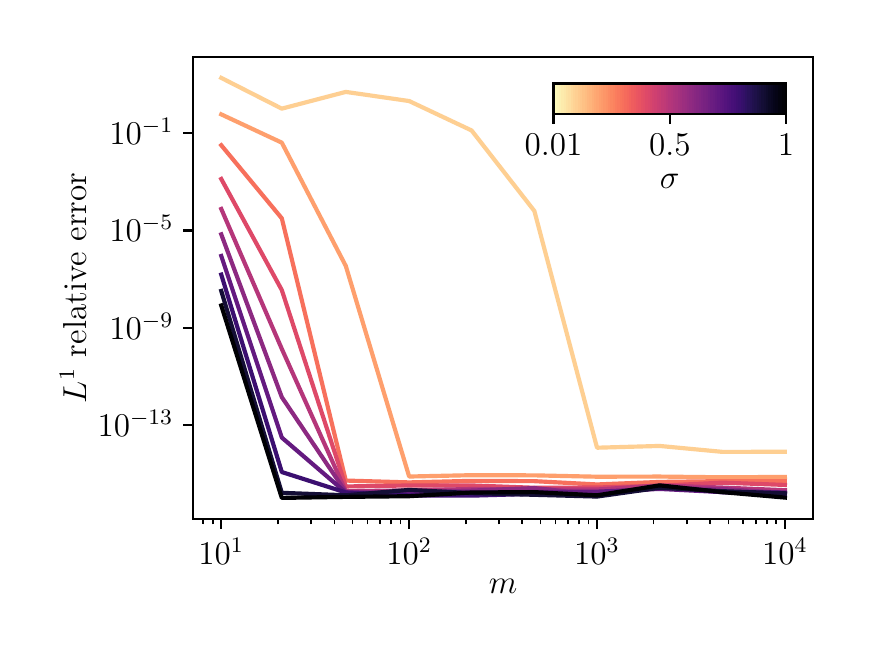
\begin{tikzpicture}
    \node at (0, 0) {%% Creator: Matplotlib, PGF backend
%%
%% To include the figure in your LaTeX document, write
%%   \input{<filename>.pgf}
%%
%% Make sure the required packages are loaded in your preamble
%%   \usepackage{pgf}
%%
%% Also ensure that all the required font packages are loaded; for instance,
%% the lmodern package is sometimes necessary when using math font.
%%   \usepackage{lmodern}
%%
%% Figures using additional raster images can only be included by \input if
%% they are in the same directory as the main LaTeX file. For loading figures
%% from other directories you can use the `import` package
%%   \usepackage{import}
%%
%% and then include the figures with
%%   \import{<path to file>}{<filename>.pgf}
%%
%% Matplotlib used the following preamble
%%   \def\mathdefault#1{#1}
%%   \everymath=\expandafter{\the\everymath\displaystyle}
%%   \IfFileExists{scrextend.sty}{
%%     \usepackage[fontsize=12.000000pt]{scrextend}
%%   }{
%%     \renewcommand{\normalsize}{\fontsize{12.000000}{14.400000}\selectfont}
%%     \normalsize
%%   }
%%   
%%   \ifdefined\pdftexversion\else  % non-pdftex case.
%%     \usepackage{fontspec}
%%     \setmainfont{DejaVuSans.ttf}[Path=\detokenize{/opt/hostedtoolcache/Python/3.12.9/x64/lib/python3.12/site-packages/matplotlib/mpl-data/fonts/ttf/}]
%%     \setsansfont{DejaVuSans.ttf}[Path=\detokenize{/opt/hostedtoolcache/Python/3.12.9/x64/lib/python3.12/site-packages/matplotlib/mpl-data/fonts/ttf/}]
%%     \setmonofont{DejaVuSansMono.ttf}[Path=\detokenize{/opt/hostedtoolcache/Python/3.12.9/x64/lib/python3.12/site-packages/matplotlib/mpl-data/fonts/ttf/}]
%%   \fi
%%   \makeatletter\@ifpackageloaded{underscore}{}{\usepackage[strings]{underscore}}\makeatother
%%
\begingroup%
\makeatletter%
\begin{pgfpicture}%
\pgfpathrectangle{\pgfpointorigin}{\pgfqpoint{3.980942in}{2.959073in}}%
\pgfusepath{use as bounding box, clip}%
\begin{pgfscope}%
\pgfsetbuttcap%
\pgfsetmiterjoin%
\definecolor{currentfill}{rgb}{1.000000,1.000000,1.000000}%
\pgfsetfillcolor{currentfill}%
\pgfsetlinewidth{0.000000pt}%
\definecolor{currentstroke}{rgb}{1.000000,1.000000,1.000000}%
\pgfsetstrokecolor{currentstroke}%
\pgfsetdash{}{0pt}%
\pgfpathmoveto{\pgfqpoint{0.000000in}{-0.000000in}}%
\pgfpathlineto{\pgfqpoint{3.980942in}{-0.000000in}}%
\pgfpathlineto{\pgfqpoint{3.980942in}{2.959073in}}%
\pgfpathlineto{\pgfqpoint{0.000000in}{2.959073in}}%
\pgfpathlineto{\pgfqpoint{0.000000in}{-0.000000in}}%
\pgfpathclose%
\pgfusepath{fill}%
\end{pgfscope}%
\begin{pgfscope}%
\pgfsetbuttcap%
\pgfsetmiterjoin%
\definecolor{currentfill}{rgb}{1.000000,1.000000,1.000000}%
\pgfsetfillcolor{currentfill}%
\pgfsetlinewidth{0.000000pt}%
\definecolor{currentstroke}{rgb}{0.000000,0.000000,0.000000}%
\pgfsetstrokecolor{currentstroke}%
\pgfsetstrokeopacity{0.000000}%
\pgfsetdash{}{0pt}%
\pgfpathmoveto{\pgfqpoint{0.780942in}{0.549073in}}%
\pgfpathlineto{\pgfqpoint{3.880942in}{0.549073in}}%
\pgfpathlineto{\pgfqpoint{3.880942in}{2.859073in}}%
\pgfpathlineto{\pgfqpoint{0.780942in}{2.859073in}}%
\pgfpathlineto{\pgfqpoint{0.780942in}{0.549073in}}%
\pgfpathclose%
\pgfusepath{fill}%
\end{pgfscope}%
\begin{pgfscope}%
\pgfsetbuttcap%
\pgfsetroundjoin%
\definecolor{currentfill}{rgb}{0.000000,0.000000,0.000000}%
\pgfsetfillcolor{currentfill}%
\pgfsetlinewidth{0.803000pt}%
\definecolor{currentstroke}{rgb}{0.000000,0.000000,0.000000}%
\pgfsetstrokecolor{currentstroke}%
\pgfsetdash{}{0pt}%
\pgfsys@defobject{currentmarker}{\pgfqpoint{0.000000in}{-0.048611in}}{\pgfqpoint{0.000000in}{0.000000in}}{%
\pgfpathmoveto{\pgfqpoint{0.000000in}{0.000000in}}%
\pgfpathlineto{\pgfqpoint{0.000000in}{-0.048611in}}%
\pgfusepath{stroke,fill}%
}%
\begin{pgfscope}%
\pgfsys@transformshift{0.921851in}{0.549073in}%
\pgfsys@useobject{currentmarker}{}%
\end{pgfscope}%
\end{pgfscope}%
\begin{pgfscope}%
\definecolor{textcolor}{rgb}{0.000000,0.000000,0.000000}%
\pgfsetstrokecolor{textcolor}%
\pgfsetfillcolor{textcolor}%
\pgftext[x=0.921851in,y=0.451851in,,top]{\color{textcolor}{\rmfamily\fontsize{12.000000}{14.400000}\selectfont\catcode`\^=\active\def^{\ifmmode\sp\else\^{}\fi}\catcode`\%=\active\def%{\%}$\mathdefault{10^{1}}$}}%
\end{pgfscope}%
\begin{pgfscope}%
\pgfsetbuttcap%
\pgfsetroundjoin%
\definecolor{currentfill}{rgb}{0.000000,0.000000,0.000000}%
\pgfsetfillcolor{currentfill}%
\pgfsetlinewidth{0.803000pt}%
\definecolor{currentstroke}{rgb}{0.000000,0.000000,0.000000}%
\pgfsetstrokecolor{currentstroke}%
\pgfsetdash{}{0pt}%
\pgfsys@defobject{currentmarker}{\pgfqpoint{0.000000in}{-0.048611in}}{\pgfqpoint{0.000000in}{0.000000in}}{%
\pgfpathmoveto{\pgfqpoint{0.000000in}{0.000000in}}%
\pgfpathlineto{\pgfqpoint{0.000000in}{-0.048611in}}%
\pgfusepath{stroke,fill}%
}%
\begin{pgfscope}%
\pgfsys@transformshift{1.861245in}{0.549073in}%
\pgfsys@useobject{currentmarker}{}%
\end{pgfscope}%
\end{pgfscope}%
\begin{pgfscope}%
\definecolor{textcolor}{rgb}{0.000000,0.000000,0.000000}%
\pgfsetstrokecolor{textcolor}%
\pgfsetfillcolor{textcolor}%
\pgftext[x=1.861245in,y=0.451851in,,top]{\color{textcolor}{\rmfamily\fontsize{12.000000}{14.400000}\selectfont\catcode`\^=\active\def^{\ifmmode\sp\else\^{}\fi}\catcode`\%=\active\def%{\%}$\mathdefault{10^{2}}$}}%
\end{pgfscope}%
\begin{pgfscope}%
\pgfsetbuttcap%
\pgfsetroundjoin%
\definecolor{currentfill}{rgb}{0.000000,0.000000,0.000000}%
\pgfsetfillcolor{currentfill}%
\pgfsetlinewidth{0.803000pt}%
\definecolor{currentstroke}{rgb}{0.000000,0.000000,0.000000}%
\pgfsetstrokecolor{currentstroke}%
\pgfsetdash{}{0pt}%
\pgfsys@defobject{currentmarker}{\pgfqpoint{0.000000in}{-0.048611in}}{\pgfqpoint{0.000000in}{0.000000in}}{%
\pgfpathmoveto{\pgfqpoint{0.000000in}{0.000000in}}%
\pgfpathlineto{\pgfqpoint{0.000000in}{-0.048611in}}%
\pgfusepath{stroke,fill}%
}%
\begin{pgfscope}%
\pgfsys@transformshift{2.800639in}{0.549073in}%
\pgfsys@useobject{currentmarker}{}%
\end{pgfscope}%
\end{pgfscope}%
\begin{pgfscope}%
\definecolor{textcolor}{rgb}{0.000000,0.000000,0.000000}%
\pgfsetstrokecolor{textcolor}%
\pgfsetfillcolor{textcolor}%
\pgftext[x=2.800639in,y=0.451851in,,top]{\color{textcolor}{\rmfamily\fontsize{12.000000}{14.400000}\selectfont\catcode`\^=\active\def^{\ifmmode\sp\else\^{}\fi}\catcode`\%=\active\def%{\%}$\mathdefault{10^{3}}$}}%
\end{pgfscope}%
\begin{pgfscope}%
\pgfsetbuttcap%
\pgfsetroundjoin%
\definecolor{currentfill}{rgb}{0.000000,0.000000,0.000000}%
\pgfsetfillcolor{currentfill}%
\pgfsetlinewidth{0.803000pt}%
\definecolor{currentstroke}{rgb}{0.000000,0.000000,0.000000}%
\pgfsetstrokecolor{currentstroke}%
\pgfsetdash{}{0pt}%
\pgfsys@defobject{currentmarker}{\pgfqpoint{0.000000in}{-0.048611in}}{\pgfqpoint{0.000000in}{0.000000in}}{%
\pgfpathmoveto{\pgfqpoint{0.000000in}{0.000000in}}%
\pgfpathlineto{\pgfqpoint{0.000000in}{-0.048611in}}%
\pgfusepath{stroke,fill}%
}%
\begin{pgfscope}%
\pgfsys@transformshift{3.740033in}{0.549073in}%
\pgfsys@useobject{currentmarker}{}%
\end{pgfscope}%
\end{pgfscope}%
\begin{pgfscope}%
\definecolor{textcolor}{rgb}{0.000000,0.000000,0.000000}%
\pgfsetstrokecolor{textcolor}%
\pgfsetfillcolor{textcolor}%
\pgftext[x=3.740033in,y=0.451851in,,top]{\color{textcolor}{\rmfamily\fontsize{12.000000}{14.400000}\selectfont\catcode`\^=\active\def^{\ifmmode\sp\else\^{}\fi}\catcode`\%=\active\def%{\%}$\mathdefault{10^{4}}$}}%
\end{pgfscope}%
\begin{pgfscope}%
\pgfsetbuttcap%
\pgfsetroundjoin%
\definecolor{currentfill}{rgb}{0.000000,0.000000,0.000000}%
\pgfsetfillcolor{currentfill}%
\pgfsetlinewidth{0.602250pt}%
\definecolor{currentstroke}{rgb}{0.000000,0.000000,0.000000}%
\pgfsetstrokecolor{currentstroke}%
\pgfsetdash{}{0pt}%
\pgfsys@defobject{currentmarker}{\pgfqpoint{0.000000in}{-0.027778in}}{\pgfqpoint{0.000000in}{0.000000in}}{%
\pgfpathmoveto{\pgfqpoint{0.000000in}{0.000000in}}%
\pgfpathlineto{\pgfqpoint{0.000000in}{-0.027778in}}%
\pgfusepath{stroke,fill}%
}%
\begin{pgfscope}%
\pgfsys@transformshift{0.830814in}{0.549073in}%
\pgfsys@useobject{currentmarker}{}%
\end{pgfscope}%
\end{pgfscope}%
\begin{pgfscope}%
\pgfsetbuttcap%
\pgfsetroundjoin%
\definecolor{currentfill}{rgb}{0.000000,0.000000,0.000000}%
\pgfsetfillcolor{currentfill}%
\pgfsetlinewidth{0.602250pt}%
\definecolor{currentstroke}{rgb}{0.000000,0.000000,0.000000}%
\pgfsetstrokecolor{currentstroke}%
\pgfsetdash{}{0pt}%
\pgfsys@defobject{currentmarker}{\pgfqpoint{0.000000in}{-0.027778in}}{\pgfqpoint{0.000000in}{0.000000in}}{%
\pgfpathmoveto{\pgfqpoint{0.000000in}{0.000000in}}%
\pgfpathlineto{\pgfqpoint{0.000000in}{-0.027778in}}%
\pgfusepath{stroke,fill}%
}%
\begin{pgfscope}%
\pgfsys@transformshift{0.878867in}{0.549073in}%
\pgfsys@useobject{currentmarker}{}%
\end{pgfscope}%
\end{pgfscope}%
\begin{pgfscope}%
\pgfsetbuttcap%
\pgfsetroundjoin%
\definecolor{currentfill}{rgb}{0.000000,0.000000,0.000000}%
\pgfsetfillcolor{currentfill}%
\pgfsetlinewidth{0.602250pt}%
\definecolor{currentstroke}{rgb}{0.000000,0.000000,0.000000}%
\pgfsetstrokecolor{currentstroke}%
\pgfsetdash{}{0pt}%
\pgfsys@defobject{currentmarker}{\pgfqpoint{0.000000in}{-0.027778in}}{\pgfqpoint{0.000000in}{0.000000in}}{%
\pgfpathmoveto{\pgfqpoint{0.000000in}{0.000000in}}%
\pgfpathlineto{\pgfqpoint{0.000000in}{-0.027778in}}%
\pgfusepath{stroke,fill}%
}%
\begin{pgfscope}%
\pgfsys@transformshift{1.204637in}{0.549073in}%
\pgfsys@useobject{currentmarker}{}%
\end{pgfscope}%
\end{pgfscope}%
\begin{pgfscope}%
\pgfsetbuttcap%
\pgfsetroundjoin%
\definecolor{currentfill}{rgb}{0.000000,0.000000,0.000000}%
\pgfsetfillcolor{currentfill}%
\pgfsetlinewidth{0.602250pt}%
\definecolor{currentstroke}{rgb}{0.000000,0.000000,0.000000}%
\pgfsetstrokecolor{currentstroke}%
\pgfsetdash{}{0pt}%
\pgfsys@defobject{currentmarker}{\pgfqpoint{0.000000in}{-0.027778in}}{\pgfqpoint{0.000000in}{0.000000in}}{%
\pgfpathmoveto{\pgfqpoint{0.000000in}{0.000000in}}%
\pgfpathlineto{\pgfqpoint{0.000000in}{-0.027778in}}%
\pgfusepath{stroke,fill}%
}%
\begin{pgfscope}%
\pgfsys@transformshift{1.370056in}{0.549073in}%
\pgfsys@useobject{currentmarker}{}%
\end{pgfscope}%
\end{pgfscope}%
\begin{pgfscope}%
\pgfsetbuttcap%
\pgfsetroundjoin%
\definecolor{currentfill}{rgb}{0.000000,0.000000,0.000000}%
\pgfsetfillcolor{currentfill}%
\pgfsetlinewidth{0.602250pt}%
\definecolor{currentstroke}{rgb}{0.000000,0.000000,0.000000}%
\pgfsetstrokecolor{currentstroke}%
\pgfsetdash{}{0pt}%
\pgfsys@defobject{currentmarker}{\pgfqpoint{0.000000in}{-0.027778in}}{\pgfqpoint{0.000000in}{0.000000in}}{%
\pgfpathmoveto{\pgfqpoint{0.000000in}{0.000000in}}%
\pgfpathlineto{\pgfqpoint{0.000000in}{-0.027778in}}%
\pgfusepath{stroke,fill}%
}%
\begin{pgfscope}%
\pgfsys@transformshift{1.487423in}{0.549073in}%
\pgfsys@useobject{currentmarker}{}%
\end{pgfscope}%
\end{pgfscope}%
\begin{pgfscope}%
\pgfsetbuttcap%
\pgfsetroundjoin%
\definecolor{currentfill}{rgb}{0.000000,0.000000,0.000000}%
\pgfsetfillcolor{currentfill}%
\pgfsetlinewidth{0.602250pt}%
\definecolor{currentstroke}{rgb}{0.000000,0.000000,0.000000}%
\pgfsetstrokecolor{currentstroke}%
\pgfsetdash{}{0pt}%
\pgfsys@defobject{currentmarker}{\pgfqpoint{0.000000in}{-0.027778in}}{\pgfqpoint{0.000000in}{0.000000in}}{%
\pgfpathmoveto{\pgfqpoint{0.000000in}{0.000000in}}%
\pgfpathlineto{\pgfqpoint{0.000000in}{-0.027778in}}%
\pgfusepath{stroke,fill}%
}%
\begin{pgfscope}%
\pgfsys@transformshift{1.578459in}{0.549073in}%
\pgfsys@useobject{currentmarker}{}%
\end{pgfscope}%
\end{pgfscope}%
\begin{pgfscope}%
\pgfsetbuttcap%
\pgfsetroundjoin%
\definecolor{currentfill}{rgb}{0.000000,0.000000,0.000000}%
\pgfsetfillcolor{currentfill}%
\pgfsetlinewidth{0.602250pt}%
\definecolor{currentstroke}{rgb}{0.000000,0.000000,0.000000}%
\pgfsetstrokecolor{currentstroke}%
\pgfsetdash{}{0pt}%
\pgfsys@defobject{currentmarker}{\pgfqpoint{0.000000in}{-0.027778in}}{\pgfqpoint{0.000000in}{0.000000in}}{%
\pgfpathmoveto{\pgfqpoint{0.000000in}{0.000000in}}%
\pgfpathlineto{\pgfqpoint{0.000000in}{-0.027778in}}%
\pgfusepath{stroke,fill}%
}%
\begin{pgfscope}%
\pgfsys@transformshift{1.652842in}{0.549073in}%
\pgfsys@useobject{currentmarker}{}%
\end{pgfscope}%
\end{pgfscope}%
\begin{pgfscope}%
\pgfsetbuttcap%
\pgfsetroundjoin%
\definecolor{currentfill}{rgb}{0.000000,0.000000,0.000000}%
\pgfsetfillcolor{currentfill}%
\pgfsetlinewidth{0.602250pt}%
\definecolor{currentstroke}{rgb}{0.000000,0.000000,0.000000}%
\pgfsetstrokecolor{currentstroke}%
\pgfsetdash{}{0pt}%
\pgfsys@defobject{currentmarker}{\pgfqpoint{0.000000in}{-0.027778in}}{\pgfqpoint{0.000000in}{0.000000in}}{%
\pgfpathmoveto{\pgfqpoint{0.000000in}{0.000000in}}%
\pgfpathlineto{\pgfqpoint{0.000000in}{-0.027778in}}%
\pgfusepath{stroke,fill}%
}%
\begin{pgfscope}%
\pgfsys@transformshift{1.715731in}{0.549073in}%
\pgfsys@useobject{currentmarker}{}%
\end{pgfscope}%
\end{pgfscope}%
\begin{pgfscope}%
\pgfsetbuttcap%
\pgfsetroundjoin%
\definecolor{currentfill}{rgb}{0.000000,0.000000,0.000000}%
\pgfsetfillcolor{currentfill}%
\pgfsetlinewidth{0.602250pt}%
\definecolor{currentstroke}{rgb}{0.000000,0.000000,0.000000}%
\pgfsetstrokecolor{currentstroke}%
\pgfsetdash{}{0pt}%
\pgfsys@defobject{currentmarker}{\pgfqpoint{0.000000in}{-0.027778in}}{\pgfqpoint{0.000000in}{0.000000in}}{%
\pgfpathmoveto{\pgfqpoint{0.000000in}{0.000000in}}%
\pgfpathlineto{\pgfqpoint{0.000000in}{-0.027778in}}%
\pgfusepath{stroke,fill}%
}%
\begin{pgfscope}%
\pgfsys@transformshift{1.770208in}{0.549073in}%
\pgfsys@useobject{currentmarker}{}%
\end{pgfscope}%
\end{pgfscope}%
\begin{pgfscope}%
\pgfsetbuttcap%
\pgfsetroundjoin%
\definecolor{currentfill}{rgb}{0.000000,0.000000,0.000000}%
\pgfsetfillcolor{currentfill}%
\pgfsetlinewidth{0.602250pt}%
\definecolor{currentstroke}{rgb}{0.000000,0.000000,0.000000}%
\pgfsetstrokecolor{currentstroke}%
\pgfsetdash{}{0pt}%
\pgfsys@defobject{currentmarker}{\pgfqpoint{0.000000in}{-0.027778in}}{\pgfqpoint{0.000000in}{0.000000in}}{%
\pgfpathmoveto{\pgfqpoint{0.000000in}{0.000000in}}%
\pgfpathlineto{\pgfqpoint{0.000000in}{-0.027778in}}%
\pgfusepath{stroke,fill}%
}%
\begin{pgfscope}%
\pgfsys@transformshift{1.818261in}{0.549073in}%
\pgfsys@useobject{currentmarker}{}%
\end{pgfscope}%
\end{pgfscope}%
\begin{pgfscope}%
\pgfsetbuttcap%
\pgfsetroundjoin%
\definecolor{currentfill}{rgb}{0.000000,0.000000,0.000000}%
\pgfsetfillcolor{currentfill}%
\pgfsetlinewidth{0.602250pt}%
\definecolor{currentstroke}{rgb}{0.000000,0.000000,0.000000}%
\pgfsetstrokecolor{currentstroke}%
\pgfsetdash{}{0pt}%
\pgfsys@defobject{currentmarker}{\pgfqpoint{0.000000in}{-0.027778in}}{\pgfqpoint{0.000000in}{0.000000in}}{%
\pgfpathmoveto{\pgfqpoint{0.000000in}{0.000000in}}%
\pgfpathlineto{\pgfqpoint{0.000000in}{-0.027778in}}%
\pgfusepath{stroke,fill}%
}%
\begin{pgfscope}%
\pgfsys@transformshift{2.144031in}{0.549073in}%
\pgfsys@useobject{currentmarker}{}%
\end{pgfscope}%
\end{pgfscope}%
\begin{pgfscope}%
\pgfsetbuttcap%
\pgfsetroundjoin%
\definecolor{currentfill}{rgb}{0.000000,0.000000,0.000000}%
\pgfsetfillcolor{currentfill}%
\pgfsetlinewidth{0.602250pt}%
\definecolor{currentstroke}{rgb}{0.000000,0.000000,0.000000}%
\pgfsetstrokecolor{currentstroke}%
\pgfsetdash{}{0pt}%
\pgfsys@defobject{currentmarker}{\pgfqpoint{0.000000in}{-0.027778in}}{\pgfqpoint{0.000000in}{0.000000in}}{%
\pgfpathmoveto{\pgfqpoint{0.000000in}{0.000000in}}%
\pgfpathlineto{\pgfqpoint{0.000000in}{-0.027778in}}%
\pgfusepath{stroke,fill}%
}%
\begin{pgfscope}%
\pgfsys@transformshift{2.309450in}{0.549073in}%
\pgfsys@useobject{currentmarker}{}%
\end{pgfscope}%
\end{pgfscope}%
\begin{pgfscope}%
\pgfsetbuttcap%
\pgfsetroundjoin%
\definecolor{currentfill}{rgb}{0.000000,0.000000,0.000000}%
\pgfsetfillcolor{currentfill}%
\pgfsetlinewidth{0.602250pt}%
\definecolor{currentstroke}{rgb}{0.000000,0.000000,0.000000}%
\pgfsetstrokecolor{currentstroke}%
\pgfsetdash{}{0pt}%
\pgfsys@defobject{currentmarker}{\pgfqpoint{0.000000in}{-0.027778in}}{\pgfqpoint{0.000000in}{0.000000in}}{%
\pgfpathmoveto{\pgfqpoint{0.000000in}{0.000000in}}%
\pgfpathlineto{\pgfqpoint{0.000000in}{-0.027778in}}%
\pgfusepath{stroke,fill}%
}%
\begin{pgfscope}%
\pgfsys@transformshift{2.426816in}{0.549073in}%
\pgfsys@useobject{currentmarker}{}%
\end{pgfscope}%
\end{pgfscope}%
\begin{pgfscope}%
\pgfsetbuttcap%
\pgfsetroundjoin%
\definecolor{currentfill}{rgb}{0.000000,0.000000,0.000000}%
\pgfsetfillcolor{currentfill}%
\pgfsetlinewidth{0.602250pt}%
\definecolor{currentstroke}{rgb}{0.000000,0.000000,0.000000}%
\pgfsetstrokecolor{currentstroke}%
\pgfsetdash{}{0pt}%
\pgfsys@defobject{currentmarker}{\pgfqpoint{0.000000in}{-0.027778in}}{\pgfqpoint{0.000000in}{0.000000in}}{%
\pgfpathmoveto{\pgfqpoint{0.000000in}{0.000000in}}%
\pgfpathlineto{\pgfqpoint{0.000000in}{-0.027778in}}%
\pgfusepath{stroke,fill}%
}%
\begin{pgfscope}%
\pgfsys@transformshift{2.517853in}{0.549073in}%
\pgfsys@useobject{currentmarker}{}%
\end{pgfscope}%
\end{pgfscope}%
\begin{pgfscope}%
\pgfsetbuttcap%
\pgfsetroundjoin%
\definecolor{currentfill}{rgb}{0.000000,0.000000,0.000000}%
\pgfsetfillcolor{currentfill}%
\pgfsetlinewidth{0.602250pt}%
\definecolor{currentstroke}{rgb}{0.000000,0.000000,0.000000}%
\pgfsetstrokecolor{currentstroke}%
\pgfsetdash{}{0pt}%
\pgfsys@defobject{currentmarker}{\pgfqpoint{0.000000in}{-0.027778in}}{\pgfqpoint{0.000000in}{0.000000in}}{%
\pgfpathmoveto{\pgfqpoint{0.000000in}{0.000000in}}%
\pgfpathlineto{\pgfqpoint{0.000000in}{-0.027778in}}%
\pgfusepath{stroke,fill}%
}%
\begin{pgfscope}%
\pgfsys@transformshift{2.592236in}{0.549073in}%
\pgfsys@useobject{currentmarker}{}%
\end{pgfscope}%
\end{pgfscope}%
\begin{pgfscope}%
\pgfsetbuttcap%
\pgfsetroundjoin%
\definecolor{currentfill}{rgb}{0.000000,0.000000,0.000000}%
\pgfsetfillcolor{currentfill}%
\pgfsetlinewidth{0.602250pt}%
\definecolor{currentstroke}{rgb}{0.000000,0.000000,0.000000}%
\pgfsetstrokecolor{currentstroke}%
\pgfsetdash{}{0pt}%
\pgfsys@defobject{currentmarker}{\pgfqpoint{0.000000in}{-0.027778in}}{\pgfqpoint{0.000000in}{0.000000in}}{%
\pgfpathmoveto{\pgfqpoint{0.000000in}{0.000000in}}%
\pgfpathlineto{\pgfqpoint{0.000000in}{-0.027778in}}%
\pgfusepath{stroke,fill}%
}%
\begin{pgfscope}%
\pgfsys@transformshift{2.655125in}{0.549073in}%
\pgfsys@useobject{currentmarker}{}%
\end{pgfscope}%
\end{pgfscope}%
\begin{pgfscope}%
\pgfsetbuttcap%
\pgfsetroundjoin%
\definecolor{currentfill}{rgb}{0.000000,0.000000,0.000000}%
\pgfsetfillcolor{currentfill}%
\pgfsetlinewidth{0.602250pt}%
\definecolor{currentstroke}{rgb}{0.000000,0.000000,0.000000}%
\pgfsetstrokecolor{currentstroke}%
\pgfsetdash{}{0pt}%
\pgfsys@defobject{currentmarker}{\pgfqpoint{0.000000in}{-0.027778in}}{\pgfqpoint{0.000000in}{0.000000in}}{%
\pgfpathmoveto{\pgfqpoint{0.000000in}{0.000000in}}%
\pgfpathlineto{\pgfqpoint{0.000000in}{-0.027778in}}%
\pgfusepath{stroke,fill}%
}%
\begin{pgfscope}%
\pgfsys@transformshift{2.709602in}{0.549073in}%
\pgfsys@useobject{currentmarker}{}%
\end{pgfscope}%
\end{pgfscope}%
\begin{pgfscope}%
\pgfsetbuttcap%
\pgfsetroundjoin%
\definecolor{currentfill}{rgb}{0.000000,0.000000,0.000000}%
\pgfsetfillcolor{currentfill}%
\pgfsetlinewidth{0.602250pt}%
\definecolor{currentstroke}{rgb}{0.000000,0.000000,0.000000}%
\pgfsetstrokecolor{currentstroke}%
\pgfsetdash{}{0pt}%
\pgfsys@defobject{currentmarker}{\pgfqpoint{0.000000in}{-0.027778in}}{\pgfqpoint{0.000000in}{0.000000in}}{%
\pgfpathmoveto{\pgfqpoint{0.000000in}{0.000000in}}%
\pgfpathlineto{\pgfqpoint{0.000000in}{-0.027778in}}%
\pgfusepath{stroke,fill}%
}%
\begin{pgfscope}%
\pgfsys@transformshift{2.757655in}{0.549073in}%
\pgfsys@useobject{currentmarker}{}%
\end{pgfscope}%
\end{pgfscope}%
\begin{pgfscope}%
\pgfsetbuttcap%
\pgfsetroundjoin%
\definecolor{currentfill}{rgb}{0.000000,0.000000,0.000000}%
\pgfsetfillcolor{currentfill}%
\pgfsetlinewidth{0.602250pt}%
\definecolor{currentstroke}{rgb}{0.000000,0.000000,0.000000}%
\pgfsetstrokecolor{currentstroke}%
\pgfsetdash{}{0pt}%
\pgfsys@defobject{currentmarker}{\pgfqpoint{0.000000in}{-0.027778in}}{\pgfqpoint{0.000000in}{0.000000in}}{%
\pgfpathmoveto{\pgfqpoint{0.000000in}{0.000000in}}%
\pgfpathlineto{\pgfqpoint{0.000000in}{-0.027778in}}%
\pgfusepath{stroke,fill}%
}%
\begin{pgfscope}%
\pgfsys@transformshift{3.083425in}{0.549073in}%
\pgfsys@useobject{currentmarker}{}%
\end{pgfscope}%
\end{pgfscope}%
\begin{pgfscope}%
\pgfsetbuttcap%
\pgfsetroundjoin%
\definecolor{currentfill}{rgb}{0.000000,0.000000,0.000000}%
\pgfsetfillcolor{currentfill}%
\pgfsetlinewidth{0.602250pt}%
\definecolor{currentstroke}{rgb}{0.000000,0.000000,0.000000}%
\pgfsetstrokecolor{currentstroke}%
\pgfsetdash{}{0pt}%
\pgfsys@defobject{currentmarker}{\pgfqpoint{0.000000in}{-0.027778in}}{\pgfqpoint{0.000000in}{0.000000in}}{%
\pgfpathmoveto{\pgfqpoint{0.000000in}{0.000000in}}%
\pgfpathlineto{\pgfqpoint{0.000000in}{-0.027778in}}%
\pgfusepath{stroke,fill}%
}%
\begin{pgfscope}%
\pgfsys@transformshift{3.248844in}{0.549073in}%
\pgfsys@useobject{currentmarker}{}%
\end{pgfscope}%
\end{pgfscope}%
\begin{pgfscope}%
\pgfsetbuttcap%
\pgfsetroundjoin%
\definecolor{currentfill}{rgb}{0.000000,0.000000,0.000000}%
\pgfsetfillcolor{currentfill}%
\pgfsetlinewidth{0.602250pt}%
\definecolor{currentstroke}{rgb}{0.000000,0.000000,0.000000}%
\pgfsetstrokecolor{currentstroke}%
\pgfsetdash{}{0pt}%
\pgfsys@defobject{currentmarker}{\pgfqpoint{0.000000in}{-0.027778in}}{\pgfqpoint{0.000000in}{0.000000in}}{%
\pgfpathmoveto{\pgfqpoint{0.000000in}{0.000000in}}%
\pgfpathlineto{\pgfqpoint{0.000000in}{-0.027778in}}%
\pgfusepath{stroke,fill}%
}%
\begin{pgfscope}%
\pgfsys@transformshift{3.366210in}{0.549073in}%
\pgfsys@useobject{currentmarker}{}%
\end{pgfscope}%
\end{pgfscope}%
\begin{pgfscope}%
\pgfsetbuttcap%
\pgfsetroundjoin%
\definecolor{currentfill}{rgb}{0.000000,0.000000,0.000000}%
\pgfsetfillcolor{currentfill}%
\pgfsetlinewidth{0.602250pt}%
\definecolor{currentstroke}{rgb}{0.000000,0.000000,0.000000}%
\pgfsetstrokecolor{currentstroke}%
\pgfsetdash{}{0pt}%
\pgfsys@defobject{currentmarker}{\pgfqpoint{0.000000in}{-0.027778in}}{\pgfqpoint{0.000000in}{0.000000in}}{%
\pgfpathmoveto{\pgfqpoint{0.000000in}{0.000000in}}%
\pgfpathlineto{\pgfqpoint{0.000000in}{-0.027778in}}%
\pgfusepath{stroke,fill}%
}%
\begin{pgfscope}%
\pgfsys@transformshift{3.457247in}{0.549073in}%
\pgfsys@useobject{currentmarker}{}%
\end{pgfscope}%
\end{pgfscope}%
\begin{pgfscope}%
\pgfsetbuttcap%
\pgfsetroundjoin%
\definecolor{currentfill}{rgb}{0.000000,0.000000,0.000000}%
\pgfsetfillcolor{currentfill}%
\pgfsetlinewidth{0.602250pt}%
\definecolor{currentstroke}{rgb}{0.000000,0.000000,0.000000}%
\pgfsetstrokecolor{currentstroke}%
\pgfsetdash{}{0pt}%
\pgfsys@defobject{currentmarker}{\pgfqpoint{0.000000in}{-0.027778in}}{\pgfqpoint{0.000000in}{0.000000in}}{%
\pgfpathmoveto{\pgfqpoint{0.000000in}{0.000000in}}%
\pgfpathlineto{\pgfqpoint{0.000000in}{-0.027778in}}%
\pgfusepath{stroke,fill}%
}%
\begin{pgfscope}%
\pgfsys@transformshift{3.531629in}{0.549073in}%
\pgfsys@useobject{currentmarker}{}%
\end{pgfscope}%
\end{pgfscope}%
\begin{pgfscope}%
\pgfsetbuttcap%
\pgfsetroundjoin%
\definecolor{currentfill}{rgb}{0.000000,0.000000,0.000000}%
\pgfsetfillcolor{currentfill}%
\pgfsetlinewidth{0.602250pt}%
\definecolor{currentstroke}{rgb}{0.000000,0.000000,0.000000}%
\pgfsetstrokecolor{currentstroke}%
\pgfsetdash{}{0pt}%
\pgfsys@defobject{currentmarker}{\pgfqpoint{0.000000in}{-0.027778in}}{\pgfqpoint{0.000000in}{0.000000in}}{%
\pgfpathmoveto{\pgfqpoint{0.000000in}{0.000000in}}%
\pgfpathlineto{\pgfqpoint{0.000000in}{-0.027778in}}%
\pgfusepath{stroke,fill}%
}%
\begin{pgfscope}%
\pgfsys@transformshift{3.594519in}{0.549073in}%
\pgfsys@useobject{currentmarker}{}%
\end{pgfscope}%
\end{pgfscope}%
\begin{pgfscope}%
\pgfsetbuttcap%
\pgfsetroundjoin%
\definecolor{currentfill}{rgb}{0.000000,0.000000,0.000000}%
\pgfsetfillcolor{currentfill}%
\pgfsetlinewidth{0.602250pt}%
\definecolor{currentstroke}{rgb}{0.000000,0.000000,0.000000}%
\pgfsetstrokecolor{currentstroke}%
\pgfsetdash{}{0pt}%
\pgfsys@defobject{currentmarker}{\pgfqpoint{0.000000in}{-0.027778in}}{\pgfqpoint{0.000000in}{0.000000in}}{%
\pgfpathmoveto{\pgfqpoint{0.000000in}{0.000000in}}%
\pgfpathlineto{\pgfqpoint{0.000000in}{-0.027778in}}%
\pgfusepath{stroke,fill}%
}%
\begin{pgfscope}%
\pgfsys@transformshift{3.648996in}{0.549073in}%
\pgfsys@useobject{currentmarker}{}%
\end{pgfscope}%
\end{pgfscope}%
\begin{pgfscope}%
\pgfsetbuttcap%
\pgfsetroundjoin%
\definecolor{currentfill}{rgb}{0.000000,0.000000,0.000000}%
\pgfsetfillcolor{currentfill}%
\pgfsetlinewidth{0.602250pt}%
\definecolor{currentstroke}{rgb}{0.000000,0.000000,0.000000}%
\pgfsetstrokecolor{currentstroke}%
\pgfsetdash{}{0pt}%
\pgfsys@defobject{currentmarker}{\pgfqpoint{0.000000in}{-0.027778in}}{\pgfqpoint{0.000000in}{0.000000in}}{%
\pgfpathmoveto{\pgfqpoint{0.000000in}{0.000000in}}%
\pgfpathlineto{\pgfqpoint{0.000000in}{-0.027778in}}%
\pgfusepath{stroke,fill}%
}%
\begin{pgfscope}%
\pgfsys@transformshift{3.697049in}{0.549073in}%
\pgfsys@useobject{currentmarker}{}%
\end{pgfscope}%
\end{pgfscope}%
\begin{pgfscope}%
\definecolor{textcolor}{rgb}{0.000000,0.000000,0.000000}%
\pgfsetstrokecolor{textcolor}%
\pgfsetfillcolor{textcolor}%
\pgftext[x=2.330942in,y=0.248148in,,top]{\color{textcolor}{\rmfamily\fontsize{12.000000}{14.400000}\selectfont\catcode`\^=\active\def^{\ifmmode\sp\else\^{}\fi}\catcode`\%=\active\def%{\%}$m$}}%
\end{pgfscope}%
\begin{pgfscope}%
\pgfsetbuttcap%
\pgfsetroundjoin%
\definecolor{currentfill}{rgb}{0.000000,0.000000,0.000000}%
\pgfsetfillcolor{currentfill}%
\pgfsetlinewidth{0.803000pt}%
\definecolor{currentstroke}{rgb}{0.000000,0.000000,0.000000}%
\pgfsetstrokecolor{currentstroke}%
\pgfsetdash{}{0pt}%
\pgfsys@defobject{currentmarker}{\pgfqpoint{-0.048611in}{0.000000in}}{\pgfqpoint{-0.000000in}{0.000000in}}{%
\pgfpathmoveto{\pgfqpoint{-0.000000in}{0.000000in}}%
\pgfpathlineto{\pgfqpoint{-0.048611in}{0.000000in}}%
\pgfusepath{stroke,fill}%
}%
\begin{pgfscope}%
\pgfsys@transformshift{0.780942in}{1.017484in}%
\pgfsys@useobject{currentmarker}{}%
\end{pgfscope}%
\end{pgfscope}%
\begin{pgfscope}%
\definecolor{textcolor}{rgb}{0.000000,0.000000,0.000000}%
\pgfsetstrokecolor{textcolor}%
\pgfsetfillcolor{textcolor}%
\pgftext[x=0.303703in, y=0.959613in, left, base]{\color{textcolor}{\rmfamily\fontsize{12.000000}{14.400000}\selectfont\catcode`\^=\active\def^{\ifmmode\sp\else\^{}\fi}\catcode`\%=\active\def%{\%}$\mathdefault{10^{-13}}$}}%
\end{pgfscope}%
\begin{pgfscope}%
\pgfsetbuttcap%
\pgfsetroundjoin%
\definecolor{currentfill}{rgb}{0.000000,0.000000,0.000000}%
\pgfsetfillcolor{currentfill}%
\pgfsetlinewidth{0.803000pt}%
\definecolor{currentstroke}{rgb}{0.000000,0.000000,0.000000}%
\pgfsetstrokecolor{currentstroke}%
\pgfsetdash{}{0pt}%
\pgfsys@defobject{currentmarker}{\pgfqpoint{-0.048611in}{0.000000in}}{\pgfqpoint{-0.000000in}{0.000000in}}{%
\pgfpathmoveto{\pgfqpoint{-0.000000in}{0.000000in}}%
\pgfpathlineto{\pgfqpoint{-0.048611in}{0.000000in}}%
\pgfusepath{stroke,fill}%
}%
\begin{pgfscope}%
\pgfsys@transformshift{0.780942in}{1.504505in}%
\pgfsys@useobject{currentmarker}{}%
\end{pgfscope}%
\end{pgfscope}%
\begin{pgfscope}%
\definecolor{textcolor}{rgb}{0.000000,0.000000,0.000000}%
\pgfsetstrokecolor{textcolor}%
\pgfsetfillcolor{textcolor}%
\pgftext[x=0.362732in, y=1.446635in, left, base]{\color{textcolor}{\rmfamily\fontsize{12.000000}{14.400000}\selectfont\catcode`\^=\active\def^{\ifmmode\sp\else\^{}\fi}\catcode`\%=\active\def%{\%}$\mathdefault{10^{-9}}$}}%
\end{pgfscope}%
\begin{pgfscope}%
\pgfsetbuttcap%
\pgfsetroundjoin%
\definecolor{currentfill}{rgb}{0.000000,0.000000,0.000000}%
\pgfsetfillcolor{currentfill}%
\pgfsetlinewidth{0.803000pt}%
\definecolor{currentstroke}{rgb}{0.000000,0.000000,0.000000}%
\pgfsetstrokecolor{currentstroke}%
\pgfsetdash{}{0pt}%
\pgfsys@defobject{currentmarker}{\pgfqpoint{-0.048611in}{0.000000in}}{\pgfqpoint{-0.000000in}{0.000000in}}{%
\pgfpathmoveto{\pgfqpoint{-0.000000in}{0.000000in}}%
\pgfpathlineto{\pgfqpoint{-0.048611in}{0.000000in}}%
\pgfusepath{stroke,fill}%
}%
\begin{pgfscope}%
\pgfsys@transformshift{0.780942in}{1.991526in}%
\pgfsys@useobject{currentmarker}{}%
\end{pgfscope}%
\end{pgfscope}%
\begin{pgfscope}%
\definecolor{textcolor}{rgb}{0.000000,0.000000,0.000000}%
\pgfsetstrokecolor{textcolor}%
\pgfsetfillcolor{textcolor}%
\pgftext[x=0.362732in, y=1.933656in, left, base]{\color{textcolor}{\rmfamily\fontsize{12.000000}{14.400000}\selectfont\catcode`\^=\active\def^{\ifmmode\sp\else\^{}\fi}\catcode`\%=\active\def%{\%}$\mathdefault{10^{-5}}$}}%
\end{pgfscope}%
\begin{pgfscope}%
\pgfsetbuttcap%
\pgfsetroundjoin%
\definecolor{currentfill}{rgb}{0.000000,0.000000,0.000000}%
\pgfsetfillcolor{currentfill}%
\pgfsetlinewidth{0.803000pt}%
\definecolor{currentstroke}{rgb}{0.000000,0.000000,0.000000}%
\pgfsetstrokecolor{currentstroke}%
\pgfsetdash{}{0pt}%
\pgfsys@defobject{currentmarker}{\pgfqpoint{-0.048611in}{0.000000in}}{\pgfqpoint{-0.000000in}{0.000000in}}{%
\pgfpathmoveto{\pgfqpoint{-0.000000in}{0.000000in}}%
\pgfpathlineto{\pgfqpoint{-0.048611in}{0.000000in}}%
\pgfusepath{stroke,fill}%
}%
\begin{pgfscope}%
\pgfsys@transformshift{0.780942in}{2.478547in}%
\pgfsys@useobject{currentmarker}{}%
\end{pgfscope}%
\end{pgfscope}%
\begin{pgfscope}%
\definecolor{textcolor}{rgb}{0.000000,0.000000,0.000000}%
\pgfsetstrokecolor{textcolor}%
\pgfsetfillcolor{textcolor}%
\pgftext[x=0.362732in, y=2.420677in, left, base]{\color{textcolor}{\rmfamily\fontsize{12.000000}{14.400000}\selectfont\catcode`\^=\active\def^{\ifmmode\sp\else\^{}\fi}\catcode`\%=\active\def%{\%}$\mathdefault{10^{-1}}$}}%
\end{pgfscope}%
\begin{pgfscope}%
\definecolor{textcolor}{rgb}{0.000000,0.000000,0.000000}%
\pgfsetstrokecolor{textcolor}%
\pgfsetfillcolor{textcolor}%
\pgftext[x=0.248147in,y=1.704073in,,bottom,rotate=90.000000]{\color{textcolor}{\rmfamily\fontsize{12.000000}{14.400000}\selectfont\catcode`\^=\active\def^{\ifmmode\sp\else\^{}\fi}\catcode`\%=\active\def%{\%}$L^1$ relative error}}%
\end{pgfscope}%
\begin{pgfscope}%
\pgfpathrectangle{\pgfqpoint{0.780942in}{0.549073in}}{\pgfqpoint{3.100000in}{2.310000in}}%
\pgfusepath{clip}%
\pgfsetrectcap%
\pgfsetroundjoin%
\pgfsetlinewidth{1.505625pt}%
\definecolor{currentstroke}{rgb}{0.995680,0.812706,0.572645}%
\pgfsetstrokecolor{currentstroke}%
\pgfsetdash{}{0pt}%
\pgfpathmoveto{\pgfqpoint{0.921851in}{2.754073in}}%
\pgfpathlineto{\pgfqpoint{1.224542in}{2.600303in}}%
\pgfpathlineto{\pgfqpoint{1.544442in}{2.684040in}}%
\pgfpathlineto{\pgfqpoint{1.861245in}{2.638362in}}%
\pgfpathlineto{\pgfqpoint{2.173536in}{2.491177in}}%
\pgfpathlineto{\pgfqpoint{2.487368in}{2.088576in}}%
\pgfpathlineto{\pgfqpoint{2.800639in}{0.904985in}}%
\pgfpathlineto{\pgfqpoint{3.113688in}{0.913831in}}%
\pgfpathlineto{\pgfqpoint{3.426850in}{0.884295in}}%
\pgfpathlineto{\pgfqpoint{3.740033in}{0.884513in}}%
\pgfusepath{stroke}%
\end{pgfscope}%
\begin{pgfscope}%
\pgfpathrectangle{\pgfqpoint{0.780942in}{0.549073in}}{\pgfqpoint{3.100000in}{2.310000in}}%
\pgfusepath{clip}%
\pgfsetrectcap%
\pgfsetroundjoin%
\pgfsetlinewidth{1.505625pt}%
\definecolor{currentstroke}{rgb}{0.994738,0.624350,0.427397}%
\pgfsetstrokecolor{currentstroke}%
\pgfsetdash{}{0pt}%
\pgfpathmoveto{\pgfqpoint{0.921851in}{2.571671in}}%
\pgfpathlineto{\pgfqpoint{1.224542in}{2.430243in}}%
\pgfpathlineto{\pgfqpoint{1.544442in}{1.813870in}}%
\pgfpathlineto{\pgfqpoint{1.861245in}{0.760953in}}%
\pgfpathlineto{\pgfqpoint{2.173536in}{0.767666in}}%
\pgfpathlineto{\pgfqpoint{2.487368in}{0.766766in}}%
\pgfpathlineto{\pgfqpoint{2.800639in}{0.759988in}}%
\pgfpathlineto{\pgfqpoint{3.113688in}{0.760731in}}%
\pgfpathlineto{\pgfqpoint{3.426850in}{0.757182in}}%
\pgfpathlineto{\pgfqpoint{3.740033in}{0.758860in}}%
\pgfusepath{stroke}%
\end{pgfscope}%
\begin{pgfscope}%
\pgfpathrectangle{\pgfqpoint{0.780942in}{0.549073in}}{\pgfqpoint{3.100000in}{2.310000in}}%
\pgfusepath{clip}%
\pgfsetrectcap%
\pgfsetroundjoin%
\pgfsetlinewidth{1.505625pt}%
\definecolor{currentstroke}{rgb}{0.967671,0.439703,0.359810}%
\pgfsetstrokecolor{currentstroke}%
\pgfsetdash{}{0pt}%
\pgfpathmoveto{\pgfqpoint{0.921851in}{2.417341in}}%
\pgfpathlineto{\pgfqpoint{1.224542in}{2.051914in}}%
\pgfpathlineto{\pgfqpoint{1.544442in}{0.740692in}}%
\pgfpathlineto{\pgfqpoint{1.861245in}{0.731571in}}%
\pgfpathlineto{\pgfqpoint{2.173536in}{0.739299in}}%
\pgfpathlineto{\pgfqpoint{2.487368in}{0.737725in}}%
\pgfpathlineto{\pgfqpoint{2.800639in}{0.721328in}}%
\pgfpathlineto{\pgfqpoint{3.113688in}{0.733912in}}%
\pgfpathlineto{\pgfqpoint{3.426850in}{0.737975in}}%
\pgfpathlineto{\pgfqpoint{3.740033in}{0.738104in}}%
\pgfusepath{stroke}%
\end{pgfscope}%
\begin{pgfscope}%
\pgfpathrectangle{\pgfqpoint{0.780942in}{0.549073in}}{\pgfqpoint{3.100000in}{2.310000in}}%
\pgfusepath{clip}%
\pgfsetrectcap%
\pgfsetroundjoin%
\pgfsetlinewidth{1.505625pt}%
\definecolor{currentstroke}{rgb}{0.868793,0.287728,0.409303}%
\pgfsetstrokecolor{currentstroke}%
\pgfsetdash{}{0pt}%
\pgfpathmoveto{\pgfqpoint{0.921851in}{2.248647in}}%
\pgfpathlineto{\pgfqpoint{1.224542in}{1.693185in}}%
\pgfpathlineto{\pgfqpoint{1.544442in}{0.711249in}}%
\pgfpathlineto{\pgfqpoint{1.861245in}{0.716262in}}%
\pgfpathlineto{\pgfqpoint{2.173536in}{0.716328in}}%
\pgfpathlineto{\pgfqpoint{2.487368in}{0.704700in}}%
\pgfpathlineto{\pgfqpoint{2.800639in}{0.706060in}}%
\pgfpathlineto{\pgfqpoint{3.113688in}{0.714643in}}%
\pgfpathlineto{\pgfqpoint{3.426850in}{0.730264in}}%
\pgfpathlineto{\pgfqpoint{3.740033in}{0.718918in}}%
\pgfusepath{stroke}%
\end{pgfscope}%
\begin{pgfscope}%
\pgfpathrectangle{\pgfqpoint{0.780942in}{0.549073in}}{\pgfqpoint{3.100000in}{2.310000in}}%
\pgfusepath{clip}%
\pgfsetrectcap%
\pgfsetroundjoin%
\pgfsetlinewidth{1.505625pt}%
\definecolor{currentstroke}{rgb}{0.709962,0.212797,0.477201}%
\pgfsetstrokecolor{currentstroke}%
\pgfsetdash{}{0pt}%
\pgfpathmoveto{\pgfqpoint{0.921851in}{2.098811in}}%
\pgfpathlineto{\pgfqpoint{1.224542in}{1.399068in}}%
\pgfpathlineto{\pgfqpoint{1.544442in}{0.687351in}}%
\pgfpathlineto{\pgfqpoint{1.861245in}{0.691848in}}%
\pgfpathlineto{\pgfqpoint{2.173536in}{0.698584in}}%
\pgfpathlineto{\pgfqpoint{2.487368in}{0.697174in}}%
\pgfpathlineto{\pgfqpoint{2.800639in}{0.696124in}}%
\pgfpathlineto{\pgfqpoint{3.113688in}{0.716267in}}%
\pgfpathlineto{\pgfqpoint{3.426850in}{0.705787in}}%
\pgfpathlineto{\pgfqpoint{3.740033in}{0.692561in}}%
\pgfusepath{stroke}%
\end{pgfscope}%
\begin{pgfscope}%
\pgfpathrectangle{\pgfqpoint{0.780942in}{0.549073in}}{\pgfqpoint{3.100000in}{2.310000in}}%
\pgfusepath{clip}%
\pgfsetrectcap%
\pgfsetroundjoin%
\pgfsetlinewidth{1.505625pt}%
\definecolor{currentstroke}{rgb}{0.550287,0.161158,0.505719}%
\pgfsetstrokecolor{currentstroke}%
\pgfsetdash{}{0pt}%
\pgfpathmoveto{\pgfqpoint{0.921851in}{1.971812in}}%
\pgfpathlineto{\pgfqpoint{1.224542in}{1.157831in}}%
\pgfpathlineto{\pgfqpoint{1.544442in}{0.683450in}}%
\pgfpathlineto{\pgfqpoint{1.861245in}{0.683095in}}%
\pgfpathlineto{\pgfqpoint{2.173536in}{0.690710in}}%
\pgfpathlineto{\pgfqpoint{2.487368in}{0.703274in}}%
\pgfpathlineto{\pgfqpoint{2.800639in}{0.670262in}}%
\pgfpathlineto{\pgfqpoint{3.113688in}{0.703517in}}%
\pgfpathlineto{\pgfqpoint{3.426850in}{0.698706in}}%
\pgfpathlineto{\pgfqpoint{3.740033in}{0.678640in}}%
\pgfusepath{stroke}%
\end{pgfscope}%
\begin{pgfscope}%
\pgfpathrectangle{\pgfqpoint{0.780942in}{0.549073in}}{\pgfqpoint{3.100000in}{2.310000in}}%
\pgfusepath{clip}%
\pgfsetrectcap%
\pgfsetroundjoin%
\pgfsetlinewidth{1.505625pt}%
\definecolor{currentstroke}{rgb}{0.390384,0.100379,0.501864}%
\pgfsetstrokecolor{currentstroke}%
\pgfsetdash{}{0pt}%
\pgfpathmoveto{\pgfqpoint{0.921851in}{1.863793in}}%
\pgfpathlineto{\pgfqpoint{1.224542in}{0.955660in}}%
\pgfpathlineto{\pgfqpoint{1.544442in}{0.681019in}}%
\pgfpathlineto{\pgfqpoint{1.861245in}{0.673361in}}%
\pgfpathlineto{\pgfqpoint{2.173536in}{0.681414in}}%
\pgfpathlineto{\pgfqpoint{2.487368in}{0.683344in}}%
\pgfpathlineto{\pgfqpoint{2.800639in}{0.685206in}}%
\pgfpathlineto{\pgfqpoint{3.113688in}{0.698981in}}%
\pgfpathlineto{\pgfqpoint{3.426850in}{0.682964in}}%
\pgfpathlineto{\pgfqpoint{3.740033in}{0.681806in}}%
\pgfusepath{stroke}%
\end{pgfscope}%
\begin{pgfscope}%
\pgfpathrectangle{\pgfqpoint{0.780942in}{0.549073in}}{\pgfqpoint{3.100000in}{2.310000in}}%
\pgfusepath{clip}%
\pgfsetrectcap%
\pgfsetroundjoin%
\pgfsetlinewidth{1.505625pt}%
\definecolor{currentstroke}{rgb}{0.232077,0.059889,0.437695}%
\pgfsetstrokecolor{currentstroke}%
\pgfsetdash{}{0pt}%
\pgfpathmoveto{\pgfqpoint{0.921851in}{1.770544in}}%
\pgfpathlineto{\pgfqpoint{1.224542in}{0.783363in}}%
\pgfpathlineto{\pgfqpoint{1.544442in}{0.681143in}}%
\pgfpathlineto{\pgfqpoint{1.861245in}{0.666496in}}%
\pgfpathlineto{\pgfqpoint{2.173536in}{0.665359in}}%
\pgfpathlineto{\pgfqpoint{2.487368in}{0.674325in}}%
\pgfpathlineto{\pgfqpoint{2.800639in}{0.663606in}}%
\pgfpathlineto{\pgfqpoint{3.113688in}{0.713348in}}%
\pgfpathlineto{\pgfqpoint{3.426850in}{0.682407in}}%
\pgfpathlineto{\pgfqpoint{3.740033in}{0.671587in}}%
\pgfusepath{stroke}%
\end{pgfscope}%
\begin{pgfscope}%
\pgfpathrectangle{\pgfqpoint{0.780942in}{0.549073in}}{\pgfqpoint{3.100000in}{2.310000in}}%
\pgfusepath{clip}%
\pgfsetrectcap%
\pgfsetroundjoin%
\pgfsetlinewidth{1.505625pt}%
\definecolor{currentstroke}{rgb}{0.078815,0.054184,0.211667}%
\pgfsetstrokecolor{currentstroke}%
\pgfsetdash{}{0pt}%
\pgfpathmoveto{\pgfqpoint{0.921851in}{1.688787in}}%
\pgfpathlineto{\pgfqpoint{1.224542in}{0.679461in}}%
\pgfpathlineto{\pgfqpoint{1.544442in}{0.667183in}}%
\pgfpathlineto{\pgfqpoint{1.861245in}{0.693953in}}%
\pgfpathlineto{\pgfqpoint{2.173536in}{0.678012in}}%
\pgfpathlineto{\pgfqpoint{2.487368in}{0.669533in}}%
\pgfpathlineto{\pgfqpoint{2.800639in}{0.660804in}}%
\pgfpathlineto{\pgfqpoint{3.113688in}{0.704876in}}%
\pgfpathlineto{\pgfqpoint{3.426850in}{0.687612in}}%
\pgfpathlineto{\pgfqpoint{3.740033in}{0.677023in}}%
\pgfusepath{stroke}%
\end{pgfscope}%
\begin{pgfscope}%
\pgfpathrectangle{\pgfqpoint{0.780942in}{0.549073in}}{\pgfqpoint{3.100000in}{2.310000in}}%
\pgfusepath{clip}%
\pgfsetrectcap%
\pgfsetroundjoin%
\pgfsetlinewidth{1.505625pt}%
\definecolor{currentstroke}{rgb}{0.001462,0.000466,0.013866}%
\pgfsetstrokecolor{currentstroke}%
\pgfsetdash{}{0pt}%
\pgfpathmoveto{\pgfqpoint{0.921851in}{1.616121in}}%
\pgfpathlineto{\pgfqpoint{1.224542in}{0.654073in}}%
\pgfpathlineto{\pgfqpoint{1.544442in}{0.659226in}}%
\pgfpathlineto{\pgfqpoint{1.861245in}{0.662520in}}%
\pgfpathlineto{\pgfqpoint{2.173536in}{0.681167in}}%
\pgfpathlineto{\pgfqpoint{2.487368in}{0.682885in}}%
\pgfpathlineto{\pgfqpoint{2.800639in}{0.666944in}}%
\pgfpathlineto{\pgfqpoint{3.113688in}{0.716685in}}%
\pgfpathlineto{\pgfqpoint{3.426850in}{0.682885in}}%
\pgfpathlineto{\pgfqpoint{3.740033in}{0.655713in}}%
\pgfusepath{stroke}%
\end{pgfscope}%
\begin{pgfscope}%
\pgfsetrectcap%
\pgfsetmiterjoin%
\pgfsetlinewidth{0.803000pt}%
\definecolor{currentstroke}{rgb}{0.000000,0.000000,0.000000}%
\pgfsetstrokecolor{currentstroke}%
\pgfsetdash{}{0pt}%
\pgfpathmoveto{\pgfqpoint{0.780942in}{0.549073in}}%
\pgfpathlineto{\pgfqpoint{0.780942in}{2.859073in}}%
\pgfusepath{stroke}%
\end{pgfscope}%
\begin{pgfscope}%
\pgfsetrectcap%
\pgfsetmiterjoin%
\pgfsetlinewidth{0.803000pt}%
\definecolor{currentstroke}{rgb}{0.000000,0.000000,0.000000}%
\pgfsetstrokecolor{currentstroke}%
\pgfsetdash{}{0pt}%
\pgfpathmoveto{\pgfqpoint{3.880942in}{0.549073in}}%
\pgfpathlineto{\pgfqpoint{3.880942in}{2.859073in}}%
\pgfusepath{stroke}%
\end{pgfscope}%
\begin{pgfscope}%
\pgfsetrectcap%
\pgfsetmiterjoin%
\pgfsetlinewidth{0.803000pt}%
\definecolor{currentstroke}{rgb}{0.000000,0.000000,0.000000}%
\pgfsetstrokecolor{currentstroke}%
\pgfsetdash{}{0pt}%
\pgfpathmoveto{\pgfqpoint{0.780942in}{0.549073in}}%
\pgfpathlineto{\pgfqpoint{3.880942in}{0.549073in}}%
\pgfusepath{stroke}%
\end{pgfscope}%
\begin{pgfscope}%
\pgfsetrectcap%
\pgfsetmiterjoin%
\pgfsetlinewidth{0.803000pt}%
\definecolor{currentstroke}{rgb}{0.000000,0.000000,0.000000}%
\pgfsetstrokecolor{currentstroke}%
\pgfsetdash{}{0pt}%
\pgfpathmoveto{\pgfqpoint{0.780942in}{2.859073in}}%
\pgfpathlineto{\pgfqpoint{3.880942in}{2.859073in}}%
\pgfusepath{stroke}%
\end{pgfscope}%
\end{pgfpicture}%
\makeatother%
\endgroup%
};
    \node at (2.85, 2.4) {%% Creator: Matplotlib, PGF backend
%%
%% To include the figure in your LaTeX document, write
%%   \input{<filename>.pgf}
%%
%% Make sure the required packages are loaded in your preamble
%%   \usepackage{pgf}
%%
%% Also ensure that all the required font packages are loaded; for instance,
%% the lmodern package is sometimes necessary when using math font.
%%   \usepackage{lmodern}
%%
%% Figures using additional raster images can only be included by \input if
%% they are in the same directory as the main LaTeX file. For loading figures
%% from other directories you can use the `import` package
%%   \usepackage{import}
%%
%% and then include the figures with
%%   \import{<path to file>}{<filename>.pgf}
%%
%% Matplotlib used the following preamble
%%   \def\mathdefault#1{#1}
%%   \everymath=\expandafter{\the\everymath\displaystyle}
%%   
%%   \makeatletter\@ifpackageloaded{underscore}{}{\usepackage[strings]{underscore}}\makeatother
%%
\begingroup%
\makeatletter%
\begin{pgfpicture}%
\pgfpathrectangle{\pgfpointorigin}{\pgfqpoint{1.548358in}{0.803073in}}%
\pgfusepath{use as bounding box, clip}%
\begin{pgfscope}%
\pgfsetbuttcap%
\pgfsetmiterjoin%
\pgfsetlinewidth{0.000000pt}%
\definecolor{currentstroke}{rgb}{0.000000,0.000000,0.000000}%
\pgfsetstrokecolor{currentstroke}%
\pgfsetstrokeopacity{0.000000}%
\pgfsetdash{}{0pt}%
\pgfpathmoveto{\pgfqpoint{0.000000in}{0.000000in}}%
\pgfpathlineto{\pgfqpoint{1.548358in}{0.000000in}}%
\pgfpathlineto{\pgfqpoint{1.548358in}{0.803073in}}%
\pgfpathlineto{\pgfqpoint{0.000000in}{0.803073in}}%
\pgfpathlineto{\pgfqpoint{0.000000in}{0.000000in}}%
\pgfpathclose%
\pgfusepath{}%
\end{pgfscope}%
\begin{pgfscope}%
\pgfsetbuttcap%
\pgfsetmiterjoin%
\pgfsetlinewidth{0.000000pt}%
\definecolor{currentstroke}{rgb}{0.000000,0.000000,0.000000}%
\pgfsetstrokecolor{currentstroke}%
\pgfsetstrokeopacity{0.000000}%
\pgfsetdash{}{0pt}%
\pgfpathmoveto{\pgfqpoint{0.245060in}{0.549073in}}%
\pgfpathlineto{\pgfqpoint{1.407560in}{0.549073in}}%
\pgfpathlineto{\pgfqpoint{1.407560in}{0.703073in}}%
\pgfpathlineto{\pgfqpoint{0.245060in}{0.703073in}}%
\pgfpathlineto{\pgfqpoint{0.245060in}{0.549073in}}%
\pgfpathclose%
\pgfusepath{}%
\end{pgfscope}%
\begin{pgfscope}%
\pgfpathrectangle{\pgfqpoint{0.245060in}{0.549073in}}{\pgfqpoint{1.162500in}{0.154000in}}%
\pgfusepath{clip}%
\pgfsetbuttcap%
\pgfsetmiterjoin%
\definecolor{currentfill}{rgb}{0.987053,0.991438,0.749504}%
\pgfsetfillcolor{currentfill}%
\pgfsetlinewidth{1.003750pt}%
\definecolor{currentstroke}{rgb}{0.987053,0.991438,0.749504}%
\pgfsetstrokecolor{currentstroke}%
\pgfsetdash{}{0pt}%
\pgfpathmoveto{\pgfqpoint{0.245060in}{0.549073in}}%
\pgfpathlineto{\pgfqpoint{0.245060in}{0.703073in}}%
\pgfpathlineto{\pgfqpoint{0.256685in}{0.703073in}}%
\pgfpathlineto{\pgfqpoint{0.256685in}{0.549073in}}%
\pgfpathlineto{\pgfqpoint{0.245060in}{0.549073in}}%
\pgfpathclose%
\pgfusepath{stroke,fill}%
\end{pgfscope}%
\begin{pgfscope}%
\pgfpathrectangle{\pgfqpoint{0.245060in}{0.549073in}}{\pgfqpoint{1.162500in}{0.154000in}}%
\pgfusepath{clip}%
\pgfsetbuttcap%
\pgfsetmiterjoin%
\definecolor{currentfill}{rgb}{0.987691,0.977154,0.734536}%
\pgfsetfillcolor{currentfill}%
\pgfsetlinewidth{1.003750pt}%
\definecolor{currentstroke}{rgb}{0.987691,0.977154,0.734536}%
\pgfsetstrokecolor{currentstroke}%
\pgfsetdash{}{0pt}%
\pgfpathmoveto{\pgfqpoint{0.256685in}{0.549073in}}%
\pgfpathlineto{\pgfqpoint{0.256685in}{0.703073in}}%
\pgfpathlineto{\pgfqpoint{0.268310in}{0.703073in}}%
\pgfpathlineto{\pgfqpoint{0.268310in}{0.549073in}}%
\pgfpathlineto{\pgfqpoint{0.256685in}{0.549073in}}%
\pgfpathclose%
\pgfusepath{stroke,fill}%
\end{pgfscope}%
\begin{pgfscope}%
\pgfpathrectangle{\pgfqpoint{0.245060in}{0.549073in}}{\pgfqpoint{1.162500in}{0.154000in}}%
\pgfusepath{clip}%
\pgfsetbuttcap%
\pgfsetmiterjoin%
\definecolor{currentfill}{rgb}{0.988717,0.955742,0.712242}%
\pgfsetfillcolor{currentfill}%
\pgfsetlinewidth{1.003750pt}%
\definecolor{currentstroke}{rgb}{0.988717,0.955742,0.712242}%
\pgfsetstrokecolor{currentstroke}%
\pgfsetdash{}{0pt}%
\pgfpathmoveto{\pgfqpoint{0.268310in}{0.549073in}}%
\pgfpathlineto{\pgfqpoint{0.268310in}{0.703073in}}%
\pgfpathlineto{\pgfqpoint{0.279935in}{0.703073in}}%
\pgfpathlineto{\pgfqpoint{0.279935in}{0.549073in}}%
\pgfpathlineto{\pgfqpoint{0.268310in}{0.549073in}}%
\pgfpathclose%
\pgfusepath{stroke,fill}%
\end{pgfscope}%
\begin{pgfscope}%
\pgfpathrectangle{\pgfqpoint{0.245060in}{0.549073in}}{\pgfqpoint{1.162500in}{0.154000in}}%
\pgfusepath{clip}%
\pgfsetbuttcap%
\pgfsetmiterjoin%
\definecolor{currentfill}{rgb}{0.989434,0.941470,0.697519}%
\pgfsetfillcolor{currentfill}%
\pgfsetlinewidth{1.003750pt}%
\definecolor{currentstroke}{rgb}{0.989434,0.941470,0.697519}%
\pgfsetstrokecolor{currentstroke}%
\pgfsetdash{}{0pt}%
\pgfpathmoveto{\pgfqpoint{0.279935in}{0.549073in}}%
\pgfpathlineto{\pgfqpoint{0.279935in}{0.703073in}}%
\pgfpathlineto{\pgfqpoint{0.291560in}{0.703073in}}%
\pgfpathlineto{\pgfqpoint{0.291560in}{0.549073in}}%
\pgfpathlineto{\pgfqpoint{0.279935in}{0.549073in}}%
\pgfpathclose%
\pgfusepath{stroke,fill}%
\end{pgfscope}%
\begin{pgfscope}%
\pgfpathrectangle{\pgfqpoint{0.245060in}{0.549073in}}{\pgfqpoint{1.162500in}{0.154000in}}%
\pgfusepath{clip}%
\pgfsetbuttcap%
\pgfsetmiterjoin%
\definecolor{currentfill}{rgb}{0.990570,0.920049,0.675675}%
\pgfsetfillcolor{currentfill}%
\pgfsetlinewidth{1.003750pt}%
\definecolor{currentstroke}{rgb}{0.990570,0.920049,0.675675}%
\pgfsetstrokecolor{currentstroke}%
\pgfsetdash{}{0pt}%
\pgfpathmoveto{\pgfqpoint{0.291560in}{0.549073in}}%
\pgfpathlineto{\pgfqpoint{0.291560in}{0.703073in}}%
\pgfpathlineto{\pgfqpoint{0.303185in}{0.703073in}}%
\pgfpathlineto{\pgfqpoint{0.303185in}{0.549073in}}%
\pgfpathlineto{\pgfqpoint{0.291560in}{0.549073in}}%
\pgfpathclose%
\pgfusepath{stroke,fill}%
\end{pgfscope}%
\begin{pgfscope}%
\pgfpathrectangle{\pgfqpoint{0.245060in}{0.549073in}}{\pgfqpoint{1.162500in}{0.154000in}}%
\pgfusepath{clip}%
\pgfsetbuttcap%
\pgfsetmiterjoin%
\definecolor{currentfill}{rgb}{0.991332,0.905763,0.661309}%
\pgfsetfillcolor{currentfill}%
\pgfsetlinewidth{1.003750pt}%
\definecolor{currentstroke}{rgb}{0.991332,0.905763,0.661309}%
\pgfsetstrokecolor{currentstroke}%
\pgfsetdash{}{0pt}%
\pgfpathmoveto{\pgfqpoint{0.303185in}{0.549073in}}%
\pgfpathlineto{\pgfqpoint{0.303185in}{0.703073in}}%
\pgfpathlineto{\pgfqpoint{0.314810in}{0.703073in}}%
\pgfpathlineto{\pgfqpoint{0.314810in}{0.549073in}}%
\pgfpathlineto{\pgfqpoint{0.303185in}{0.549073in}}%
\pgfpathclose%
\pgfusepath{stroke,fill}%
\end{pgfscope}%
\begin{pgfscope}%
\pgfpathrectangle{\pgfqpoint{0.245060in}{0.549073in}}{\pgfqpoint{1.162500in}{0.154000in}}%
\pgfusepath{clip}%
\pgfsetbuttcap%
\pgfsetmiterjoin%
\definecolor{currentfill}{rgb}{0.992440,0.884330,0.640099}%
\pgfsetfillcolor{currentfill}%
\pgfsetlinewidth{1.003750pt}%
\definecolor{currentstroke}{rgb}{0.992440,0.884330,0.640099}%
\pgfsetstrokecolor{currentstroke}%
\pgfsetdash{}{0pt}%
\pgfpathmoveto{\pgfqpoint{0.314810in}{0.549073in}}%
\pgfpathlineto{\pgfqpoint{0.314810in}{0.703073in}}%
\pgfpathlineto{\pgfqpoint{0.326435in}{0.703073in}}%
\pgfpathlineto{\pgfqpoint{0.326435in}{0.549073in}}%
\pgfpathlineto{\pgfqpoint{0.314810in}{0.549073in}}%
\pgfpathclose%
\pgfusepath{stroke,fill}%
\end{pgfscope}%
\begin{pgfscope}%
\pgfpathrectangle{\pgfqpoint{0.245060in}{0.549073in}}{\pgfqpoint{1.162500in}{0.154000in}}%
\pgfusepath{clip}%
\pgfsetbuttcap%
\pgfsetmiterjoin%
\definecolor{currentfill}{rgb}{0.993170,0.870024,0.626189}%
\pgfsetfillcolor{currentfill}%
\pgfsetlinewidth{1.003750pt}%
\definecolor{currentstroke}{rgb}{0.993170,0.870024,0.626189}%
\pgfsetstrokecolor{currentstroke}%
\pgfsetdash{}{0pt}%
\pgfpathmoveto{\pgfqpoint{0.326435in}{0.549073in}}%
\pgfpathlineto{\pgfqpoint{0.326435in}{0.703073in}}%
\pgfpathlineto{\pgfqpoint{0.338060in}{0.703073in}}%
\pgfpathlineto{\pgfqpoint{0.338060in}{0.549073in}}%
\pgfpathlineto{\pgfqpoint{0.326435in}{0.549073in}}%
\pgfpathclose%
\pgfusepath{stroke,fill}%
\end{pgfscope}%
\begin{pgfscope}%
\pgfpathrectangle{\pgfqpoint{0.245060in}{0.549073in}}{\pgfqpoint{1.162500in}{0.154000in}}%
\pgfusepath{clip}%
\pgfsetbuttcap%
\pgfsetmiterjoin%
\definecolor{currentfill}{rgb}{0.994222,0.848540,0.605696}%
\pgfsetfillcolor{currentfill}%
\pgfsetlinewidth{1.003750pt}%
\definecolor{currentstroke}{rgb}{0.994222,0.848540,0.605696}%
\pgfsetstrokecolor{currentstroke}%
\pgfsetdash{}{0pt}%
\pgfpathmoveto{\pgfqpoint{0.338060in}{0.549073in}}%
\pgfpathlineto{\pgfqpoint{0.338060in}{0.703073in}}%
\pgfpathlineto{\pgfqpoint{0.349685in}{0.703073in}}%
\pgfpathlineto{\pgfqpoint{0.349685in}{0.549073in}}%
\pgfpathlineto{\pgfqpoint{0.338060in}{0.549073in}}%
\pgfpathclose%
\pgfusepath{stroke,fill}%
\end{pgfscope}%
\begin{pgfscope}%
\pgfpathrectangle{\pgfqpoint{0.245060in}{0.549073in}}{\pgfqpoint{1.162500in}{0.154000in}}%
\pgfusepath{clip}%
\pgfsetbuttcap%
\pgfsetmiterjoin%
\definecolor{currentfill}{rgb}{0.995131,0.827052,0.585701}%
\pgfsetfillcolor{currentfill}%
\pgfsetlinewidth{1.003750pt}%
\definecolor{currentstroke}{rgb}{0.995131,0.827052,0.585701}%
\pgfsetstrokecolor{currentstroke}%
\pgfsetdash{}{0pt}%
\pgfpathmoveto{\pgfqpoint{0.349685in}{0.549073in}}%
\pgfpathlineto{\pgfqpoint{0.349685in}{0.703073in}}%
\pgfpathlineto{\pgfqpoint{0.361310in}{0.703073in}}%
\pgfpathlineto{\pgfqpoint{0.361310in}{0.549073in}}%
\pgfpathlineto{\pgfqpoint{0.349685in}{0.549073in}}%
\pgfpathclose%
\pgfusepath{stroke,fill}%
\end{pgfscope}%
\begin{pgfscope}%
\pgfpathrectangle{\pgfqpoint{0.245060in}{0.549073in}}{\pgfqpoint{1.162500in}{0.154000in}}%
\pgfusepath{clip}%
\pgfsetbuttcap%
\pgfsetmiterjoin%
\definecolor{currentfill}{rgb}{0.995680,0.812706,0.572645}%
\pgfsetfillcolor{currentfill}%
\pgfsetlinewidth{1.003750pt}%
\definecolor{currentstroke}{rgb}{0.995680,0.812706,0.572645}%
\pgfsetstrokecolor{currentstroke}%
\pgfsetdash{}{0pt}%
\pgfpathmoveto{\pgfqpoint{0.361310in}{0.549073in}}%
\pgfpathlineto{\pgfqpoint{0.361310in}{0.703073in}}%
\pgfpathlineto{\pgfqpoint{0.372935in}{0.703073in}}%
\pgfpathlineto{\pgfqpoint{0.372935in}{0.549073in}}%
\pgfpathlineto{\pgfqpoint{0.361310in}{0.549073in}}%
\pgfpathclose%
\pgfusepath{stroke,fill}%
\end{pgfscope}%
\begin{pgfscope}%
\pgfpathrectangle{\pgfqpoint{0.245060in}{0.549073in}}{\pgfqpoint{1.162500in}{0.154000in}}%
\pgfusepath{clip}%
\pgfsetbuttcap%
\pgfsetmiterjoin%
\definecolor{currentfill}{rgb}{0.996369,0.791167,0.553499}%
\pgfsetfillcolor{currentfill}%
\pgfsetlinewidth{1.003750pt}%
\definecolor{currentstroke}{rgb}{0.996369,0.791167,0.553499}%
\pgfsetstrokecolor{currentstroke}%
\pgfsetdash{}{0pt}%
\pgfpathmoveto{\pgfqpoint{0.372935in}{0.549073in}}%
\pgfpathlineto{\pgfqpoint{0.372935in}{0.703073in}}%
\pgfpathlineto{\pgfqpoint{0.384560in}{0.703073in}}%
\pgfpathlineto{\pgfqpoint{0.384560in}{0.549073in}}%
\pgfpathlineto{\pgfqpoint{0.372935in}{0.549073in}}%
\pgfpathclose%
\pgfusepath{stroke,fill}%
\end{pgfscope}%
\begin{pgfscope}%
\pgfpathrectangle{\pgfqpoint{0.245060in}{0.549073in}}{\pgfqpoint{1.162500in}{0.154000in}}%
\pgfusepath{clip}%
\pgfsetbuttcap%
\pgfsetmiterjoin%
\definecolor{currentfill}{rgb}{0.996727,0.776795,0.541039}%
\pgfsetfillcolor{currentfill}%
\pgfsetlinewidth{1.003750pt}%
\definecolor{currentstroke}{rgb}{0.996727,0.776795,0.541039}%
\pgfsetstrokecolor{currentstroke}%
\pgfsetdash{}{0pt}%
\pgfpathmoveto{\pgfqpoint{0.384560in}{0.549073in}}%
\pgfpathlineto{\pgfqpoint{0.384560in}{0.703073in}}%
\pgfpathlineto{\pgfqpoint{0.396185in}{0.703073in}}%
\pgfpathlineto{\pgfqpoint{0.396185in}{0.549073in}}%
\pgfpathlineto{\pgfqpoint{0.384560in}{0.549073in}}%
\pgfpathclose%
\pgfusepath{stroke,fill}%
\end{pgfscope}%
\begin{pgfscope}%
\pgfpathrectangle{\pgfqpoint{0.245060in}{0.549073in}}{\pgfqpoint{1.162500in}{0.154000in}}%
\pgfusepath{clip}%
\pgfsetbuttcap%
\pgfsetmiterjoin%
\definecolor{currentfill}{rgb}{0.997138,0.755190,0.522806}%
\pgfsetfillcolor{currentfill}%
\pgfsetlinewidth{1.003750pt}%
\definecolor{currentstroke}{rgb}{0.997138,0.755190,0.522806}%
\pgfsetstrokecolor{currentstroke}%
\pgfsetdash{}{0pt}%
\pgfpathmoveto{\pgfqpoint{0.396185in}{0.549073in}}%
\pgfpathlineto{\pgfqpoint{0.396185in}{0.703073in}}%
\pgfpathlineto{\pgfqpoint{0.407810in}{0.703073in}}%
\pgfpathlineto{\pgfqpoint{0.407810in}{0.549073in}}%
\pgfpathlineto{\pgfqpoint{0.396185in}{0.549073in}}%
\pgfpathclose%
\pgfusepath{stroke,fill}%
\end{pgfscope}%
\begin{pgfscope}%
\pgfpathrectangle{\pgfqpoint{0.245060in}{0.549073in}}{\pgfqpoint{1.162500in}{0.154000in}}%
\pgfusepath{clip}%
\pgfsetbuttcap%
\pgfsetmiterjoin%
\definecolor{currentfill}{rgb}{0.997285,0.740772,0.510983}%
\pgfsetfillcolor{currentfill}%
\pgfsetlinewidth{1.003750pt}%
\definecolor{currentstroke}{rgb}{0.997285,0.740772,0.510983}%
\pgfsetstrokecolor{currentstroke}%
\pgfsetdash{}{0pt}%
\pgfpathmoveto{\pgfqpoint{0.407810in}{0.549073in}}%
\pgfpathlineto{\pgfqpoint{0.407810in}{0.703073in}}%
\pgfpathlineto{\pgfqpoint{0.419435in}{0.703073in}}%
\pgfpathlineto{\pgfqpoint{0.419435in}{0.549073in}}%
\pgfpathlineto{\pgfqpoint{0.407810in}{0.549073in}}%
\pgfpathclose%
\pgfusepath{stroke,fill}%
\end{pgfscope}%
\begin{pgfscope}%
\pgfpathrectangle{\pgfqpoint{0.245060in}{0.549073in}}{\pgfqpoint{1.162500in}{0.154000in}}%
\pgfusepath{clip}%
\pgfsetbuttcap%
\pgfsetmiterjoin%
\definecolor{currentfill}{rgb}{0.997351,0.719089,0.493755}%
\pgfsetfillcolor{currentfill}%
\pgfsetlinewidth{1.003750pt}%
\definecolor{currentstroke}{rgb}{0.997351,0.719089,0.493755}%
\pgfsetstrokecolor{currentstroke}%
\pgfsetdash{}{0pt}%
\pgfpathmoveto{\pgfqpoint{0.419435in}{0.549073in}}%
\pgfpathlineto{\pgfqpoint{0.419435in}{0.703073in}}%
\pgfpathlineto{\pgfqpoint{0.431060in}{0.703073in}}%
\pgfpathlineto{\pgfqpoint{0.431060in}{0.549073in}}%
\pgfpathlineto{\pgfqpoint{0.419435in}{0.549073in}}%
\pgfpathclose%
\pgfusepath{stroke,fill}%
\end{pgfscope}%
\begin{pgfscope}%
\pgfpathrectangle{\pgfqpoint{0.245060in}{0.549073in}}{\pgfqpoint{1.162500in}{0.154000in}}%
\pgfusepath{clip}%
\pgfsetbuttcap%
\pgfsetmiterjoin%
\definecolor{currentfill}{rgb}{0.997254,0.704611,0.482635}%
\pgfsetfillcolor{currentfill}%
\pgfsetlinewidth{1.003750pt}%
\definecolor{currentstroke}{rgb}{0.997254,0.704611,0.482635}%
\pgfsetstrokecolor{currentstroke}%
\pgfsetdash{}{0pt}%
\pgfpathmoveto{\pgfqpoint{0.431060in}{0.549073in}}%
\pgfpathlineto{\pgfqpoint{0.431060in}{0.703073in}}%
\pgfpathlineto{\pgfqpoint{0.442685in}{0.703073in}}%
\pgfpathlineto{\pgfqpoint{0.442685in}{0.549073in}}%
\pgfpathlineto{\pgfqpoint{0.431060in}{0.549073in}}%
\pgfpathclose%
\pgfusepath{stroke,fill}%
\end{pgfscope}%
\begin{pgfscope}%
\pgfpathrectangle{\pgfqpoint{0.245060in}{0.549073in}}{\pgfqpoint{1.162500in}{0.154000in}}%
\pgfusepath{clip}%
\pgfsetbuttcap%
\pgfsetmiterjoin%
\definecolor{currentfill}{rgb}{0.996925,0.682828,0.466526}%
\pgfsetfillcolor{currentfill}%
\pgfsetlinewidth{1.003750pt}%
\definecolor{currentstroke}{rgb}{0.996925,0.682828,0.466526}%
\pgfsetstrokecolor{currentstroke}%
\pgfsetdash{}{0pt}%
\pgfpathmoveto{\pgfqpoint{0.442685in}{0.549073in}}%
\pgfpathlineto{\pgfqpoint{0.442685in}{0.703073in}}%
\pgfpathlineto{\pgfqpoint{0.454310in}{0.703073in}}%
\pgfpathlineto{\pgfqpoint{0.454310in}{0.549073in}}%
\pgfpathlineto{\pgfqpoint{0.442685in}{0.549073in}}%
\pgfpathclose%
\pgfusepath{stroke,fill}%
\end{pgfscope}%
\begin{pgfscope}%
\pgfpathrectangle{\pgfqpoint{0.245060in}{0.549073in}}{\pgfqpoint{1.162500in}{0.154000in}}%
\pgfusepath{clip}%
\pgfsetbuttcap%
\pgfsetmiterjoin%
\definecolor{currentfill}{rgb}{0.996341,0.660969,0.451160}%
\pgfsetfillcolor{currentfill}%
\pgfsetlinewidth{1.003750pt}%
\definecolor{currentstroke}{rgb}{0.996341,0.660969,0.451160}%
\pgfsetstrokecolor{currentstroke}%
\pgfsetdash{}{0pt}%
\pgfpathmoveto{\pgfqpoint{0.454310in}{0.549073in}}%
\pgfpathlineto{\pgfqpoint{0.454310in}{0.703073in}}%
\pgfpathlineto{\pgfqpoint{0.465935in}{0.703073in}}%
\pgfpathlineto{\pgfqpoint{0.465935in}{0.549073in}}%
\pgfpathlineto{\pgfqpoint{0.454310in}{0.549073in}}%
\pgfpathclose%
\pgfusepath{stroke,fill}%
\end{pgfscope}%
\begin{pgfscope}%
\pgfpathrectangle{\pgfqpoint{0.245060in}{0.549073in}}{\pgfqpoint{1.162500in}{0.154000in}}%
\pgfusepath{clip}%
\pgfsetbuttcap%
\pgfsetmiterjoin%
\definecolor{currentfill}{rgb}{0.995810,0.646344,0.441361}%
\pgfsetfillcolor{currentfill}%
\pgfsetlinewidth{1.003750pt}%
\definecolor{currentstroke}{rgb}{0.995810,0.646344,0.441361}%
\pgfsetstrokecolor{currentstroke}%
\pgfsetdash{}{0pt}%
\pgfpathmoveto{\pgfqpoint{0.465935in}{0.549073in}}%
\pgfpathlineto{\pgfqpoint{0.465935in}{0.703073in}}%
\pgfpathlineto{\pgfqpoint{0.477560in}{0.703073in}}%
\pgfpathlineto{\pgfqpoint{0.477560in}{0.549073in}}%
\pgfpathlineto{\pgfqpoint{0.465935in}{0.549073in}}%
\pgfpathclose%
\pgfusepath{stroke,fill}%
\end{pgfscope}%
\begin{pgfscope}%
\pgfpathrectangle{\pgfqpoint{0.245060in}{0.549073in}}{\pgfqpoint{1.162500in}{0.154000in}}%
\pgfusepath{clip}%
\pgfsetbuttcap%
\pgfsetmiterjoin%
\definecolor{currentfill}{rgb}{0.994738,0.624350,0.427397}%
\pgfsetfillcolor{currentfill}%
\pgfsetlinewidth{1.003750pt}%
\definecolor{currentstroke}{rgb}{0.994738,0.624350,0.427397}%
\pgfsetstrokecolor{currentstroke}%
\pgfsetdash{}{0pt}%
\pgfpathmoveto{\pgfqpoint{0.477560in}{0.549073in}}%
\pgfpathlineto{\pgfqpoint{0.477560in}{0.703073in}}%
\pgfpathlineto{\pgfqpoint{0.489185in}{0.703073in}}%
\pgfpathlineto{\pgfqpoint{0.489185in}{0.549073in}}%
\pgfpathlineto{\pgfqpoint{0.477560in}{0.549073in}}%
\pgfpathclose%
\pgfusepath{stroke,fill}%
\end{pgfscope}%
\begin{pgfscope}%
\pgfpathrectangle{\pgfqpoint{0.245060in}{0.549073in}}{\pgfqpoint{1.162500in}{0.154000in}}%
\pgfusepath{clip}%
\pgfsetbuttcap%
\pgfsetmiterjoin%
\definecolor{currentfill}{rgb}{0.993834,0.609644,0.418613}%
\pgfsetfillcolor{currentfill}%
\pgfsetlinewidth{1.003750pt}%
\definecolor{currentstroke}{rgb}{0.993834,0.609644,0.418613}%
\pgfsetstrokecolor{currentstroke}%
\pgfsetdash{}{0pt}%
\pgfpathmoveto{\pgfqpoint{0.489185in}{0.549073in}}%
\pgfpathlineto{\pgfqpoint{0.489185in}{0.703073in}}%
\pgfpathlineto{\pgfqpoint{0.500810in}{0.703073in}}%
\pgfpathlineto{\pgfqpoint{0.500810in}{0.549073in}}%
\pgfpathlineto{\pgfqpoint{0.489185in}{0.549073in}}%
\pgfpathclose%
\pgfusepath{stroke,fill}%
\end{pgfscope}%
\begin{pgfscope}%
\pgfpathrectangle{\pgfqpoint{0.245060in}{0.549073in}}{\pgfqpoint{1.162500in}{0.154000in}}%
\pgfusepath{clip}%
\pgfsetbuttcap%
\pgfsetmiterjoin%
\definecolor{currentfill}{rgb}{0.992196,0.587502,0.406299}%
\pgfsetfillcolor{currentfill}%
\pgfsetlinewidth{1.003750pt}%
\definecolor{currentstroke}{rgb}{0.992196,0.587502,0.406299}%
\pgfsetstrokecolor{currentstroke}%
\pgfsetdash{}{0pt}%
\pgfpathmoveto{\pgfqpoint{0.500810in}{0.549073in}}%
\pgfpathlineto{\pgfqpoint{0.500810in}{0.703073in}}%
\pgfpathlineto{\pgfqpoint{0.512435in}{0.703073in}}%
\pgfpathlineto{\pgfqpoint{0.512435in}{0.549073in}}%
\pgfpathlineto{\pgfqpoint{0.500810in}{0.549073in}}%
\pgfpathclose%
\pgfusepath{stroke,fill}%
\end{pgfscope}%
\begin{pgfscope}%
\pgfpathrectangle{\pgfqpoint{0.245060in}{0.549073in}}{\pgfqpoint{1.162500in}{0.154000in}}%
\pgfusepath{clip}%
\pgfsetbuttcap%
\pgfsetmiterjoin%
\definecolor{currentfill}{rgb}{0.990871,0.572706,0.398714}%
\pgfsetfillcolor{currentfill}%
\pgfsetlinewidth{1.003750pt}%
\definecolor{currentstroke}{rgb}{0.990871,0.572706,0.398714}%
\pgfsetstrokecolor{currentstroke}%
\pgfsetdash{}{0pt}%
\pgfpathmoveto{\pgfqpoint{0.512435in}{0.549073in}}%
\pgfpathlineto{\pgfqpoint{0.512435in}{0.703073in}}%
\pgfpathlineto{\pgfqpoint{0.524060in}{0.703073in}}%
\pgfpathlineto{\pgfqpoint{0.524060in}{0.549073in}}%
\pgfpathlineto{\pgfqpoint{0.512435in}{0.549073in}}%
\pgfpathclose%
\pgfusepath{stroke,fill}%
\end{pgfscope}%
\begin{pgfscope}%
\pgfpathrectangle{\pgfqpoint{0.245060in}{0.549073in}}{\pgfqpoint{1.162500in}{0.154000in}}%
\pgfusepath{clip}%
\pgfsetbuttcap%
\pgfsetmiterjoin%
\definecolor{currentfill}{rgb}{0.988533,0.550446,0.388365}%
\pgfsetfillcolor{currentfill}%
\pgfsetlinewidth{1.003750pt}%
\definecolor{currentstroke}{rgb}{0.988533,0.550446,0.388365}%
\pgfsetstrokecolor{currentstroke}%
\pgfsetdash{}{0pt}%
\pgfpathmoveto{\pgfqpoint{0.524060in}{0.549073in}}%
\pgfpathlineto{\pgfqpoint{0.524060in}{0.703073in}}%
\pgfpathlineto{\pgfqpoint{0.535685in}{0.703073in}}%
\pgfpathlineto{\pgfqpoint{0.535685in}{0.549073in}}%
\pgfpathlineto{\pgfqpoint{0.524060in}{0.549073in}}%
\pgfpathclose%
\pgfusepath{stroke,fill}%
\end{pgfscope}%
\begin{pgfscope}%
\pgfpathrectangle{\pgfqpoint{0.245060in}{0.549073in}}{\pgfqpoint{1.162500in}{0.154000in}}%
\pgfusepath{clip}%
\pgfsetbuttcap%
\pgfsetmiterjoin%
\definecolor{currentfill}{rgb}{0.985693,0.528148,0.379371}%
\pgfsetfillcolor{currentfill}%
\pgfsetlinewidth{1.003750pt}%
\definecolor{currentstroke}{rgb}{0.985693,0.528148,0.379371}%
\pgfsetstrokecolor{currentstroke}%
\pgfsetdash{}{0pt}%
\pgfpathmoveto{\pgfqpoint{0.535685in}{0.549073in}}%
\pgfpathlineto{\pgfqpoint{0.535685in}{0.703073in}}%
\pgfpathlineto{\pgfqpoint{0.547310in}{0.703073in}}%
\pgfpathlineto{\pgfqpoint{0.547310in}{0.549073in}}%
\pgfpathlineto{\pgfqpoint{0.535685in}{0.549073in}}%
\pgfpathclose%
\pgfusepath{stroke,fill}%
\end{pgfscope}%
\begin{pgfscope}%
\pgfpathrectangle{\pgfqpoint{0.245060in}{0.549073in}}{\pgfqpoint{1.162500in}{0.154000in}}%
\pgfusepath{clip}%
\pgfsetbuttcap%
\pgfsetmiterjoin%
\definecolor{currentfill}{rgb}{0.983485,0.513280,0.374198}%
\pgfsetfillcolor{currentfill}%
\pgfsetlinewidth{1.003750pt}%
\definecolor{currentstroke}{rgb}{0.983485,0.513280,0.374198}%
\pgfsetstrokecolor{currentstroke}%
\pgfsetdash{}{0pt}%
\pgfpathmoveto{\pgfqpoint{0.547310in}{0.549073in}}%
\pgfpathlineto{\pgfqpoint{0.547310in}{0.703073in}}%
\pgfpathlineto{\pgfqpoint{0.558935in}{0.703073in}}%
\pgfpathlineto{\pgfqpoint{0.558935in}{0.549073in}}%
\pgfpathlineto{\pgfqpoint{0.547310in}{0.549073in}}%
\pgfpathclose%
\pgfusepath{stroke,fill}%
\end{pgfscope}%
\begin{pgfscope}%
\pgfpathrectangle{\pgfqpoint{0.245060in}{0.549073in}}{\pgfqpoint{1.162500in}{0.154000in}}%
\pgfusepath{clip}%
\pgfsetbuttcap%
\pgfsetmiterjoin%
\definecolor{currentfill}{rgb}{0.979645,0.491014,0.367783}%
\pgfsetfillcolor{currentfill}%
\pgfsetlinewidth{1.003750pt}%
\definecolor{currentstroke}{rgb}{0.979645,0.491014,0.367783}%
\pgfsetstrokecolor{currentstroke}%
\pgfsetdash{}{0pt}%
\pgfpathmoveto{\pgfqpoint{0.558935in}{0.549073in}}%
\pgfpathlineto{\pgfqpoint{0.558935in}{0.703073in}}%
\pgfpathlineto{\pgfqpoint{0.570560in}{0.703073in}}%
\pgfpathlineto{\pgfqpoint{0.570560in}{0.549073in}}%
\pgfpathlineto{\pgfqpoint{0.558935in}{0.549073in}}%
\pgfpathclose%
\pgfusepath{stroke,fill}%
\end{pgfscope}%
\begin{pgfscope}%
\pgfpathrectangle{\pgfqpoint{0.245060in}{0.549073in}}{\pgfqpoint{1.162500in}{0.154000in}}%
\pgfusepath{clip}%
\pgfsetbuttcap%
\pgfsetmiterjoin%
\definecolor{currentfill}{rgb}{0.976690,0.476226,0.364466}%
\pgfsetfillcolor{currentfill}%
\pgfsetlinewidth{1.003750pt}%
\definecolor{currentstroke}{rgb}{0.976690,0.476226,0.364466}%
\pgfsetstrokecolor{currentstroke}%
\pgfsetdash{}{0pt}%
\pgfpathmoveto{\pgfqpoint{0.570560in}{0.549073in}}%
\pgfpathlineto{\pgfqpoint{0.570560in}{0.703073in}}%
\pgfpathlineto{\pgfqpoint{0.582185in}{0.703073in}}%
\pgfpathlineto{\pgfqpoint{0.582185in}{0.549073in}}%
\pgfpathlineto{\pgfqpoint{0.570560in}{0.549073in}}%
\pgfpathclose%
\pgfusepath{stroke,fill}%
\end{pgfscope}%
\begin{pgfscope}%
\pgfpathrectangle{\pgfqpoint{0.245060in}{0.549073in}}{\pgfqpoint{1.162500in}{0.154000in}}%
\pgfusepath{clip}%
\pgfsetbuttcap%
\pgfsetmiterjoin%
\definecolor{currentfill}{rgb}{0.971582,0.454210,0.361030}%
\pgfsetfillcolor{currentfill}%
\pgfsetlinewidth{1.003750pt}%
\definecolor{currentstroke}{rgb}{0.971582,0.454210,0.361030}%
\pgfsetstrokecolor{currentstroke}%
\pgfsetdash{}{0pt}%
\pgfpathmoveto{\pgfqpoint{0.582185in}{0.549073in}}%
\pgfpathlineto{\pgfqpoint{0.582185in}{0.703073in}}%
\pgfpathlineto{\pgfqpoint{0.593810in}{0.703073in}}%
\pgfpathlineto{\pgfqpoint{0.593810in}{0.549073in}}%
\pgfpathlineto{\pgfqpoint{0.582185in}{0.549073in}}%
\pgfpathclose%
\pgfusepath{stroke,fill}%
\end{pgfscope}%
\begin{pgfscope}%
\pgfpathrectangle{\pgfqpoint{0.245060in}{0.549073in}}{\pgfqpoint{1.162500in}{0.154000in}}%
\pgfusepath{clip}%
\pgfsetbuttcap%
\pgfsetmiterjoin%
\definecolor{currentfill}{rgb}{0.967671,0.439703,0.359810}%
\pgfsetfillcolor{currentfill}%
\pgfsetlinewidth{1.003750pt}%
\definecolor{currentstroke}{rgb}{0.967671,0.439703,0.359810}%
\pgfsetstrokecolor{currentstroke}%
\pgfsetdash{}{0pt}%
\pgfpathmoveto{\pgfqpoint{0.593810in}{0.549073in}}%
\pgfpathlineto{\pgfqpoint{0.593810in}{0.703073in}}%
\pgfpathlineto{\pgfqpoint{0.605435in}{0.703073in}}%
\pgfpathlineto{\pgfqpoint{0.605435in}{0.549073in}}%
\pgfpathlineto{\pgfqpoint{0.593810in}{0.549073in}}%
\pgfpathclose%
\pgfusepath{stroke,fill}%
\end{pgfscope}%
\begin{pgfscope}%
\pgfpathrectangle{\pgfqpoint{0.245060in}{0.549073in}}{\pgfqpoint{1.162500in}{0.154000in}}%
\pgfusepath{clip}%
\pgfsetbuttcap%
\pgfsetmiterjoin%
\definecolor{currentfill}{rgb}{0.960949,0.418323,0.359630}%
\pgfsetfillcolor{currentfill}%
\pgfsetlinewidth{1.003750pt}%
\definecolor{currentstroke}{rgb}{0.960949,0.418323,0.359630}%
\pgfsetstrokecolor{currentstroke}%
\pgfsetdash{}{0pt}%
\pgfpathmoveto{\pgfqpoint{0.605435in}{0.549073in}}%
\pgfpathlineto{\pgfqpoint{0.605435in}{0.703073in}}%
\pgfpathlineto{\pgfqpoint{0.617060in}{0.703073in}}%
\pgfpathlineto{\pgfqpoint{0.617060in}{0.549073in}}%
\pgfpathlineto{\pgfqpoint{0.605435in}{0.549073in}}%
\pgfpathclose%
\pgfusepath{stroke,fill}%
\end{pgfscope}%
\begin{pgfscope}%
\pgfpathrectangle{\pgfqpoint{0.245060in}{0.549073in}}{\pgfqpoint{1.162500in}{0.154000in}}%
\pgfusepath{clip}%
\pgfsetbuttcap%
\pgfsetmiterjoin%
\definecolor{currentfill}{rgb}{0.955849,0.404400,0.360619}%
\pgfsetfillcolor{currentfill}%
\pgfsetlinewidth{1.003750pt}%
\definecolor{currentstroke}{rgb}{0.955849,0.404400,0.360619}%
\pgfsetstrokecolor{currentstroke}%
\pgfsetdash{}{0pt}%
\pgfpathmoveto{\pgfqpoint{0.617060in}{0.549073in}}%
\pgfpathlineto{\pgfqpoint{0.617060in}{0.703073in}}%
\pgfpathlineto{\pgfqpoint{0.628685in}{0.703073in}}%
\pgfpathlineto{\pgfqpoint{0.628685in}{0.549073in}}%
\pgfpathlineto{\pgfqpoint{0.617060in}{0.549073in}}%
\pgfpathclose%
\pgfusepath{stroke,fill}%
\end{pgfscope}%
\begin{pgfscope}%
\pgfpathrectangle{\pgfqpoint{0.245060in}{0.549073in}}{\pgfqpoint{1.162500in}{0.154000in}}%
\pgfusepath{clip}%
\pgfsetbuttcap%
\pgfsetmiterjoin%
\definecolor{currentfill}{rgb}{0.947180,0.384178,0.363701}%
\pgfsetfillcolor{currentfill}%
\pgfsetlinewidth{1.003750pt}%
\definecolor{currentstroke}{rgb}{0.947180,0.384178,0.363701}%
\pgfsetstrokecolor{currentstroke}%
\pgfsetdash{}{0pt}%
\pgfpathmoveto{\pgfqpoint{0.628685in}{0.549073in}}%
\pgfpathlineto{\pgfqpoint{0.628685in}{0.703073in}}%
\pgfpathlineto{\pgfqpoint{0.640310in}{0.703073in}}%
\pgfpathlineto{\pgfqpoint{0.640310in}{0.549073in}}%
\pgfpathlineto{\pgfqpoint{0.628685in}{0.549073in}}%
\pgfpathclose%
\pgfusepath{stroke,fill}%
\end{pgfscope}%
\begin{pgfscope}%
\pgfpathrectangle{\pgfqpoint{0.245060in}{0.549073in}}{\pgfqpoint{1.162500in}{0.154000in}}%
\pgfusepath{clip}%
\pgfsetbuttcap%
\pgfsetmiterjoin%
\definecolor{currentfill}{rgb}{0.937221,0.364929,0.368567}%
\pgfsetfillcolor{currentfill}%
\pgfsetlinewidth{1.003750pt}%
\definecolor{currentstroke}{rgb}{0.937221,0.364929,0.368567}%
\pgfsetstrokecolor{currentstroke}%
\pgfsetdash{}{0pt}%
\pgfpathmoveto{\pgfqpoint{0.640310in}{0.549073in}}%
\pgfpathlineto{\pgfqpoint{0.640310in}{0.703073in}}%
\pgfpathlineto{\pgfqpoint{0.651935in}{0.703073in}}%
\pgfpathlineto{\pgfqpoint{0.651935in}{0.549073in}}%
\pgfpathlineto{\pgfqpoint{0.640310in}{0.549073in}}%
\pgfpathclose%
\pgfusepath{stroke,fill}%
\end{pgfscope}%
\begin{pgfscope}%
\pgfpathrectangle{\pgfqpoint{0.245060in}{0.549073in}}{\pgfqpoint{1.162500in}{0.154000in}}%
\pgfusepath{clip}%
\pgfsetbuttcap%
\pgfsetmiterjoin%
\definecolor{currentfill}{rgb}{0.929845,0.352734,0.372677}%
\pgfsetfillcolor{currentfill}%
\pgfsetlinewidth{1.003750pt}%
\definecolor{currentstroke}{rgb}{0.929845,0.352734,0.372677}%
\pgfsetstrokecolor{currentstroke}%
\pgfsetdash{}{0pt}%
\pgfpathmoveto{\pgfqpoint{0.651935in}{0.549073in}}%
\pgfpathlineto{\pgfqpoint{0.651935in}{0.703073in}}%
\pgfpathlineto{\pgfqpoint{0.663560in}{0.703073in}}%
\pgfpathlineto{\pgfqpoint{0.663560in}{0.549073in}}%
\pgfpathlineto{\pgfqpoint{0.651935in}{0.549073in}}%
\pgfpathclose%
\pgfusepath{stroke,fill}%
\end{pgfscope}%
\begin{pgfscope}%
\pgfpathrectangle{\pgfqpoint{0.245060in}{0.549073in}}{\pgfqpoint{1.162500in}{0.154000in}}%
\pgfusepath{clip}%
\pgfsetbuttcap%
\pgfsetmiterjoin%
\definecolor{currentfill}{rgb}{0.917689,0.335500,0.379915}%
\pgfsetfillcolor{currentfill}%
\pgfsetlinewidth{1.003750pt}%
\definecolor{currentstroke}{rgb}{0.917689,0.335500,0.379915}%
\pgfsetstrokecolor{currentstroke}%
\pgfsetdash{}{0pt}%
\pgfpathmoveto{\pgfqpoint{0.663560in}{0.549073in}}%
\pgfpathlineto{\pgfqpoint{0.663560in}{0.703073in}}%
\pgfpathlineto{\pgfqpoint{0.675185in}{0.703073in}}%
\pgfpathlineto{\pgfqpoint{0.675185in}{0.549073in}}%
\pgfpathlineto{\pgfqpoint{0.663560in}{0.549073in}}%
\pgfpathclose%
\pgfusepath{stroke,fill}%
\end{pgfscope}%
\begin{pgfscope}%
\pgfpathrectangle{\pgfqpoint{0.245060in}{0.549073in}}{\pgfqpoint{1.162500in}{0.154000in}}%
\pgfusepath{clip}%
\pgfsetbuttcap%
\pgfsetmiterjoin%
\definecolor{currentfill}{rgb}{0.908884,0.324755,0.385308}%
\pgfsetfillcolor{currentfill}%
\pgfsetlinewidth{1.003750pt}%
\definecolor{currentstroke}{rgb}{0.908884,0.324755,0.385308}%
\pgfsetstrokecolor{currentstroke}%
\pgfsetdash{}{0pt}%
\pgfpathmoveto{\pgfqpoint{0.675185in}{0.549073in}}%
\pgfpathlineto{\pgfqpoint{0.675185in}{0.703073in}}%
\pgfpathlineto{\pgfqpoint{0.686810in}{0.703073in}}%
\pgfpathlineto{\pgfqpoint{0.686810in}{0.549073in}}%
\pgfpathlineto{\pgfqpoint{0.675185in}{0.549073in}}%
\pgfpathclose%
\pgfusepath{stroke,fill}%
\end{pgfscope}%
\begin{pgfscope}%
\pgfpathrectangle{\pgfqpoint{0.245060in}{0.549073in}}{\pgfqpoint{1.162500in}{0.154000in}}%
\pgfusepath{clip}%
\pgfsetbuttcap%
\pgfsetmiterjoin%
\definecolor{currentfill}{rgb}{0.894700,0.309773,0.393995}%
\pgfsetfillcolor{currentfill}%
\pgfsetlinewidth{1.003750pt}%
\definecolor{currentstroke}{rgb}{0.894700,0.309773,0.393995}%
\pgfsetstrokecolor{currentstroke}%
\pgfsetdash{}{0pt}%
\pgfpathmoveto{\pgfqpoint{0.686810in}{0.549073in}}%
\pgfpathlineto{\pgfqpoint{0.686810in}{0.703073in}}%
\pgfpathlineto{\pgfqpoint{0.698435in}{0.703073in}}%
\pgfpathlineto{\pgfqpoint{0.698435in}{0.549073in}}%
\pgfpathlineto{\pgfqpoint{0.686810in}{0.549073in}}%
\pgfpathclose%
\pgfusepath{stroke,fill}%
\end{pgfscope}%
\begin{pgfscope}%
\pgfpathrectangle{\pgfqpoint{0.245060in}{0.549073in}}{\pgfqpoint{1.162500in}{0.154000in}}%
\pgfusepath{clip}%
\pgfsetbuttcap%
\pgfsetmiterjoin%
\definecolor{currentfill}{rgb}{0.884651,0.300530,0.400047}%
\pgfsetfillcolor{currentfill}%
\pgfsetlinewidth{1.003750pt}%
\definecolor{currentstroke}{rgb}{0.884651,0.300530,0.400047}%
\pgfsetstrokecolor{currentstroke}%
\pgfsetdash{}{0pt}%
\pgfpathmoveto{\pgfqpoint{0.698435in}{0.549073in}}%
\pgfpathlineto{\pgfqpoint{0.698435in}{0.703073in}}%
\pgfpathlineto{\pgfqpoint{0.710060in}{0.703073in}}%
\pgfpathlineto{\pgfqpoint{0.710060in}{0.549073in}}%
\pgfpathlineto{\pgfqpoint{0.698435in}{0.549073in}}%
\pgfpathclose%
\pgfusepath{stroke,fill}%
\end{pgfscope}%
\begin{pgfscope}%
\pgfpathrectangle{\pgfqpoint{0.245060in}{0.549073in}}{\pgfqpoint{1.162500in}{0.154000in}}%
\pgfusepath{clip}%
\pgfsetbuttcap%
\pgfsetmiterjoin%
\definecolor{currentfill}{rgb}{0.868793,0.287728,0.409303}%
\pgfsetfillcolor{currentfill}%
\pgfsetlinewidth{1.003750pt}%
\definecolor{currentstroke}{rgb}{0.868793,0.287728,0.409303}%
\pgfsetstrokecolor{currentstroke}%
\pgfsetdash{}{0pt}%
\pgfpathmoveto{\pgfqpoint{0.710060in}{0.549073in}}%
\pgfpathlineto{\pgfqpoint{0.710060in}{0.703073in}}%
\pgfpathlineto{\pgfqpoint{0.721685in}{0.703073in}}%
\pgfpathlineto{\pgfqpoint{0.721685in}{0.549073in}}%
\pgfpathlineto{\pgfqpoint{0.710060in}{0.549073in}}%
\pgfpathclose%
\pgfusepath{stroke,fill}%
\end{pgfscope}%
\begin{pgfscope}%
\pgfpathrectangle{\pgfqpoint{0.245060in}{0.549073in}}{\pgfqpoint{1.162500in}{0.154000in}}%
\pgfusepath{clip}%
\pgfsetbuttcap%
\pgfsetmiterjoin%
\definecolor{currentfill}{rgb}{0.857763,0.279857,0.415496}%
\pgfsetfillcolor{currentfill}%
\pgfsetlinewidth{1.003750pt}%
\definecolor{currentstroke}{rgb}{0.857763,0.279857,0.415496}%
\pgfsetstrokecolor{currentstroke}%
\pgfsetdash{}{0pt}%
\pgfpathmoveto{\pgfqpoint{0.721685in}{0.549073in}}%
\pgfpathlineto{\pgfqpoint{0.721685in}{0.703073in}}%
\pgfpathlineto{\pgfqpoint{0.733310in}{0.703073in}}%
\pgfpathlineto{\pgfqpoint{0.733310in}{0.549073in}}%
\pgfpathlineto{\pgfqpoint{0.721685in}{0.549073in}}%
\pgfpathclose%
\pgfusepath{stroke,fill}%
\end{pgfscope}%
\begin{pgfscope}%
\pgfpathrectangle{\pgfqpoint{0.245060in}{0.549073in}}{\pgfqpoint{1.162500in}{0.154000in}}%
\pgfusepath{clip}%
\pgfsetbuttcap%
\pgfsetmiterjoin%
\definecolor{currentfill}{rgb}{0.840636,0.268953,0.424666}%
\pgfsetfillcolor{currentfill}%
\pgfsetlinewidth{1.003750pt}%
\definecolor{currentstroke}{rgb}{0.840636,0.268953,0.424666}%
\pgfsetstrokecolor{currentstroke}%
\pgfsetdash{}{0pt}%
\pgfpathmoveto{\pgfqpoint{0.733310in}{0.549073in}}%
\pgfpathlineto{\pgfqpoint{0.733310in}{0.703073in}}%
\pgfpathlineto{\pgfqpoint{0.744935in}{0.703073in}}%
\pgfpathlineto{\pgfqpoint{0.744935in}{0.549073in}}%
\pgfpathlineto{\pgfqpoint{0.733310in}{0.549073in}}%
\pgfpathclose%
\pgfusepath{stroke,fill}%
\end{pgfscope}%
\begin{pgfscope}%
\pgfpathrectangle{\pgfqpoint{0.245060in}{0.549073in}}{\pgfqpoint{1.162500in}{0.154000in}}%
\pgfusepath{clip}%
\pgfsetbuttcap%
\pgfsetmiterjoin%
\definecolor{currentfill}{rgb}{0.822926,0.259016,0.433573}%
\pgfsetfillcolor{currentfill}%
\pgfsetlinewidth{1.003750pt}%
\definecolor{currentstroke}{rgb}{0.822926,0.259016,0.433573}%
\pgfsetstrokecolor{currentstroke}%
\pgfsetdash{}{0pt}%
\pgfpathmoveto{\pgfqpoint{0.744935in}{0.549073in}}%
\pgfpathlineto{\pgfqpoint{0.744935in}{0.703073in}}%
\pgfpathlineto{\pgfqpoint{0.756560in}{0.703073in}}%
\pgfpathlineto{\pgfqpoint{0.756560in}{0.549073in}}%
\pgfpathlineto{\pgfqpoint{0.744935in}{0.549073in}}%
\pgfpathclose%
\pgfusepath{stroke,fill}%
\end{pgfscope}%
\begin{pgfscope}%
\pgfpathrectangle{\pgfqpoint{0.245060in}{0.549073in}}{\pgfqpoint{1.162500in}{0.154000in}}%
\pgfusepath{clip}%
\pgfsetbuttcap%
\pgfsetmiterjoin%
\definecolor{currentfill}{rgb}{0.810855,0.252861,0.439305}%
\pgfsetfillcolor{currentfill}%
\pgfsetlinewidth{1.003750pt}%
\definecolor{currentstroke}{rgb}{0.810855,0.252861,0.439305}%
\pgfsetstrokecolor{currentstroke}%
\pgfsetdash{}{0pt}%
\pgfpathmoveto{\pgfqpoint{0.756560in}{0.549073in}}%
\pgfpathlineto{\pgfqpoint{0.756560in}{0.703073in}}%
\pgfpathlineto{\pgfqpoint{0.768185in}{0.703073in}}%
\pgfpathlineto{\pgfqpoint{0.768185in}{0.549073in}}%
\pgfpathlineto{\pgfqpoint{0.756560in}{0.549073in}}%
\pgfpathclose%
\pgfusepath{stroke,fill}%
\end{pgfscope}%
\begin{pgfscope}%
\pgfpathrectangle{\pgfqpoint{0.245060in}{0.549073in}}{\pgfqpoint{1.162500in}{0.154000in}}%
\pgfusepath{clip}%
\pgfsetbuttcap%
\pgfsetmiterjoin%
\definecolor{currentfill}{rgb}{0.792427,0.244242,0.447543}%
\pgfsetfillcolor{currentfill}%
\pgfsetlinewidth{1.003750pt}%
\definecolor{currentstroke}{rgb}{0.792427,0.244242,0.447543}%
\pgfsetstrokecolor{currentstroke}%
\pgfsetdash{}{0pt}%
\pgfpathmoveto{\pgfqpoint{0.768185in}{0.549073in}}%
\pgfpathlineto{\pgfqpoint{0.768185in}{0.703073in}}%
\pgfpathlineto{\pgfqpoint{0.779810in}{0.703073in}}%
\pgfpathlineto{\pgfqpoint{0.779810in}{0.549073in}}%
\pgfpathlineto{\pgfqpoint{0.768185in}{0.549073in}}%
\pgfpathclose%
\pgfusepath{stroke,fill}%
\end{pgfscope}%
\begin{pgfscope}%
\pgfpathrectangle{\pgfqpoint{0.245060in}{0.549073in}}{\pgfqpoint{1.162500in}{0.154000in}}%
\pgfusepath{clip}%
\pgfsetbuttcap%
\pgfsetmiterjoin%
\definecolor{currentfill}{rgb}{0.779968,0.238851,0.452765}%
\pgfsetfillcolor{currentfill}%
\pgfsetlinewidth{1.003750pt}%
\definecolor{currentstroke}{rgb}{0.779968,0.238851,0.452765}%
\pgfsetstrokecolor{currentstroke}%
\pgfsetdash{}{0pt}%
\pgfpathmoveto{\pgfqpoint{0.779810in}{0.549073in}}%
\pgfpathlineto{\pgfqpoint{0.779810in}{0.703073in}}%
\pgfpathlineto{\pgfqpoint{0.791435in}{0.703073in}}%
\pgfpathlineto{\pgfqpoint{0.791435in}{0.549073in}}%
\pgfpathlineto{\pgfqpoint{0.779810in}{0.549073in}}%
\pgfpathclose%
\pgfusepath{stroke,fill}%
\end{pgfscope}%
\begin{pgfscope}%
\pgfpathrectangle{\pgfqpoint{0.245060in}{0.549073in}}{\pgfqpoint{1.162500in}{0.154000in}}%
\pgfusepath{clip}%
\pgfsetbuttcap%
\pgfsetmiterjoin%
\definecolor{currentfill}{rgb}{0.761077,0.231214,0.460162}%
\pgfsetfillcolor{currentfill}%
\pgfsetlinewidth{1.003750pt}%
\definecolor{currentstroke}{rgb}{0.761077,0.231214,0.460162}%
\pgfsetstrokecolor{currentstroke}%
\pgfsetdash{}{0pt}%
\pgfpathmoveto{\pgfqpoint{0.791435in}{0.549073in}}%
\pgfpathlineto{\pgfqpoint{0.791435in}{0.703073in}}%
\pgfpathlineto{\pgfqpoint{0.803060in}{0.703073in}}%
\pgfpathlineto{\pgfqpoint{0.803060in}{0.549073in}}%
\pgfpathlineto{\pgfqpoint{0.791435in}{0.549073in}}%
\pgfpathclose%
\pgfusepath{stroke,fill}%
\end{pgfscope}%
\begin{pgfscope}%
\pgfpathrectangle{\pgfqpoint{0.245060in}{0.549073in}}{\pgfqpoint{1.162500in}{0.154000in}}%
\pgfusepath{clip}%
\pgfsetbuttcap%
\pgfsetmiterjoin%
\definecolor{currentfill}{rgb}{0.748378,0.226377,0.464794}%
\pgfsetfillcolor{currentfill}%
\pgfsetlinewidth{1.003750pt}%
\definecolor{currentstroke}{rgb}{0.748378,0.226377,0.464794}%
\pgfsetstrokecolor{currentstroke}%
\pgfsetdash{}{0pt}%
\pgfpathmoveto{\pgfqpoint{0.803060in}{0.549073in}}%
\pgfpathlineto{\pgfqpoint{0.803060in}{0.703073in}}%
\pgfpathlineto{\pgfqpoint{0.814685in}{0.703073in}}%
\pgfpathlineto{\pgfqpoint{0.814685in}{0.549073in}}%
\pgfpathlineto{\pgfqpoint{0.803060in}{0.549073in}}%
\pgfpathclose%
\pgfusepath{stroke,fill}%
\end{pgfscope}%
\begin{pgfscope}%
\pgfpathrectangle{\pgfqpoint{0.245060in}{0.549073in}}{\pgfqpoint{1.162500in}{0.154000in}}%
\pgfusepath{clip}%
\pgfsetbuttcap%
\pgfsetmiterjoin%
\definecolor{currentfill}{rgb}{0.729216,0.219437,0.471279}%
\pgfsetfillcolor{currentfill}%
\pgfsetlinewidth{1.003750pt}%
\definecolor{currentstroke}{rgb}{0.729216,0.219437,0.471279}%
\pgfsetstrokecolor{currentstroke}%
\pgfsetdash{}{0pt}%
\pgfpathmoveto{\pgfqpoint{0.814685in}{0.549073in}}%
\pgfpathlineto{\pgfqpoint{0.814685in}{0.703073in}}%
\pgfpathlineto{\pgfqpoint{0.826310in}{0.703073in}}%
\pgfpathlineto{\pgfqpoint{0.826310in}{0.549073in}}%
\pgfpathlineto{\pgfqpoint{0.814685in}{0.549073in}}%
\pgfpathclose%
\pgfusepath{stroke,fill}%
\end{pgfscope}%
\begin{pgfscope}%
\pgfpathrectangle{\pgfqpoint{0.245060in}{0.549073in}}{\pgfqpoint{1.162500in}{0.154000in}}%
\pgfusepath{clip}%
\pgfsetbuttcap%
\pgfsetmiterjoin%
\definecolor{currentfill}{rgb}{0.709962,0.212797,0.477201}%
\pgfsetfillcolor{currentfill}%
\pgfsetlinewidth{1.003750pt}%
\definecolor{currentstroke}{rgb}{0.709962,0.212797,0.477201}%
\pgfsetstrokecolor{currentstroke}%
\pgfsetdash{}{0pt}%
\pgfpathmoveto{\pgfqpoint{0.826310in}{0.549073in}}%
\pgfpathlineto{\pgfqpoint{0.826310in}{0.703073in}}%
\pgfpathlineto{\pgfqpoint{0.837935in}{0.703073in}}%
\pgfpathlineto{\pgfqpoint{0.837935in}{0.549073in}}%
\pgfpathlineto{\pgfqpoint{0.826310in}{0.549073in}}%
\pgfpathclose%
\pgfusepath{stroke,fill}%
\end{pgfscope}%
\begin{pgfscope}%
\pgfpathrectangle{\pgfqpoint{0.245060in}{0.549073in}}{\pgfqpoint{1.162500in}{0.154000in}}%
\pgfusepath{clip}%
\pgfsetbuttcap%
\pgfsetmiterjoin%
\definecolor{currentfill}{rgb}{0.697098,0.208501,0.480835}%
\pgfsetfillcolor{currentfill}%
\pgfsetlinewidth{1.003750pt}%
\definecolor{currentstroke}{rgb}{0.697098,0.208501,0.480835}%
\pgfsetstrokecolor{currentstroke}%
\pgfsetdash{}{0pt}%
\pgfpathmoveto{\pgfqpoint{0.837935in}{0.549073in}}%
\pgfpathlineto{\pgfqpoint{0.837935in}{0.703073in}}%
\pgfpathlineto{\pgfqpoint{0.849560in}{0.703073in}}%
\pgfpathlineto{\pgfqpoint{0.849560in}{0.549073in}}%
\pgfpathlineto{\pgfqpoint{0.837935in}{0.549073in}}%
\pgfpathclose%
\pgfusepath{stroke,fill}%
\end{pgfscope}%
\begin{pgfscope}%
\pgfpathrectangle{\pgfqpoint{0.245060in}{0.549073in}}{\pgfqpoint{1.162500in}{0.154000in}}%
\pgfusepath{clip}%
\pgfsetbuttcap%
\pgfsetmiterjoin%
\definecolor{currentfill}{rgb}{0.677786,0.202203,0.485819}%
\pgfsetfillcolor{currentfill}%
\pgfsetlinewidth{1.003750pt}%
\definecolor{currentstroke}{rgb}{0.677786,0.202203,0.485819}%
\pgfsetstrokecolor{currentstroke}%
\pgfsetdash{}{0pt}%
\pgfpathmoveto{\pgfqpoint{0.849560in}{0.549073in}}%
\pgfpathlineto{\pgfqpoint{0.849560in}{0.703073in}}%
\pgfpathlineto{\pgfqpoint{0.861185in}{0.703073in}}%
\pgfpathlineto{\pgfqpoint{0.861185in}{0.549073in}}%
\pgfpathlineto{\pgfqpoint{0.849560in}{0.549073in}}%
\pgfpathclose%
\pgfusepath{stroke,fill}%
\end{pgfscope}%
\begin{pgfscope}%
\pgfpathrectangle{\pgfqpoint{0.245060in}{0.549073in}}{\pgfqpoint{1.162500in}{0.154000in}}%
\pgfusepath{clip}%
\pgfsetbuttcap%
\pgfsetmiterjoin%
\definecolor{currentfill}{rgb}{0.664915,0.198075,0.488836}%
\pgfsetfillcolor{currentfill}%
\pgfsetlinewidth{1.003750pt}%
\definecolor{currentstroke}{rgb}{0.664915,0.198075,0.488836}%
\pgfsetstrokecolor{currentstroke}%
\pgfsetdash{}{0pt}%
\pgfpathmoveto{\pgfqpoint{0.861185in}{0.549073in}}%
\pgfpathlineto{\pgfqpoint{0.861185in}{0.703073in}}%
\pgfpathlineto{\pgfqpoint{0.872810in}{0.703073in}}%
\pgfpathlineto{\pgfqpoint{0.872810in}{0.549073in}}%
\pgfpathlineto{\pgfqpoint{0.861185in}{0.549073in}}%
\pgfpathclose%
\pgfusepath{stroke,fill}%
\end{pgfscope}%
\begin{pgfscope}%
\pgfpathrectangle{\pgfqpoint{0.245060in}{0.549073in}}{\pgfqpoint{1.162500in}{0.154000in}}%
\pgfusepath{clip}%
\pgfsetbuttcap%
\pgfsetmiterjoin%
\definecolor{currentfill}{rgb}{0.645633,0.191952,0.492910}%
\pgfsetfillcolor{currentfill}%
\pgfsetlinewidth{1.003750pt}%
\definecolor{currentstroke}{rgb}{0.645633,0.191952,0.492910}%
\pgfsetstrokecolor{currentstroke}%
\pgfsetdash{}{0pt}%
\pgfpathmoveto{\pgfqpoint{0.872810in}{0.549073in}}%
\pgfpathlineto{\pgfqpoint{0.872810in}{0.703073in}}%
\pgfpathlineto{\pgfqpoint{0.884435in}{0.703073in}}%
\pgfpathlineto{\pgfqpoint{0.884435in}{0.549073in}}%
\pgfpathlineto{\pgfqpoint{0.872810in}{0.549073in}}%
\pgfpathclose%
\pgfusepath{stroke,fill}%
\end{pgfscope}%
\begin{pgfscope}%
\pgfpathrectangle{\pgfqpoint{0.245060in}{0.549073in}}{\pgfqpoint{1.162500in}{0.154000in}}%
\pgfusepath{clip}%
\pgfsetbuttcap%
\pgfsetmiterjoin%
\definecolor{currentfill}{rgb}{0.632805,0.187893,0.495332}%
\pgfsetfillcolor{currentfill}%
\pgfsetlinewidth{1.003750pt}%
\definecolor{currentstroke}{rgb}{0.632805,0.187893,0.495332}%
\pgfsetstrokecolor{currentstroke}%
\pgfsetdash{}{0pt}%
\pgfpathmoveto{\pgfqpoint{0.884435in}{0.549073in}}%
\pgfpathlineto{\pgfqpoint{0.884435in}{0.703073in}}%
\pgfpathlineto{\pgfqpoint{0.896060in}{0.703073in}}%
\pgfpathlineto{\pgfqpoint{0.896060in}{0.549073in}}%
\pgfpathlineto{\pgfqpoint{0.884435in}{0.549073in}}%
\pgfpathclose%
\pgfusepath{stroke,fill}%
\end{pgfscope}%
\begin{pgfscope}%
\pgfpathrectangle{\pgfqpoint{0.245060in}{0.549073in}}{\pgfqpoint{1.162500in}{0.154000in}}%
\pgfusepath{clip}%
\pgfsetbuttcap%
\pgfsetmiterjoin%
\definecolor{currentfill}{rgb}{0.613617,0.181811,0.498536}%
\pgfsetfillcolor{currentfill}%
\pgfsetlinewidth{1.003750pt}%
\definecolor{currentstroke}{rgb}{0.613617,0.181811,0.498536}%
\pgfsetstrokecolor{currentstroke}%
\pgfsetdash{}{0pt}%
\pgfpathmoveto{\pgfqpoint{0.896060in}{0.549073in}}%
\pgfpathlineto{\pgfqpoint{0.896060in}{0.703073in}}%
\pgfpathlineto{\pgfqpoint{0.907685in}{0.703073in}}%
\pgfpathlineto{\pgfqpoint{0.907685in}{0.549073in}}%
\pgfpathlineto{\pgfqpoint{0.896060in}{0.549073in}}%
\pgfpathclose%
\pgfusepath{stroke,fill}%
\end{pgfscope}%
\begin{pgfscope}%
\pgfpathrectangle{\pgfqpoint{0.245060in}{0.549073in}}{\pgfqpoint{1.162500in}{0.154000in}}%
\pgfusepath{clip}%
\pgfsetbuttcap%
\pgfsetmiterjoin%
\definecolor{currentfill}{rgb}{0.600868,0.177743,0.500394}%
\pgfsetfillcolor{currentfill}%
\pgfsetlinewidth{1.003750pt}%
\definecolor{currentstroke}{rgb}{0.600868,0.177743,0.500394}%
\pgfsetstrokecolor{currentstroke}%
\pgfsetdash{}{0pt}%
\pgfpathmoveto{\pgfqpoint{0.907685in}{0.549073in}}%
\pgfpathlineto{\pgfqpoint{0.907685in}{0.703073in}}%
\pgfpathlineto{\pgfqpoint{0.919310in}{0.703073in}}%
\pgfpathlineto{\pgfqpoint{0.919310in}{0.549073in}}%
\pgfpathlineto{\pgfqpoint{0.907685in}{0.549073in}}%
\pgfpathclose%
\pgfusepath{stroke,fill}%
\end{pgfscope}%
\begin{pgfscope}%
\pgfpathrectangle{\pgfqpoint{0.245060in}{0.549073in}}{\pgfqpoint{1.162500in}{0.154000in}}%
\pgfusepath{clip}%
\pgfsetbuttcap%
\pgfsetmiterjoin%
\definecolor{currentfill}{rgb}{0.581819,0.171596,0.502777}%
\pgfsetfillcolor{currentfill}%
\pgfsetlinewidth{1.003750pt}%
\definecolor{currentstroke}{rgb}{0.581819,0.171596,0.502777}%
\pgfsetstrokecolor{currentstroke}%
\pgfsetdash{}{0pt}%
\pgfpathmoveto{\pgfqpoint{0.919310in}{0.549073in}}%
\pgfpathlineto{\pgfqpoint{0.919310in}{0.703073in}}%
\pgfpathlineto{\pgfqpoint{0.930935in}{0.703073in}}%
\pgfpathlineto{\pgfqpoint{0.930935in}{0.549073in}}%
\pgfpathlineto{\pgfqpoint{0.919310in}{0.549073in}}%
\pgfpathclose%
\pgfusepath{stroke,fill}%
\end{pgfscope}%
\begin{pgfscope}%
\pgfpathrectangle{\pgfqpoint{0.245060in}{0.549073in}}{\pgfqpoint{1.162500in}{0.154000in}}%
\pgfusepath{clip}%
\pgfsetbuttcap%
\pgfsetmiterjoin%
\definecolor{currentfill}{rgb}{0.562866,0.165368,0.504692}%
\pgfsetfillcolor{currentfill}%
\pgfsetlinewidth{1.003750pt}%
\definecolor{currentstroke}{rgb}{0.562866,0.165368,0.504692}%
\pgfsetstrokecolor{currentstroke}%
\pgfsetdash{}{0pt}%
\pgfpathmoveto{\pgfqpoint{0.930935in}{0.549073in}}%
\pgfpathlineto{\pgfqpoint{0.930935in}{0.703073in}}%
\pgfpathlineto{\pgfqpoint{0.942560in}{0.703073in}}%
\pgfpathlineto{\pgfqpoint{0.942560in}{0.549073in}}%
\pgfpathlineto{\pgfqpoint{0.930935in}{0.549073in}}%
\pgfpathclose%
\pgfusepath{stroke,fill}%
\end{pgfscope}%
\begin{pgfscope}%
\pgfpathrectangle{\pgfqpoint{0.245060in}{0.549073in}}{\pgfqpoint{1.162500in}{0.154000in}}%
\pgfusepath{clip}%
\pgfsetbuttcap%
\pgfsetmiterjoin%
\definecolor{currentfill}{rgb}{0.550287,0.161158,0.505719}%
\pgfsetfillcolor{currentfill}%
\pgfsetlinewidth{1.003750pt}%
\definecolor{currentstroke}{rgb}{0.550287,0.161158,0.505719}%
\pgfsetstrokecolor{currentstroke}%
\pgfsetdash{}{0pt}%
\pgfpathmoveto{\pgfqpoint{0.942560in}{0.549073in}}%
\pgfpathlineto{\pgfqpoint{0.942560in}{0.703073in}}%
\pgfpathlineto{\pgfqpoint{0.954185in}{0.703073in}}%
\pgfpathlineto{\pgfqpoint{0.954185in}{0.549073in}}%
\pgfpathlineto{\pgfqpoint{0.942560in}{0.549073in}}%
\pgfpathclose%
\pgfusepath{stroke,fill}%
\end{pgfscope}%
\begin{pgfscope}%
\pgfpathrectangle{\pgfqpoint{0.245060in}{0.549073in}}{\pgfqpoint{1.162500in}{0.154000in}}%
\pgfusepath{clip}%
\pgfsetbuttcap%
\pgfsetmiterjoin%
\definecolor{currentfill}{rgb}{0.531507,0.154739,0.506895}%
\pgfsetfillcolor{currentfill}%
\pgfsetlinewidth{1.003750pt}%
\definecolor{currentstroke}{rgb}{0.531507,0.154739,0.506895}%
\pgfsetstrokecolor{currentstroke}%
\pgfsetdash{}{0pt}%
\pgfpathmoveto{\pgfqpoint{0.954185in}{0.549073in}}%
\pgfpathlineto{\pgfqpoint{0.954185in}{0.703073in}}%
\pgfpathlineto{\pgfqpoint{0.965810in}{0.703073in}}%
\pgfpathlineto{\pgfqpoint{0.965810in}{0.549073in}}%
\pgfpathlineto{\pgfqpoint{0.954185in}{0.549073in}}%
\pgfpathclose%
\pgfusepath{stroke,fill}%
\end{pgfscope}%
\begin{pgfscope}%
\pgfpathrectangle{\pgfqpoint{0.245060in}{0.549073in}}{\pgfqpoint{1.162500in}{0.154000in}}%
\pgfusepath{clip}%
\pgfsetbuttcap%
\pgfsetmiterjoin%
\definecolor{currentfill}{rgb}{0.519045,0.150383,0.507443}%
\pgfsetfillcolor{currentfill}%
\pgfsetlinewidth{1.003750pt}%
\definecolor{currentstroke}{rgb}{0.519045,0.150383,0.507443}%
\pgfsetstrokecolor{currentstroke}%
\pgfsetdash{}{0pt}%
\pgfpathmoveto{\pgfqpoint{0.965810in}{0.549073in}}%
\pgfpathlineto{\pgfqpoint{0.965810in}{0.703073in}}%
\pgfpathlineto{\pgfqpoint{0.977435in}{0.703073in}}%
\pgfpathlineto{\pgfqpoint{0.977435in}{0.549073in}}%
\pgfpathlineto{\pgfqpoint{0.965810in}{0.549073in}}%
\pgfpathclose%
\pgfusepath{stroke,fill}%
\end{pgfscope}%
\begin{pgfscope}%
\pgfpathrectangle{\pgfqpoint{0.245060in}{0.549073in}}{\pgfqpoint{1.162500in}{0.154000in}}%
\pgfusepath{clip}%
\pgfsetbuttcap%
\pgfsetmiterjoin%
\definecolor{currentfill}{rgb}{0.500438,0.143719,0.507920}%
\pgfsetfillcolor{currentfill}%
\pgfsetlinewidth{1.003750pt}%
\definecolor{currentstroke}{rgb}{0.500438,0.143719,0.507920}%
\pgfsetstrokecolor{currentstroke}%
\pgfsetdash{}{0pt}%
\pgfpathmoveto{\pgfqpoint{0.977435in}{0.549073in}}%
\pgfpathlineto{\pgfqpoint{0.977435in}{0.703073in}}%
\pgfpathlineto{\pgfqpoint{0.989060in}{0.703073in}}%
\pgfpathlineto{\pgfqpoint{0.989060in}{0.549073in}}%
\pgfpathlineto{\pgfqpoint{0.977435in}{0.549073in}}%
\pgfpathclose%
\pgfusepath{stroke,fill}%
\end{pgfscope}%
\begin{pgfscope}%
\pgfpathrectangle{\pgfqpoint{0.245060in}{0.549073in}}{\pgfqpoint{1.162500in}{0.154000in}}%
\pgfusepath{clip}%
\pgfsetbuttcap%
\pgfsetmiterjoin%
\definecolor{currentfill}{rgb}{0.488088,0.139186,0.508011}%
\pgfsetfillcolor{currentfill}%
\pgfsetlinewidth{1.003750pt}%
\definecolor{currentstroke}{rgb}{0.488088,0.139186,0.508011}%
\pgfsetstrokecolor{currentstroke}%
\pgfsetdash{}{0pt}%
\pgfpathmoveto{\pgfqpoint{0.989060in}{0.549073in}}%
\pgfpathlineto{\pgfqpoint{0.989060in}{0.703073in}}%
\pgfpathlineto{\pgfqpoint{1.000685in}{0.703073in}}%
\pgfpathlineto{\pgfqpoint{1.000685in}{0.549073in}}%
\pgfpathlineto{\pgfqpoint{0.989060in}{0.549073in}}%
\pgfpathclose%
\pgfusepath{stroke,fill}%
\end{pgfscope}%
\begin{pgfscope}%
\pgfpathrectangle{\pgfqpoint{0.245060in}{0.549073in}}{\pgfqpoint{1.162500in}{0.154000in}}%
\pgfusepath{clip}%
\pgfsetbuttcap%
\pgfsetmiterjoin%
\definecolor{currentfill}{rgb}{0.469640,0.132245,0.507809}%
\pgfsetfillcolor{currentfill}%
\pgfsetlinewidth{1.003750pt}%
\definecolor{currentstroke}{rgb}{0.469640,0.132245,0.507809}%
\pgfsetstrokecolor{currentstroke}%
\pgfsetdash{}{0pt}%
\pgfpathmoveto{\pgfqpoint{1.000685in}{0.549073in}}%
\pgfpathlineto{\pgfqpoint{1.000685in}{0.703073in}}%
\pgfpathlineto{\pgfqpoint{1.012310in}{0.703073in}}%
\pgfpathlineto{\pgfqpoint{1.012310in}{0.549073in}}%
\pgfpathlineto{\pgfqpoint{1.000685in}{0.549073in}}%
\pgfpathclose%
\pgfusepath{stroke,fill}%
\end{pgfscope}%
\begin{pgfscope}%
\pgfpathrectangle{\pgfqpoint{0.245060in}{0.549073in}}{\pgfqpoint{1.162500in}{0.154000in}}%
\pgfusepath{clip}%
\pgfsetbuttcap%
\pgfsetmiterjoin%
\definecolor{currentfill}{rgb}{0.457386,0.127522,0.507448}%
\pgfsetfillcolor{currentfill}%
\pgfsetlinewidth{1.003750pt}%
\definecolor{currentstroke}{rgb}{0.457386,0.127522,0.507448}%
\pgfsetstrokecolor{currentstroke}%
\pgfsetdash{}{0pt}%
\pgfpathmoveto{\pgfqpoint{1.012310in}{0.549073in}}%
\pgfpathlineto{\pgfqpoint{1.012310in}{0.703073in}}%
\pgfpathlineto{\pgfqpoint{1.023935in}{0.703073in}}%
\pgfpathlineto{\pgfqpoint{1.023935in}{0.549073in}}%
\pgfpathlineto{\pgfqpoint{1.012310in}{0.549073in}}%
\pgfpathclose%
\pgfusepath{stroke,fill}%
\end{pgfscope}%
\begin{pgfscope}%
\pgfpathrectangle{\pgfqpoint{0.245060in}{0.549073in}}{\pgfqpoint{1.162500in}{0.154000in}}%
\pgfusepath{clip}%
\pgfsetbuttcap%
\pgfsetmiterjoin%
\definecolor{currentfill}{rgb}{0.439062,0.120298,0.506555}%
\pgfsetfillcolor{currentfill}%
\pgfsetlinewidth{1.003750pt}%
\definecolor{currentstroke}{rgb}{0.439062,0.120298,0.506555}%
\pgfsetstrokecolor{currentstroke}%
\pgfsetdash{}{0pt}%
\pgfpathmoveto{\pgfqpoint{1.023935in}{0.549073in}}%
\pgfpathlineto{\pgfqpoint{1.023935in}{0.703073in}}%
\pgfpathlineto{\pgfqpoint{1.035560in}{0.703073in}}%
\pgfpathlineto{\pgfqpoint{1.035560in}{0.549073in}}%
\pgfpathlineto{\pgfqpoint{1.023935in}{0.549073in}}%
\pgfpathclose%
\pgfusepath{stroke,fill}%
\end{pgfscope}%
\begin{pgfscope}%
\pgfpathrectangle{\pgfqpoint{0.245060in}{0.549073in}}{\pgfqpoint{1.162500in}{0.154000in}}%
\pgfusepath{clip}%
\pgfsetbuttcap%
\pgfsetmiterjoin%
\definecolor{currentfill}{rgb}{0.420791,0.112920,0.505215}%
\pgfsetfillcolor{currentfill}%
\pgfsetlinewidth{1.003750pt}%
\definecolor{currentstroke}{rgb}{0.420791,0.112920,0.505215}%
\pgfsetstrokecolor{currentstroke}%
\pgfsetdash{}{0pt}%
\pgfpathmoveto{\pgfqpoint{1.035560in}{0.549073in}}%
\pgfpathlineto{\pgfqpoint{1.035560in}{0.703073in}}%
\pgfpathlineto{\pgfqpoint{1.047185in}{0.703073in}}%
\pgfpathlineto{\pgfqpoint{1.047185in}{0.549073in}}%
\pgfpathlineto{\pgfqpoint{1.035560in}{0.549073in}}%
\pgfpathclose%
\pgfusepath{stroke,fill}%
\end{pgfscope}%
\begin{pgfscope}%
\pgfpathrectangle{\pgfqpoint{0.245060in}{0.549073in}}{\pgfqpoint{1.162500in}{0.154000in}}%
\pgfusepath{clip}%
\pgfsetbuttcap%
\pgfsetmiterjoin%
\definecolor{currentfill}{rgb}{0.408629,0.107930,0.504052}%
\pgfsetfillcolor{currentfill}%
\pgfsetlinewidth{1.003750pt}%
\definecolor{currentstroke}{rgb}{0.408629,0.107930,0.504052}%
\pgfsetstrokecolor{currentstroke}%
\pgfsetdash{}{0pt}%
\pgfpathmoveto{\pgfqpoint{1.047185in}{0.549073in}}%
\pgfpathlineto{\pgfqpoint{1.047185in}{0.703073in}}%
\pgfpathlineto{\pgfqpoint{1.058810in}{0.703073in}}%
\pgfpathlineto{\pgfqpoint{1.058810in}{0.549073in}}%
\pgfpathlineto{\pgfqpoint{1.047185in}{0.549073in}}%
\pgfpathclose%
\pgfusepath{stroke,fill}%
\end{pgfscope}%
\begin{pgfscope}%
\pgfpathrectangle{\pgfqpoint{0.245060in}{0.549073in}}{\pgfqpoint{1.162500in}{0.154000in}}%
\pgfusepath{clip}%
\pgfsetbuttcap%
\pgfsetmiterjoin%
\definecolor{currentfill}{rgb}{0.390384,0.100379,0.501864}%
\pgfsetfillcolor{currentfill}%
\pgfsetlinewidth{1.003750pt}%
\definecolor{currentstroke}{rgb}{0.390384,0.100379,0.501864}%
\pgfsetstrokecolor{currentstroke}%
\pgfsetdash{}{0pt}%
\pgfpathmoveto{\pgfqpoint{1.058810in}{0.549073in}}%
\pgfpathlineto{\pgfqpoint{1.058810in}{0.703073in}}%
\pgfpathlineto{\pgfqpoint{1.070435in}{0.703073in}}%
\pgfpathlineto{\pgfqpoint{1.070435in}{0.549073in}}%
\pgfpathlineto{\pgfqpoint{1.058810in}{0.549073in}}%
\pgfpathclose%
\pgfusepath{stroke,fill}%
\end{pgfscope}%
\begin{pgfscope}%
\pgfpathrectangle{\pgfqpoint{0.245060in}{0.549073in}}{\pgfqpoint{1.162500in}{0.154000in}}%
\pgfusepath{clip}%
\pgfsetbuttcap%
\pgfsetmiterjoin%
\definecolor{currentfill}{rgb}{0.378211,0.095332,0.500067}%
\pgfsetfillcolor{currentfill}%
\pgfsetlinewidth{1.003750pt}%
\definecolor{currentstroke}{rgb}{0.378211,0.095332,0.500067}%
\pgfsetstrokecolor{currentstroke}%
\pgfsetdash{}{0pt}%
\pgfpathmoveto{\pgfqpoint{1.070435in}{0.549073in}}%
\pgfpathlineto{\pgfqpoint{1.070435in}{0.703073in}}%
\pgfpathlineto{\pgfqpoint{1.082060in}{0.703073in}}%
\pgfpathlineto{\pgfqpoint{1.082060in}{0.549073in}}%
\pgfpathlineto{\pgfqpoint{1.070435in}{0.549073in}}%
\pgfpathclose%
\pgfusepath{stroke,fill}%
\end{pgfscope}%
\begin{pgfscope}%
\pgfpathrectangle{\pgfqpoint{0.245060in}{0.549073in}}{\pgfqpoint{1.162500in}{0.154000in}}%
\pgfusepath{clip}%
\pgfsetbuttcap%
\pgfsetmiterjoin%
\definecolor{currentfill}{rgb}{0.359898,0.087831,0.496778}%
\pgfsetfillcolor{currentfill}%
\pgfsetlinewidth{1.003750pt}%
\definecolor{currentstroke}{rgb}{0.359898,0.087831,0.496778}%
\pgfsetstrokecolor{currentstroke}%
\pgfsetdash{}{0pt}%
\pgfpathmoveto{\pgfqpoint{1.082060in}{0.549073in}}%
\pgfpathlineto{\pgfqpoint{1.082060in}{0.703073in}}%
\pgfpathlineto{\pgfqpoint{1.093685in}{0.703073in}}%
\pgfpathlineto{\pgfqpoint{1.093685in}{0.549073in}}%
\pgfpathlineto{\pgfqpoint{1.082060in}{0.549073in}}%
\pgfpathclose%
\pgfusepath{stroke,fill}%
\end{pgfscope}%
\begin{pgfscope}%
\pgfpathrectangle{\pgfqpoint{0.245060in}{0.549073in}}{\pgfqpoint{1.162500in}{0.154000in}}%
\pgfusepath{clip}%
\pgfsetbuttcap%
\pgfsetmiterjoin%
\definecolor{currentfill}{rgb}{0.347636,0.082946,0.494121}%
\pgfsetfillcolor{currentfill}%
\pgfsetlinewidth{1.003750pt}%
\definecolor{currentstroke}{rgb}{0.347636,0.082946,0.494121}%
\pgfsetstrokecolor{currentstroke}%
\pgfsetdash{}{0pt}%
\pgfpathmoveto{\pgfqpoint{1.093685in}{0.549073in}}%
\pgfpathlineto{\pgfqpoint{1.093685in}{0.703073in}}%
\pgfpathlineto{\pgfqpoint{1.105310in}{0.703073in}}%
\pgfpathlineto{\pgfqpoint{1.105310in}{0.549073in}}%
\pgfpathlineto{\pgfqpoint{1.093685in}{0.549073in}}%
\pgfpathclose%
\pgfusepath{stroke,fill}%
\end{pgfscope}%
\begin{pgfscope}%
\pgfpathrectangle{\pgfqpoint{0.245060in}{0.549073in}}{\pgfqpoint{1.162500in}{0.154000in}}%
\pgfusepath{clip}%
\pgfsetbuttcap%
\pgfsetmiterjoin%
\definecolor{currentfill}{rgb}{0.329114,0.075972,0.489287}%
\pgfsetfillcolor{currentfill}%
\pgfsetlinewidth{1.003750pt}%
\definecolor{currentstroke}{rgb}{0.329114,0.075972,0.489287}%
\pgfsetstrokecolor{currentstroke}%
\pgfsetdash{}{0pt}%
\pgfpathmoveto{\pgfqpoint{1.105310in}{0.549073in}}%
\pgfpathlineto{\pgfqpoint{1.105310in}{0.703073in}}%
\pgfpathlineto{\pgfqpoint{1.116935in}{0.703073in}}%
\pgfpathlineto{\pgfqpoint{1.116935in}{0.549073in}}%
\pgfpathlineto{\pgfqpoint{1.105310in}{0.549073in}}%
\pgfpathclose%
\pgfusepath{stroke,fill}%
\end{pgfscope}%
\begin{pgfscope}%
\pgfpathrectangle{\pgfqpoint{0.245060in}{0.549073in}}{\pgfqpoint{1.162500in}{0.154000in}}%
\pgfusepath{clip}%
\pgfsetbuttcap%
\pgfsetmiterjoin%
\definecolor{currentfill}{rgb}{0.310382,0.069702,0.483186}%
\pgfsetfillcolor{currentfill}%
\pgfsetlinewidth{1.003750pt}%
\definecolor{currentstroke}{rgb}{0.310382,0.069702,0.483186}%
\pgfsetstrokecolor{currentstroke}%
\pgfsetdash{}{0pt}%
\pgfpathmoveto{\pgfqpoint{1.116935in}{0.549073in}}%
\pgfpathlineto{\pgfqpoint{1.116935in}{0.703073in}}%
\pgfpathlineto{\pgfqpoint{1.128560in}{0.703073in}}%
\pgfpathlineto{\pgfqpoint{1.128560in}{0.549073in}}%
\pgfpathlineto{\pgfqpoint{1.116935in}{0.549073in}}%
\pgfpathclose%
\pgfusepath{stroke,fill}%
\end{pgfscope}%
\begin{pgfscope}%
\pgfpathrectangle{\pgfqpoint{0.245060in}{0.549073in}}{\pgfqpoint{1.162500in}{0.154000in}}%
\pgfusepath{clip}%
\pgfsetbuttcap%
\pgfsetmiterjoin%
\definecolor{currentfill}{rgb}{0.297740,0.066117,0.478243}%
\pgfsetfillcolor{currentfill}%
\pgfsetlinewidth{1.003750pt}%
\definecolor{currentstroke}{rgb}{0.297740,0.066117,0.478243}%
\pgfsetstrokecolor{currentstroke}%
\pgfsetdash{}{0pt}%
\pgfpathmoveto{\pgfqpoint{1.128560in}{0.549073in}}%
\pgfpathlineto{\pgfqpoint{1.128560in}{0.703073in}}%
\pgfpathlineto{\pgfqpoint{1.140185in}{0.703073in}}%
\pgfpathlineto{\pgfqpoint{1.140185in}{0.549073in}}%
\pgfpathlineto{\pgfqpoint{1.128560in}{0.549073in}}%
\pgfpathclose%
\pgfusepath{stroke,fill}%
\end{pgfscope}%
\begin{pgfscope}%
\pgfpathrectangle{\pgfqpoint{0.245060in}{0.549073in}}{\pgfqpoint{1.162500in}{0.154000in}}%
\pgfusepath{clip}%
\pgfsetbuttcap%
\pgfsetmiterjoin%
\definecolor{currentfill}{rgb}{0.278493,0.061978,0.469190}%
\pgfsetfillcolor{currentfill}%
\pgfsetlinewidth{1.003750pt}%
\definecolor{currentstroke}{rgb}{0.278493,0.061978,0.469190}%
\pgfsetstrokecolor{currentstroke}%
\pgfsetdash{}{0pt}%
\pgfpathmoveto{\pgfqpoint{1.140185in}{0.549073in}}%
\pgfpathlineto{\pgfqpoint{1.140185in}{0.703073in}}%
\pgfpathlineto{\pgfqpoint{1.151810in}{0.703073in}}%
\pgfpathlineto{\pgfqpoint{1.151810in}{0.549073in}}%
\pgfpathlineto{\pgfqpoint{1.140185in}{0.549073in}}%
\pgfpathclose%
\pgfusepath{stroke,fill}%
\end{pgfscope}%
\begin{pgfscope}%
\pgfpathrectangle{\pgfqpoint{0.245060in}{0.549073in}}{\pgfqpoint{1.162500in}{0.154000in}}%
\pgfusepath{clip}%
\pgfsetbuttcap%
\pgfsetmiterjoin%
\definecolor{currentfill}{rgb}{0.265447,0.060237,0.461840}%
\pgfsetfillcolor{currentfill}%
\pgfsetlinewidth{1.003750pt}%
\definecolor{currentstroke}{rgb}{0.265447,0.060237,0.461840}%
\pgfsetstrokecolor{currentstroke}%
\pgfsetdash{}{0pt}%
\pgfpathmoveto{\pgfqpoint{1.151810in}{0.549073in}}%
\pgfpathlineto{\pgfqpoint{1.151810in}{0.703073in}}%
\pgfpathlineto{\pgfqpoint{1.163435in}{0.703073in}}%
\pgfpathlineto{\pgfqpoint{1.163435in}{0.549073in}}%
\pgfpathlineto{\pgfqpoint{1.151810in}{0.549073in}}%
\pgfpathclose%
\pgfusepath{stroke,fill}%
\end{pgfscope}%
\begin{pgfscope}%
\pgfpathrectangle{\pgfqpoint{0.245060in}{0.549073in}}{\pgfqpoint{1.162500in}{0.154000in}}%
\pgfusepath{clip}%
\pgfsetbuttcap%
\pgfsetmiterjoin%
\definecolor{currentfill}{rgb}{0.245543,0.059352,0.448436}%
\pgfsetfillcolor{currentfill}%
\pgfsetlinewidth{1.003750pt}%
\definecolor{currentstroke}{rgb}{0.245543,0.059352,0.448436}%
\pgfsetstrokecolor{currentstroke}%
\pgfsetdash{}{0pt}%
\pgfpathmoveto{\pgfqpoint{1.163435in}{0.549073in}}%
\pgfpathlineto{\pgfqpoint{1.163435in}{0.703073in}}%
\pgfpathlineto{\pgfqpoint{1.175060in}{0.703073in}}%
\pgfpathlineto{\pgfqpoint{1.175060in}{0.549073in}}%
\pgfpathlineto{\pgfqpoint{1.163435in}{0.549073in}}%
\pgfpathclose%
\pgfusepath{stroke,fill}%
\end{pgfscope}%
\begin{pgfscope}%
\pgfpathrectangle{\pgfqpoint{0.245060in}{0.549073in}}{\pgfqpoint{1.162500in}{0.154000in}}%
\pgfusepath{clip}%
\pgfsetbuttcap%
\pgfsetmiterjoin%
\definecolor{currentfill}{rgb}{0.232077,0.059889,0.437695}%
\pgfsetfillcolor{currentfill}%
\pgfsetlinewidth{1.003750pt}%
\definecolor{currentstroke}{rgb}{0.232077,0.059889,0.437695}%
\pgfsetstrokecolor{currentstroke}%
\pgfsetdash{}{0pt}%
\pgfpathmoveto{\pgfqpoint{1.175060in}{0.549073in}}%
\pgfpathlineto{\pgfqpoint{1.175060in}{0.703073in}}%
\pgfpathlineto{\pgfqpoint{1.186685in}{0.703073in}}%
\pgfpathlineto{\pgfqpoint{1.186685in}{0.549073in}}%
\pgfpathlineto{\pgfqpoint{1.175060in}{0.549073in}}%
\pgfpathclose%
\pgfusepath{stroke,fill}%
\end{pgfscope}%
\begin{pgfscope}%
\pgfpathrectangle{\pgfqpoint{0.245060in}{0.549073in}}{\pgfqpoint{1.162500in}{0.154000in}}%
\pgfusepath{clip}%
\pgfsetbuttcap%
\pgfsetmiterjoin%
\definecolor{currentfill}{rgb}{0.211718,0.061992,0.418647}%
\pgfsetfillcolor{currentfill}%
\pgfsetlinewidth{1.003750pt}%
\definecolor{currentstroke}{rgb}{0.211718,0.061992,0.418647}%
\pgfsetstrokecolor{currentstroke}%
\pgfsetdash{}{0pt}%
\pgfpathmoveto{\pgfqpoint{1.186685in}{0.549073in}}%
\pgfpathlineto{\pgfqpoint{1.186685in}{0.703073in}}%
\pgfpathlineto{\pgfqpoint{1.198310in}{0.703073in}}%
\pgfpathlineto{\pgfqpoint{1.198310in}{0.549073in}}%
\pgfpathlineto{\pgfqpoint{1.186685in}{0.549073in}}%
\pgfpathclose%
\pgfusepath{stroke,fill}%
\end{pgfscope}%
\begin{pgfscope}%
\pgfpathrectangle{\pgfqpoint{0.245060in}{0.549073in}}{\pgfqpoint{1.162500in}{0.154000in}}%
\pgfusepath{clip}%
\pgfsetbuttcap%
\pgfsetmiterjoin%
\definecolor{currentfill}{rgb}{0.198177,0.063862,0.404009}%
\pgfsetfillcolor{currentfill}%
\pgfsetlinewidth{1.003750pt}%
\definecolor{currentstroke}{rgb}{0.198177,0.063862,0.404009}%
\pgfsetstrokecolor{currentstroke}%
\pgfsetdash{}{0pt}%
\pgfpathmoveto{\pgfqpoint{1.198310in}{0.549073in}}%
\pgfpathlineto{\pgfqpoint{1.198310in}{0.703073in}}%
\pgfpathlineto{\pgfqpoint{1.209935in}{0.703073in}}%
\pgfpathlineto{\pgfqpoint{1.209935in}{0.549073in}}%
\pgfpathlineto{\pgfqpoint{1.198310in}{0.549073in}}%
\pgfpathclose%
\pgfusepath{stroke,fill}%
\end{pgfscope}%
\begin{pgfscope}%
\pgfpathrectangle{\pgfqpoint{0.245060in}{0.549073in}}{\pgfqpoint{1.162500in}{0.154000in}}%
\pgfusepath{clip}%
\pgfsetbuttcap%
\pgfsetmiterjoin%
\definecolor{currentfill}{rgb}{0.178212,0.066576,0.379497}%
\pgfsetfillcolor{currentfill}%
\pgfsetlinewidth{1.003750pt}%
\definecolor{currentstroke}{rgb}{0.178212,0.066576,0.379497}%
\pgfsetstrokecolor{currentstroke}%
\pgfsetdash{}{0pt}%
\pgfpathmoveto{\pgfqpoint{1.209935in}{0.549073in}}%
\pgfpathlineto{\pgfqpoint{1.209935in}{0.703073in}}%
\pgfpathlineto{\pgfqpoint{1.221560in}{0.703073in}}%
\pgfpathlineto{\pgfqpoint{1.221560in}{0.549073in}}%
\pgfpathlineto{\pgfqpoint{1.209935in}{0.549073in}}%
\pgfpathclose%
\pgfusepath{stroke,fill}%
\end{pgfscope}%
\begin{pgfscope}%
\pgfpathrectangle{\pgfqpoint{0.245060in}{0.549073in}}{\pgfqpoint{1.162500in}{0.154000in}}%
\pgfusepath{clip}%
\pgfsetbuttcap%
\pgfsetmiterjoin%
\definecolor{currentfill}{rgb}{0.159018,0.068354,0.352688}%
\pgfsetfillcolor{currentfill}%
\pgfsetlinewidth{1.003750pt}%
\definecolor{currentstroke}{rgb}{0.159018,0.068354,0.352688}%
\pgfsetstrokecolor{currentstroke}%
\pgfsetdash{}{0pt}%
\pgfpathmoveto{\pgfqpoint{1.221560in}{0.549073in}}%
\pgfpathlineto{\pgfqpoint{1.221560in}{0.703073in}}%
\pgfpathlineto{\pgfqpoint{1.233185in}{0.703073in}}%
\pgfpathlineto{\pgfqpoint{1.233185in}{0.549073in}}%
\pgfpathlineto{\pgfqpoint{1.221560in}{0.549073in}}%
\pgfpathclose%
\pgfusepath{stroke,fill}%
\end{pgfscope}%
\begin{pgfscope}%
\pgfpathrectangle{\pgfqpoint{0.245060in}{0.549073in}}{\pgfqpoint{1.162500in}{0.154000in}}%
\pgfusepath{clip}%
\pgfsetbuttcap%
\pgfsetmiterjoin%
\definecolor{currentfill}{rgb}{0.146785,0.068738,0.334011}%
\pgfsetfillcolor{currentfill}%
\pgfsetlinewidth{1.003750pt}%
\definecolor{currentstroke}{rgb}{0.146785,0.068738,0.334011}%
\pgfsetstrokecolor{currentstroke}%
\pgfsetdash{}{0pt}%
\pgfpathmoveto{\pgfqpoint{1.233185in}{0.549073in}}%
\pgfpathlineto{\pgfqpoint{1.233185in}{0.703073in}}%
\pgfpathlineto{\pgfqpoint{1.244810in}{0.703073in}}%
\pgfpathlineto{\pgfqpoint{1.244810in}{0.549073in}}%
\pgfpathlineto{\pgfqpoint{1.233185in}{0.549073in}}%
\pgfpathclose%
\pgfusepath{stroke,fill}%
\end{pgfscope}%
\begin{pgfscope}%
\pgfpathrectangle{\pgfqpoint{0.245060in}{0.549073in}}{\pgfqpoint{1.162500in}{0.154000in}}%
\pgfusepath{clip}%
\pgfsetbuttcap%
\pgfsetmiterjoin%
\definecolor{currentfill}{rgb}{0.129380,0.067935,0.305443}%
\pgfsetfillcolor{currentfill}%
\pgfsetlinewidth{1.003750pt}%
\definecolor{currentstroke}{rgb}{0.129380,0.067935,0.305443}%
\pgfsetstrokecolor{currentstroke}%
\pgfsetdash{}{0pt}%
\pgfpathmoveto{\pgfqpoint{1.244810in}{0.549073in}}%
\pgfpathlineto{\pgfqpoint{1.244810in}{0.703073in}}%
\pgfpathlineto{\pgfqpoint{1.256435in}{0.703073in}}%
\pgfpathlineto{\pgfqpoint{1.256435in}{0.549073in}}%
\pgfpathlineto{\pgfqpoint{1.244810in}{0.549073in}}%
\pgfpathclose%
\pgfusepath{stroke,fill}%
\end{pgfscope}%
\begin{pgfscope}%
\pgfpathrectangle{\pgfqpoint{0.245060in}{0.549073in}}{\pgfqpoint{1.162500in}{0.154000in}}%
\pgfusepath{clip}%
\pgfsetbuttcap%
\pgfsetmiterjoin%
\definecolor{currentfill}{rgb}{0.118405,0.066479,0.286321}%
\pgfsetfillcolor{currentfill}%
\pgfsetlinewidth{1.003750pt}%
\definecolor{currentstroke}{rgb}{0.118405,0.066479,0.286321}%
\pgfsetstrokecolor{currentstroke}%
\pgfsetdash{}{0pt}%
\pgfpathmoveto{\pgfqpoint{1.256435in}{0.549073in}}%
\pgfpathlineto{\pgfqpoint{1.256435in}{0.703073in}}%
\pgfpathlineto{\pgfqpoint{1.268060in}{0.703073in}}%
\pgfpathlineto{\pgfqpoint{1.268060in}{0.549073in}}%
\pgfpathlineto{\pgfqpoint{1.256435in}{0.549073in}}%
\pgfpathclose%
\pgfusepath{stroke,fill}%
\end{pgfscope}%
\begin{pgfscope}%
\pgfpathrectangle{\pgfqpoint{0.245060in}{0.549073in}}{\pgfqpoint{1.162500in}{0.154000in}}%
\pgfusepath{clip}%
\pgfsetbuttcap%
\pgfsetmiterjoin%
\definecolor{currentfill}{rgb}{0.102815,0.063010,0.257854}%
\pgfsetfillcolor{currentfill}%
\pgfsetlinewidth{1.003750pt}%
\definecolor{currentstroke}{rgb}{0.102815,0.063010,0.257854}%
\pgfsetstrokecolor{currentstroke}%
\pgfsetdash{}{0pt}%
\pgfpathmoveto{\pgfqpoint{1.268060in}{0.549073in}}%
\pgfpathlineto{\pgfqpoint{1.268060in}{0.703073in}}%
\pgfpathlineto{\pgfqpoint{1.279685in}{0.703073in}}%
\pgfpathlineto{\pgfqpoint{1.279685in}{0.549073in}}%
\pgfpathlineto{\pgfqpoint{1.268060in}{0.549073in}}%
\pgfpathclose%
\pgfusepath{stroke,fill}%
\end{pgfscope}%
\begin{pgfscope}%
\pgfpathrectangle{\pgfqpoint{0.245060in}{0.549073in}}{\pgfqpoint{1.162500in}{0.154000in}}%
\pgfusepath{clip}%
\pgfsetbuttcap%
\pgfsetmiterjoin%
\definecolor{currentfill}{rgb}{0.092949,0.059904,0.239164}%
\pgfsetfillcolor{currentfill}%
\pgfsetlinewidth{1.003750pt}%
\definecolor{currentstroke}{rgb}{0.092949,0.059904,0.239164}%
\pgfsetstrokecolor{currentstroke}%
\pgfsetdash{}{0pt}%
\pgfpathmoveto{\pgfqpoint{1.279685in}{0.549073in}}%
\pgfpathlineto{\pgfqpoint{1.279685in}{0.703073in}}%
\pgfpathlineto{\pgfqpoint{1.291310in}{0.703073in}}%
\pgfpathlineto{\pgfqpoint{1.291310in}{0.549073in}}%
\pgfpathlineto{\pgfqpoint{1.279685in}{0.549073in}}%
\pgfpathclose%
\pgfusepath{stroke,fill}%
\end{pgfscope}%
\begin{pgfscope}%
\pgfpathrectangle{\pgfqpoint{0.245060in}{0.549073in}}{\pgfqpoint{1.162500in}{0.154000in}}%
\pgfusepath{clip}%
\pgfsetbuttcap%
\pgfsetmiterjoin%
\definecolor{currentfill}{rgb}{0.078815,0.054184,0.211667}%
\pgfsetfillcolor{currentfill}%
\pgfsetlinewidth{1.003750pt}%
\definecolor{currentstroke}{rgb}{0.078815,0.054184,0.211667}%
\pgfsetstrokecolor{currentstroke}%
\pgfsetdash{}{0pt}%
\pgfpathmoveto{\pgfqpoint{1.291310in}{0.549073in}}%
\pgfpathlineto{\pgfqpoint{1.291310in}{0.703073in}}%
\pgfpathlineto{\pgfqpoint{1.302935in}{0.703073in}}%
\pgfpathlineto{\pgfqpoint{1.302935in}{0.549073in}}%
\pgfpathlineto{\pgfqpoint{1.291310in}{0.549073in}}%
\pgfpathclose%
\pgfusepath{stroke,fill}%
\end{pgfscope}%
\begin{pgfscope}%
\pgfpathrectangle{\pgfqpoint{0.245060in}{0.549073in}}{\pgfqpoint{1.162500in}{0.154000in}}%
\pgfusepath{clip}%
\pgfsetbuttcap%
\pgfsetmiterjoin%
\definecolor{currentfill}{rgb}{0.069764,0.049726,0.193735}%
\pgfsetfillcolor{currentfill}%
\pgfsetlinewidth{1.003750pt}%
\definecolor{currentstroke}{rgb}{0.069764,0.049726,0.193735}%
\pgfsetstrokecolor{currentstroke}%
\pgfsetdash{}{0pt}%
\pgfpathmoveto{\pgfqpoint{1.302935in}{0.549073in}}%
\pgfpathlineto{\pgfqpoint{1.302935in}{0.703073in}}%
\pgfpathlineto{\pgfqpoint{1.314560in}{0.703073in}}%
\pgfpathlineto{\pgfqpoint{1.314560in}{0.549073in}}%
\pgfpathlineto{\pgfqpoint{1.302935in}{0.549073in}}%
\pgfpathclose%
\pgfusepath{stroke,fill}%
\end{pgfscope}%
\begin{pgfscope}%
\pgfpathrectangle{\pgfqpoint{0.245060in}{0.549073in}}{\pgfqpoint{1.162500in}{0.154000in}}%
\pgfusepath{clip}%
\pgfsetbuttcap%
\pgfsetmiterjoin%
\definecolor{currentfill}{rgb}{0.056615,0.042160,0.167446}%
\pgfsetfillcolor{currentfill}%
\pgfsetlinewidth{1.003750pt}%
\definecolor{currentstroke}{rgb}{0.056615,0.042160,0.167446}%
\pgfsetstrokecolor{currentstroke}%
\pgfsetdash{}{0pt}%
\pgfpathmoveto{\pgfqpoint{1.314560in}{0.549073in}}%
\pgfpathlineto{\pgfqpoint{1.314560in}{0.703073in}}%
\pgfpathlineto{\pgfqpoint{1.326185in}{0.703073in}}%
\pgfpathlineto{\pgfqpoint{1.326185in}{0.549073in}}%
\pgfpathlineto{\pgfqpoint{1.314560in}{0.549073in}}%
\pgfpathclose%
\pgfusepath{stroke,fill}%
\end{pgfscope}%
\begin{pgfscope}%
\pgfpathrectangle{\pgfqpoint{0.245060in}{0.549073in}}{\pgfqpoint{1.162500in}{0.154000in}}%
\pgfusepath{clip}%
\pgfsetbuttcap%
\pgfsetmiterjoin%
\definecolor{currentfill}{rgb}{0.043830,0.033830,0.141886}%
\pgfsetfillcolor{currentfill}%
\pgfsetlinewidth{1.003750pt}%
\definecolor{currentstroke}{rgb}{0.043830,0.033830,0.141886}%
\pgfsetstrokecolor{currentstroke}%
\pgfsetdash{}{0pt}%
\pgfpathmoveto{\pgfqpoint{1.326185in}{0.549073in}}%
\pgfpathlineto{\pgfqpoint{1.326185in}{0.703073in}}%
\pgfpathlineto{\pgfqpoint{1.337810in}{0.703073in}}%
\pgfpathlineto{\pgfqpoint{1.337810in}{0.549073in}}%
\pgfpathlineto{\pgfqpoint{1.326185in}{0.549073in}}%
\pgfpathclose%
\pgfusepath{stroke,fill}%
\end{pgfscope}%
\begin{pgfscope}%
\pgfpathrectangle{\pgfqpoint{0.245060in}{0.549073in}}{\pgfqpoint{1.162500in}{0.154000in}}%
\pgfusepath{clip}%
\pgfsetbuttcap%
\pgfsetmiterjoin%
\definecolor{currentfill}{rgb}{0.035520,0.028397,0.125209}%
\pgfsetfillcolor{currentfill}%
\pgfsetlinewidth{1.003750pt}%
\definecolor{currentstroke}{rgb}{0.035520,0.028397,0.125209}%
\pgfsetstrokecolor{currentstroke}%
\pgfsetdash{}{0pt}%
\pgfpathmoveto{\pgfqpoint{1.337810in}{0.549073in}}%
\pgfpathlineto{\pgfqpoint{1.337810in}{0.703073in}}%
\pgfpathlineto{\pgfqpoint{1.349435in}{0.703073in}}%
\pgfpathlineto{\pgfqpoint{1.349435in}{0.549073in}}%
\pgfpathlineto{\pgfqpoint{1.337810in}{0.549073in}}%
\pgfpathclose%
\pgfusepath{stroke,fill}%
\end{pgfscope}%
\begin{pgfscope}%
\pgfpathrectangle{\pgfqpoint{0.245060in}{0.549073in}}{\pgfqpoint{1.162500in}{0.154000in}}%
\pgfusepath{clip}%
\pgfsetbuttcap%
\pgfsetmiterjoin%
\definecolor{currentfill}{rgb}{0.024792,0.020715,0.100676}%
\pgfsetfillcolor{currentfill}%
\pgfsetlinewidth{1.003750pt}%
\definecolor{currentstroke}{rgb}{0.024792,0.020715,0.100676}%
\pgfsetstrokecolor{currentstroke}%
\pgfsetdash{}{0pt}%
\pgfpathmoveto{\pgfqpoint{1.349435in}{0.549073in}}%
\pgfpathlineto{\pgfqpoint{1.349435in}{0.703073in}}%
\pgfpathlineto{\pgfqpoint{1.361060in}{0.703073in}}%
\pgfpathlineto{\pgfqpoint{1.361060in}{0.549073in}}%
\pgfpathlineto{\pgfqpoint{1.349435in}{0.549073in}}%
\pgfpathclose%
\pgfusepath{stroke,fill}%
\end{pgfscope}%
\begin{pgfscope}%
\pgfpathrectangle{\pgfqpoint{0.245060in}{0.549073in}}{\pgfqpoint{1.162500in}{0.154000in}}%
\pgfusepath{clip}%
\pgfsetbuttcap%
\pgfsetmiterjoin%
\definecolor{currentfill}{rgb}{0.018815,0.016026,0.084584}%
\pgfsetfillcolor{currentfill}%
\pgfsetlinewidth{1.003750pt}%
\definecolor{currentstroke}{rgb}{0.018815,0.016026,0.084584}%
\pgfsetstrokecolor{currentstroke}%
\pgfsetdash{}{0pt}%
\pgfpathmoveto{\pgfqpoint{1.361060in}{0.549073in}}%
\pgfpathlineto{\pgfqpoint{1.361060in}{0.703073in}}%
\pgfpathlineto{\pgfqpoint{1.372685in}{0.703073in}}%
\pgfpathlineto{\pgfqpoint{1.372685in}{0.549073in}}%
\pgfpathlineto{\pgfqpoint{1.361060in}{0.549073in}}%
\pgfpathclose%
\pgfusepath{stroke,fill}%
\end{pgfscope}%
\begin{pgfscope}%
\pgfpathrectangle{\pgfqpoint{0.245060in}{0.549073in}}{\pgfqpoint{1.162500in}{0.154000in}}%
\pgfusepath{clip}%
\pgfsetbuttcap%
\pgfsetmiterjoin%
\definecolor{currentfill}{rgb}{0.011465,0.009828,0.060750}%
\pgfsetfillcolor{currentfill}%
\pgfsetlinewidth{1.003750pt}%
\definecolor{currentstroke}{rgb}{0.011465,0.009828,0.060750}%
\pgfsetstrokecolor{currentstroke}%
\pgfsetdash{}{0pt}%
\pgfpathmoveto{\pgfqpoint{1.372685in}{0.549073in}}%
\pgfpathlineto{\pgfqpoint{1.372685in}{0.703073in}}%
\pgfpathlineto{\pgfqpoint{1.384310in}{0.703073in}}%
\pgfpathlineto{\pgfqpoint{1.384310in}{0.549073in}}%
\pgfpathlineto{\pgfqpoint{1.372685in}{0.549073in}}%
\pgfpathclose%
\pgfusepath{stroke,fill}%
\end{pgfscope}%
\begin{pgfscope}%
\pgfpathrectangle{\pgfqpoint{0.245060in}{0.549073in}}{\pgfqpoint{1.162500in}{0.154000in}}%
\pgfusepath{clip}%
\pgfsetbuttcap%
\pgfsetmiterjoin%
\definecolor{currentfill}{rgb}{0.007588,0.006356,0.044973}%
\pgfsetfillcolor{currentfill}%
\pgfsetlinewidth{1.003750pt}%
\definecolor{currentstroke}{rgb}{0.007588,0.006356,0.044973}%
\pgfsetstrokecolor{currentstroke}%
\pgfsetdash{}{0pt}%
\pgfpathmoveto{\pgfqpoint{1.384310in}{0.549073in}}%
\pgfpathlineto{\pgfqpoint{1.384310in}{0.703073in}}%
\pgfpathlineto{\pgfqpoint{1.395935in}{0.703073in}}%
\pgfpathlineto{\pgfqpoint{1.395935in}{0.549073in}}%
\pgfpathlineto{\pgfqpoint{1.384310in}{0.549073in}}%
\pgfpathclose%
\pgfusepath{stroke,fill}%
\end{pgfscope}%
\begin{pgfscope}%
\pgfpathrectangle{\pgfqpoint{0.245060in}{0.549073in}}{\pgfqpoint{1.162500in}{0.154000in}}%
\pgfusepath{clip}%
\pgfsetbuttcap%
\pgfsetmiterjoin%
\definecolor{currentfill}{rgb}{0.003279,0.002305,0.023708}%
\pgfsetfillcolor{currentfill}%
\pgfsetlinewidth{1.003750pt}%
\definecolor{currentstroke}{rgb}{0.003279,0.002305,0.023708}%
\pgfsetstrokecolor{currentstroke}%
\pgfsetdash{}{0pt}%
\pgfpathmoveto{\pgfqpoint{1.395935in}{0.549073in}}%
\pgfpathlineto{\pgfqpoint{1.395935in}{0.703073in}}%
\pgfpathlineto{\pgfqpoint{1.407560in}{0.703073in}}%
\pgfpathlineto{\pgfqpoint{1.407560in}{0.549073in}}%
\pgfpathlineto{\pgfqpoint{1.395935in}{0.549073in}}%
\pgfpathclose%
\pgfusepath{stroke,fill}%
\end{pgfscope}%
\begin{pgfscope}%
\pgfsetbuttcap%
\pgfsetroundjoin%
\definecolor{currentfill}{rgb}{0.000000,0.000000,0.000000}%
\pgfsetfillcolor{currentfill}%
\pgfsetlinewidth{0.803000pt}%
\definecolor{currentstroke}{rgb}{0.000000,0.000000,0.000000}%
\pgfsetstrokecolor{currentstroke}%
\pgfsetdash{}{0pt}%
\pgfsys@defobject{currentmarker}{\pgfqpoint{0.000000in}{-0.048611in}}{\pgfqpoint{0.000000in}{0.000000in}}{%
\pgfpathmoveto{\pgfqpoint{0.000000in}{0.000000in}}%
\pgfpathlineto{\pgfqpoint{0.000000in}{-0.048611in}}%
\pgfusepath{stroke,fill}%
}%
\begin{pgfscope}%
\pgfsys@transformshift{0.245060in}{0.549073in}%
\pgfsys@useobject{currentmarker}{}%
\end{pgfscope}%
\end{pgfscope}%
\begin{pgfscope}%
\definecolor{textcolor}{rgb}{0.000000,0.000000,0.000000}%
\pgfsetstrokecolor{textcolor}%
\pgfsetfillcolor{textcolor}%
\pgftext[x=0.245060in,y=0.451851in,,top]{\color{textcolor}{\rmfamily\fontsize{12.000000}{14.400000}\selectfont\catcode`\^=\active\def^{\ifmmode\sp\else\^{}\fi}\catcode`\%=\active\def%{\%}0.01}}%
\end{pgfscope}%
\begin{pgfscope}%
\pgfsetbuttcap%
\pgfsetroundjoin%
\definecolor{currentfill}{rgb}{0.000000,0.000000,0.000000}%
\pgfsetfillcolor{currentfill}%
\pgfsetlinewidth{0.803000pt}%
\definecolor{currentstroke}{rgb}{0.000000,0.000000,0.000000}%
\pgfsetstrokecolor{currentstroke}%
\pgfsetdash{}{0pt}%
\pgfsys@defobject{currentmarker}{\pgfqpoint{0.000000in}{-0.048611in}}{\pgfqpoint{0.000000in}{0.000000in}}{%
\pgfpathmoveto{\pgfqpoint{0.000000in}{0.000000in}}%
\pgfpathlineto{\pgfqpoint{0.000000in}{-0.048611in}}%
\pgfusepath{stroke,fill}%
}%
\begin{pgfscope}%
\pgfsys@transformshift{0.826310in}{0.549073in}%
\pgfsys@useobject{currentmarker}{}%
\end{pgfscope}%
\end{pgfscope}%
\begin{pgfscope}%
\definecolor{textcolor}{rgb}{0.000000,0.000000,0.000000}%
\pgfsetstrokecolor{textcolor}%
\pgfsetfillcolor{textcolor}%
\pgftext[x=0.826310in,y=0.451851in,,top]{\color{textcolor}{\rmfamily\fontsize{12.000000}{14.400000}\selectfont\catcode`\^=\active\def^{\ifmmode\sp\else\^{}\fi}\catcode`\%=\active\def%{\%}0.5}}%
\end{pgfscope}%
\begin{pgfscope}%
\pgfsetbuttcap%
\pgfsetroundjoin%
\definecolor{currentfill}{rgb}{0.000000,0.000000,0.000000}%
\pgfsetfillcolor{currentfill}%
\pgfsetlinewidth{0.803000pt}%
\definecolor{currentstroke}{rgb}{0.000000,0.000000,0.000000}%
\pgfsetstrokecolor{currentstroke}%
\pgfsetdash{}{0pt}%
\pgfsys@defobject{currentmarker}{\pgfqpoint{0.000000in}{-0.048611in}}{\pgfqpoint{0.000000in}{0.000000in}}{%
\pgfpathmoveto{\pgfqpoint{0.000000in}{0.000000in}}%
\pgfpathlineto{\pgfqpoint{0.000000in}{-0.048611in}}%
\pgfusepath{stroke,fill}%
}%
\begin{pgfscope}%
\pgfsys@transformshift{1.407560in}{0.549073in}%
\pgfsys@useobject{currentmarker}{}%
\end{pgfscope}%
\end{pgfscope}%
\begin{pgfscope}%
\definecolor{textcolor}{rgb}{0.000000,0.000000,0.000000}%
\pgfsetstrokecolor{textcolor}%
\pgfsetfillcolor{textcolor}%
\pgftext[x=1.407560in,y=0.451851in,,top]{\color{textcolor}{\rmfamily\fontsize{12.000000}{14.400000}\selectfont\catcode`\^=\active\def^{\ifmmode\sp\else\^{}\fi}\catcode`\%=\active\def%{\%}1}}%
\end{pgfscope}%
\begin{pgfscope}%
\definecolor{textcolor}{rgb}{0.000000,0.000000,0.000000}%
\pgfsetstrokecolor{textcolor}%
\pgfsetfillcolor{textcolor}%
\pgftext[x=0.826310in,y=0.248148in,,top]{\color{textcolor}{\rmfamily\fontsize{12.000000}{14.400000}\selectfont\catcode`\^=\active\def^{\ifmmode\sp\else\^{}\fi}\catcode`\%=\active\def%{\%}$\sigma$}}%
\end{pgfscope}%
\begin{pgfscope}%
\pgfsetrectcap%
\pgfsetmiterjoin%
\pgfsetlinewidth{0.803000pt}%
\definecolor{currentstroke}{rgb}{0.000000,0.000000,0.000000}%
\pgfsetstrokecolor{currentstroke}%
\pgfsetdash{}{0pt}%
\pgfpathmoveto{\pgfqpoint{0.245060in}{0.549073in}}%
\pgfpathlineto{\pgfqpoint{0.245060in}{0.703073in}}%
\pgfusepath{stroke}%
\end{pgfscope}%
\begin{pgfscope}%
\pgfsetrectcap%
\pgfsetmiterjoin%
\pgfsetlinewidth{0.803000pt}%
\definecolor{currentstroke}{rgb}{0.000000,0.000000,0.000000}%
\pgfsetstrokecolor{currentstroke}%
\pgfsetdash{}{0pt}%
\pgfpathmoveto{\pgfqpoint{1.407560in}{0.549073in}}%
\pgfpathlineto{\pgfqpoint{1.407560in}{0.703073in}}%
\pgfusepath{stroke}%
\end{pgfscope}%
\begin{pgfscope}%
\pgfsetrectcap%
\pgfsetmiterjoin%
\pgfsetlinewidth{0.803000pt}%
\definecolor{currentstroke}{rgb}{0.000000,0.000000,0.000000}%
\pgfsetstrokecolor{currentstroke}%
\pgfsetdash{}{0pt}%
\pgfpathmoveto{\pgfqpoint{0.245060in}{0.549073in}}%
\pgfpathlineto{\pgfqpoint{1.407560in}{0.549073in}}%
\pgfusepath{stroke}%
\end{pgfscope}%
\begin{pgfscope}%
\pgfsetrectcap%
\pgfsetmiterjoin%
\pgfsetlinewidth{0.803000pt}%
\definecolor{currentstroke}{rgb}{0.000000,0.000000,0.000000}%
\pgfsetstrokecolor{currentstroke}%
\pgfsetdash{}{0pt}%
\pgfpathmoveto{\pgfqpoint{0.245060in}{0.703073in}}%
\pgfpathlineto{\pgfqpoint{1.407560in}{0.703073in}}%
\pgfusepath{stroke}%
\end{pgfscope}%
\end{pgfpicture}%
\makeatother%
\endgroup%
};
\end{tikzpicture}

    \caption{The error of the Chebyshev expansion of increasing \glsfirst{chebyshev-degree}
    for a Gaussian \gls{smoothing-kernel} with different values of \gls{smoothing-parameter}.}
    \label{fig:2-chebyshev-chebyshev-convergence}
\end{figure}

This result is a consequence of Bernstein's theorem \cite[theorem~4.3]{trefethen2008gauss}.
A proof of a similar result can be found in \cite[theorem~2]{lin2017randomized}.
However, since our result -- and more so the proof -- deviate from the aforementioned
work, we chose to reproduce it hereafter.
\begin{proof}
    From Bernstein's theorem \cite[theorem~4.3]{trefethen2008gauss}
    and the analyticity of \gls{smoothing-kernel} we know that for all $t \in \mathbb{R}$
    \begin{equation}
        \lVert g_{\sigma}(t - \cdot) - g_{\sigma}^{(m)}(t - \cdot) \rVert _{\infty}
        \leq \frac{2}{\chi^{m}(\chi - 1)} \sup_{z \in \mathcal{E}_{\chi}} |g_{\sigma}(t - z)|
        \label{equ:2-chebyshev-convergence-proof-base}
    \end{equation}
    where we can use any ellipse $\mathcal{E}_{\chi}$
    with foci $\{-1, 1\}$ and with sum of half-axes $\chi = a + b > 1$
    (see \reffig{fig:2-chebyshev-proof-bernstein-ellipse}).
    %Since $g_{\sigma}(t - \cdot)$ is of the form \refequ{equ:1-introduction-def-gaussian-kernel}
    %is analytic in all of $\mathbb{C}$, $\chi$ may be chosen arbitrarily.

    \begin{figure}[ht]
        \centering
        \begin{tikzpicture}
    \draw[thick, darkblue, fill=lightblue] (0, 0) ellipse (2.5 and 1.5);
    \draw[->] (0, -2) to (0, 2) node[above] {$\Im(z)$};
    \draw[->] (-3, 0) to (3, 0) node[right] {$\Re(z)$};
    \fill[darkblue] (-1.5, 0) circle (0.05) node[below] {$-1$};
    \fill[darkblue] (1.5, 0) circle (0.05) node[below] {$+1$};
    \draw[<->, darkblue] (0.1, 0.15) to  node[midway, right] {$b$} (0.1, 1.4);
    \draw[<->, darkblue] (0.15, 0.1) to  node[midway, above] {$a$} (2.4, 0.1);
\end{tikzpicture}

        \caption{A Bernstein ellipse $\mathcal{E}_{\chi}$ with half axis lengths $a$ and
            $b$ visualized in the complex plane $\mathbb{C}$.}
        \label{fig:2-chebyshev-proof-bernstein-ellipse}
    \end{figure}

    Writing $z = x + \iota y$ for $x,y \in \mathbb{R}$, we estimate (using $|e^z| = e^{\Re(z)}$)
    \begin{equation}
        |g_{\sigma}(t - (x + \iota y))| %&= \frac{1}{n \sqrt{2 \pi \sigma^2}} \left| e^{- \frac{(t - (x + iy))^2}{2 \sigma^2}} \right| \notag \\
        = \frac{1}{n \sqrt{2 \pi \sigma^2}} e^{- \frac{(t - x)^2 - y^2}{2 \sigma^2}}
        \leq \frac{1}{n \sqrt{2 \pi \sigma^2}} e^{\frac{y^2}{2 \sigma^2}}.
    \end{equation}

    Expressing $\chi = 1 + c \sigma$ for any $c > 0$,
    we can estimate
    \begin{equation}
        \chi - \chi^{-1} \leq 2c\sigma.
        \label{equ:2-chebyshev-bernstein-proof-estimate}
    \end{equation}
    This can be established by observing
    $h(\chi) = 2c\sigma - \chi + \chi^{-1} = 2(\chi - 1) - \chi + \chi^{-1} = \chi + \chi^{-1} - 2 \geq 0$
    for which $h(1) = 0$ and $h'(\chi) \geq 0$ for all $\chi > 1$.
    Furthermore, because $z$ is
    contained in $\mathcal{E}_{\chi}$ we know that the absolute value of its
    imaginary part $y$ is upper bound by the length of the imaginary half axis $b$,
    which can be expressed in terms of $\chi$ to show with \refequ{equ:2-chebyshev-bernstein-proof-estimate}
    that
    \begin{equation}
        |y| \leq b = \frac{\chi - \chi^{-1}}{2} \leq c\sigma.
    \end{equation}

    Consequently, for all $t \in \mathbb{R}$
    \begin{equation}
        \sup_{z \in \mathcal{E}_{\chi}} |g_{\sigma}(t - z)| 
        \leq \frac{1}{n \sqrt{2 \pi \sigma^2}} e^{\frac{c^2}{2}}.
    \end{equation}

    Plugging this estimate into \refequ{equ:2-chebyshev-convergence-proof-base}
    yields
    \begin{equation}
        \lVert g_{\sigma}(t - \cdot) - g_{\sigma}^{(m)}(t - \cdot) \rVert _{\infty}
        \leq \frac{2}{(1 + c\sigma)^{m}c \sigma} \frac{1}{n \sqrt{2 \pi \sigma^2}} e^{\frac{c^2}{2}}
        = \frac{\sqrt{2}}{n \sigma^2}  (1 + \sigma)^{-m},
        \label{equ:2-chebyshev-uniform-bound-prelim}
    \end{equation}
    for every $c>0$. In particular, for $c=1$ we have
    \begin{equation}
        \lVert g_{\sigma}(t - \cdot) - g_{\sigma}^{(m)}(t - \cdot) \rVert _{\infty}
        \leq \frac{\sqrt{2}}{n \sigma^2}  (1 + \sigma)^{-m},
        \label{equ:2-chebyshev-uniform-bound}
    \end{equation}
    which shows the first assertion with $t=0$.\\

    For the second assertion, we may use basic properties of matrix functions to obtain
    \begin{align*}
        &\left| \phi_{\sigma}(t) - \phi_{\sigma}^{(m)}(t) \right| \notag \\
        &= \left| \Tr(g_{\sigma}(t\mtx{I}_n - \mtx{A})) - \Tr(g_{\sigma}^{(m)}(t\mtx{I}_n - \mtx{A})) \right|
        && \text{(definitions \refequ{equ:1-introduction-spectral-density-as-trace} and \refequ{equ:2-chebyshev-chebyshev-expansion})} \notag \\
        &= \left| \sum_{i=1}^n \left(g_{\sigma}(t - \lambda_i) - g_{\sigma}^{(m)}(t - \lambda_i)\right) \right|
        && \text{($\lambda_1, \dots, \lambda_n$ eigenvalues of $\mtx{A}$)} \notag \\
        &\leq n \max_{i = 1, \dots, n} \left| g_{\sigma}(t - \lambda_i) - g_{\sigma}^{(m)}(t - \lambda_i) \right|
        && \text{(conservative upper bound)} \notag \\
        &\leq n \max_{s \in [-1, 1]} \left| g_{\sigma}(t - s) - g_{\sigma}^{(m)}(t - s) \right|
        && \text{(extension of domain)} \notag \\
        &= n \lVert g_{\sigma}(t - \cdot) - g_{\sigma}^{(m)}(t - \cdot) \rVert _{\infty}
        && \text{(definition of $L^{\infty}$-norm)} \notag \\
        &\leq \frac{\sqrt{2}}{\sigma^2}  (1 + \sigma)^{-m}
        && \text{(using \refequ{equ:2-chebyshev-uniform-bound})} \notag \\
    \end{align*}
    from which the result follows directly.\\

    Finally, Hölder's inequality \cite{klenke2013probability} 
    allows us to also show the last assertion with what we have found above:
    \begin{equation}
        \lVert \phi_{\sigma} - \phi_{\sigma}^{(m)} \rVert _1
            \leq 2 \lVert \phi_{\sigma} - \phi_{\sigma}^{(m)} \rVert _{\infty}
            \leq \frac{2\sqrt{2}}{\sigma^2} (1 + \sigma)^{-m}.
    \end{equation}
\end{proof}

We now have all the tools at hand to combine the approximation error of the
Chebyshev expansion (\reflem{lem:2-chebyshev-error}) with the trace estimation
error (\reflem{lem:2-chebyshev-parameter-hutchinson}) to get a tractable theoretical
result for the accuracy of the \gls{DGC} method.

\begin{theorem}{$L^1$-error of Delta-Gauss-Chebyshev method}{2-delta-gauss-chebyshev}
    Let $\widetilde{\phi}_{\sigma}^{(m)}(t)$ be the result from running \refalg{alg:2-chebyshev-DGC}
    on a symmetric matrix $\mtx{A} \in \mathbb{R}^{n \times n}$ with its spectrum contained in $[-1, 1]$ using
    a Gaussian \glsfirst{smoothing-kernel} with
    \glsfirst{smoothing-parameter} $>0$, \glsfirst{chebyshev-degree} $\in \mathbb{N}$, and
    \glsfirst{num-hutchinson-queries} $\in \mathbb{N}$. For $\delta \in (0, e^{-1})$ it holds with
    probability $\geq 1-\delta$, that
    %Let $\mtx{B}(t) \in \mathbb{R}^{n \times n}$ symmetric and continuous in
    %$t \in [a, b]$, $\delta \in (0, e^{-1})$, and $n_{\Psi} \in \mathbb{N}$.
    %Let $\Hutch_{n_{\Psi}}(\mtx{B}(t))$ be the $n_{\Psi}$-query
    %Hutchinson estimator \refequ{equ:2-chebyshev-DGC-hutchionson-estimator-parameter}.
    %For a constant $c_{\Psi}$, it holds with probability $\geq 1 - \delta$
    %\int_{-1}^{1} \left| \phi_{\sigma}(t) - \widetilde{\phi}_{\sigma}^{(m)}(t) \right| \mathrm{d}t \notag \\
    \begin{equation}
        \lVert \phi_{\sigma} - \widetilde{\phi}_{\sigma}^{(m)}\rVert _1
        \leq \frac{2\sqrt{2}}{\sigma^2} (1 + \sigma)^{-m} \left( 1 + c_{\Psi} \frac{\log(1/\delta)}{\sqrt{n n_{\Psi}}} \right) + c_{\Psi} \frac{\log(1/\delta)}{\sqrt{n_{\Psi}}}
    \end{equation}
    for any $c>0$ and $c_{\Psi} \geq 0$.
    %So, if $n_{\Psi} = \mathcal{O}\left( \frac{\log(2/\delta)}{\varepsilon^2} \right)$ then, with probability $\geq 1 - \delta$
    %\begin{equation}
    %    \int |H_l(\mtx{B}(t)) - \Tr(\mtx{B}(t))| \mathrm{d}t \leq \varepsilon \int \lVert \mtx{B}(t) \rVert _F \mathrm{d}t.
    %\end{equation}
\end{theorem}

\begin{proof}
    First, we apply the triangle inequality to get
    \begin{equation}
        \lVert \phi_{\sigma} - \widetilde{\phi}_{\sigma}^{(m)} \rVert _1
            \leq \lVert \phi_{\sigma} - \phi_{\sigma}^{(m)} \rVert _1 + \lVert \phi_{\sigma}^{(m)} - \widetilde{\phi}_{\sigma}^{(m)} \rVert _1.
    \end{equation}
    %\begin{equation}
    %    \int_{a}^{b} \left| \phi_{\sigma}(t) - \widetilde{\phi}_{\sigma}^{(m)}(t) \right| \mathrm{d}t
    %        \leq \int_{a}^{b} \left| \phi_{\sigma}(t) - \phi_{\sigma}^{(m)}(t) \right| \mathrm{d}t + \int_{a}^{b} \left| \phi_{\sigma}^{(m)}(t) - \widetilde{\phi}_{\sigma}^{(m)}(t) \right| \mathrm{d}t
    %\end{equation}

    The first term can be dealt with using \reflem{lem:2-chebyshev-error}.
    \Reflem{lem:2-chebyshev-parameter-hutchinson} can be applied to the second term for
    \begin{align*}
        \lVert \phi_{\sigma}^{(m)} - \widetilde{\phi}_{\sigma}^{(m)} \rVert _1
            &= \int_{-1}^{1} \left| \Tr(g_{\sigma}^{(m)}(t\mtx{I}_n - \mtx{A})) - \Hutch_{n_{\Psi}}(g_{\sigma}^{(m)}(t\mtx{I}_n - \mtx{A})) \right| \mathrm{d}t && \text{(definitions)} \notag \\
            &\leq c_{\Psi} \frac{\log(1/\delta)}{\sqrt{n_{\Psi}}} \int_{-1}^{1} \lVert g_{\sigma}^{(m)}(t\mtx{I}_n - \mtx{A}) \rVert _F \mathrm{d}t && \text{(\reflem{lem:2-chebyshev-parameter-hutchinson})}
    \end{align*}
    %\begin{align}
    %    \int_{a}^{b} \left| \phi_{\sigma}^{(m)}(t) - \widetilde{\phi}_{\sigma}^{(m)}(t) \right| \mathrm{d}t
    %        &= \int_{a}^{b} \left| \Tr(g_{\sigma}^{(m)}(t\mtx{I}_n - \mtx{A})) - \Hutch_{n_{\Psi}}(g_{\sigma}^{(m)}(t\mtx{I}_n - \mtx{A})) \right| \mathrm{d}t \notag \\
    %        &\leq c_{\Psi} \sqrt{\frac{\log(2/\delta)}{n_{\Psi}}} \int_{a}^{b} \lVert g_{\sigma}^{(m)}(t\mtx{I}_n - \mtx{A}) \rVert _F \mathrm{d}t \notag \\
    %        %&\leq c_{\Psi} \sqrt{\frac{\log(2/\delta)}{n_{\Psi}}} \int_{a}^{b} \phi_{\sigma}^{(m)}(t) \mathrm{d}t
    %\end{align}
    We proceed with bounding the involved integrand by first applying the triangle
    inequality, then exploiting properties of the Frobenius norm of a matrix function and
    the positivity of \gls{smoothing-kernel}, and finally using the result from the proof
    of \reflem{lem:2-chebyshev-error} and the definition of \gls{smooth-spectral-density}:
    \begin{align*}
        &\lVert g_{\sigma}^{(m)}(t\mtx{I}_n - \mtx{A}) \rVert _F \notag \\
        &\leq \lVert g_{\sigma}^{(m)}(t\mtx{I}_n - \mtx{A}) - g_{\sigma}(t\mtx{I}_n - \mtx{A}) \rVert _F + \lVert g_{\sigma}(t\mtx{I}_n - \mtx{A}) \rVert _F && \text{(triangle inequality)} \notag \\
        %&\leq \lVert g_{\sigma}^{(m)}(t\mtx{I}_n - \mtx{A}) - g_{\sigma}(t\mtx{I}_n - \mtx{A}) \rVert _{(2)} + \lVert g_{\sigma}(t\mtx{I}_n - \mtx{A}) \rVert _{(2)} && \text{(Schatten norm)} \notag \\
        %&\leq \sqrt{n} \lVert g_{\sigma}^{(m)}(t\mtx{I}_n - \mtx{A}) - g_{\sigma}(t\mtx{I}_n - \mtx{A}) \rVert _{(\infty)} + \lVert g_{\sigma}(t\mtx{I}_n - \mtx{A}) \rVert _{(1)} && \text{(norm inequalities)} \notag \\
        %&\leq \sqrt{n} \lVert g_{\sigma}^{(m)}(t\mtx{I}_n - \mtx{A}) - g_{\sigma}(t\mtx{I}_n - \mtx{A}) \rVert _{(\in)} + \Tr(g_{\sigma}(t\mtx{I}_n - \mtx{A})) && \text{(norm inequalities)} \notag \\
        &\leq \sqrt{n} \lVert g_{\sigma}^{(m)} - g_{\sigma} \rVert _{\infty} + \Tr(g_{\sigma}(t\mtx{I}_n - \mtx{A})) && \text{(norm inequalities)} \notag \\
        &\leq  \frac{\sqrt{2}}{\sqrt{n}\sigma^2} (1 + \sigma)^{-m} + \phi_{\sigma}(t) && \text{(\reflem{lem:2-chebyshev-error})}
    \end{align*}
    Putting all things together and using the normalization $\int_{-1}^{1} \phi_{\sigma}(t) \mathrm{d}t = 1$
    we end up with the desired result:
    \begin{align*}
        \lVert \phi_{\sigma}  - \widetilde{\phi}_{\sigma}^{(m)} \rVert _1
        &\leq  \frac{2\sqrt{2}}{\sigma^2} (1 + \sigma)^{-m} + c_{\Psi} \frac{\log(1/\delta)}{\sqrt{n_{\Psi}}} \left( \frac{\sqrt{2}}{\sqrt{n}\sigma^2} (1 + \sigma)^{-m} + 1 \right) \notag \\
        &=  \frac{2\sqrt{2}}{\sigma^2} (1 + \sigma)^{-m} \left( 1 + c_{\Psi} \frac{\log(1/\delta)}{\sqrt{n n_{\Psi}}} \right) + c_{\Psi} \frac{\log(1/\delta)}{\sqrt{n_{\Psi}}}.
    \end{align*}
\end{proof}
 
We see that the first term in \refthm{thm:2-delta-gauss-chebyshev} will quickly
vanish as \gls{chebyshev-degree} increases. What we are left with is the slowly
decaying $\mathcal{O}(n_{\Psi}^{-1/2})$ term. In fact, this is what bottlenecks
the \gls{DGC} method from achieving better accuracies: The Girard-Hutchinson stochastic
trace estimator is not efficient enough for approximating spectral densities.
Therefore, we will consider alternative ways of approximating \refequ{equ:1-introduction-spectral-density-as-trace}
in the next two chapters.
